\newcommand{\DoNotLoadEpstopdf}{}
\documentclass[11pt]{article}
\usepackage[T1]{fontenc}
\usepackage[utf8]{inputenc}
\usepackage{lmodern}
\input{glyphtounicode-cmex}
\pdfgentounicode=1
\usepackage[margin=1in]{geometry}
\usepackage{amsmath,amssymb,amsthm,mathtools}
\usepackage{enumitem,booktabs,array}
\usepackage{microtype}
\usepackage{xcolor}
\usepackage{etoolbox}
\usepackage{tikz}
\usetikzlibrary{arrows.meta,positioning,calc,fit}
\usepackage[pdftex,unicode,colorlinks=true,linkcolor=blue!45!black,citecolor=green!35!black,urlcolor=blue!55!black]{hyperref}
\usepackage[nameinlink,capitalise,noabbrev]{cleveref}
\makeatletter
\def\paper@thmrefstepcounter[#1]#2{%
  \let\paper@saved@refstepcounter\cref@old@refstepcounter
  \let\cref@old@refstepcounter\Hy@theorem@refstepcounter
  \refstepcounter[#1]{#2}%
  \let\cref@old@refstepcounter\paper@saved@refstepcounter
}
\AddToHook{begindocument/end}{%
  \patchcmd\cref@thmnoarg{\refstepcounter}{\Hy@theorem@refstepcounter}{}%
    {\PackageError{paper}{Failed to patch theorem anchors}%
      {Check the hyperref and cleveref compatibility patch.}}%
  \patchcmd\cref@thmoptarg{\refstepcounter}{\paper@thmrefstepcounter}{}%
    {\PackageError{paper}{Failed to patch named theorem anchors}%
      {Check the hyperref and cleveref compatibility patch.}}%
}
\makeatother
\hypersetup{pdftitle={The Blockwise Alperin Weight Conjecture},pdfauthor={OpenAI},pdfsubject={Modular representation theory, curve covers, and inseparable genus bounds}}
\numberwithin{equation}{section}
\newtheorem{theorem}{Theorem}[section]
\newtheorem{lemma}[theorem]{Lemma}
\newtheorem{proposition}[theorem]{Proposition}
\newtheorem{corollary}[theorem]{Corollary}
\theoremstyle{definition}
\newtheorem{definition}[theorem]{Definition}
\newtheorem{notation}[theorem]{Notation}
\newtheorem{foundation}{Foundation}
\theoremstyle{remark}
\newtheorem{remark}[theorem]{Remark}
\AddToHook{env/theorem/begin}{\crefalias{theorem}{theorem}}
\AddToHook{env/lemma/begin}{\crefalias{theorem}{lemma}}
\AddToHook{env/proposition/begin}{\crefalias{theorem}{proposition}}
\AddToHook{env/corollary/begin}{\crefalias{theorem}{corollary}}
\AddToHook{env/definition/begin}{\crefalias{theorem}{definition}}
\AddToHook{env/notation/begin}{\crefalias{theorem}{notation}}
\AddToHook{env/remark/begin}{\crefalias{theorem}{remark}}
\crefname{foundation}{Foundation}{Foundations}
\Crefname{foundation}{Foundation}{Foundations}
\DeclareMathOperator{\Irr}{Irr}
\DeclareMathOperator{\IBr}{IBr}
\DeclareMathOperator{\Br}{Br}
\DeclareMathOperator{\Gal}{Gal}
\DeclareMathOperator{\Spec}{Spec}
\DeclareMathOperator{\Proj}{Proj}
\DeclareMathOperator{\End}{End}
\DeclareMathOperator{\Aut}{Aut}
\DeclareMathOperator{\Hom}{Hom}
\DeclareMathOperator{\Tr}{Tr}
\DeclareMathOperator{\im}{im}
\DeclareMathOperator{\rank}{rank}
\DeclareMathOperator{\rad}{rad}
\DeclareMathOperator{\coker}{coker}
\DeclareMathOperator{\Frac}{Frac}
\DeclareMathOperator{\ord}{ord}
\newcommand{\cO}{\mathcal O}
\newcommand{\Frob}{\operatorname{Frob}}
\setlist{itemsep=3pt,topsep=5pt}
\setlength{\emergencystretch}{1.5em}
\title{The Blockwise Alperin Weight Conjecture}
\author{OpenAI}
\date{September 23, 2026}

\begin{document}
\maketitle
\begin{abstract}
We prove the numerical blockwise Alperin weight conjecture for every
finite group and every prime $p$. For each $p$-block $B$, the number of
irreducible Brauer characters in $B$ equals the number of conjugacy
classes of $B$-weights.
\end{abstract}
{\fontsize{9}{10}\selectfont
\tableofcontents
}
\clearpage

\section{Introduction}\label{sec:introduction}

The local--global principle in modular representation theory seeks to recover
information about representations of a finite group from normalizers of its
$p$-subgroups. Alperin's weight conjecture predicts an exact numerical form
of this principle, block by block: simple modules are counted by defect-zero
ordinary characters of normalizer quotients. Alperin formulated the
conjecture at the 1986 Arcata conference; the original account appeared in
the proceedings in 1987 \cite{Alperin1987,FLZ2023}.

Let $p$ be a prime and $G$ a finite group. For an algebraically closed field
$k$ of characteristic $p$, a block is a primitive central idempotent of
$kG$. For a block $B$, let $l(B)$ be the number of simple $kG$-modules
belonging to $B$, equivalently the number of its irreducible Brauer
characters. For character calculations we use a splitting $p$-modular
system $(K,\mathcal O,k)$: $\mathcal O$ is a complete discrete valuation
ring with characteristic-zero fraction field $K$ and residue field $k$,
and $K$ splits every subgroup of $G$. A block also denotes its unique
central lift to $\mathcal O G$. In \Cref{sec:coefficients} we justify
reduction to $k=\overline{\mathbb F}_p$ and construct such a system;
the resulting counts and block assignments are unchanged over any
algebraically closed extension of this field.

For a positive integer $a$, write $a_p$ for its largest power-of-$p$ divisor. A \emph{$p$-weight} of $G$ is a pair $(Q,\phi)$, where $Q\leq G$ is a possibly trivial $p$-subgroup and
\[
 \phi\in\Irr(N_G(Q)/Q),\qquad
 \phi(1)_p=|N_G(Q)/Q|_p.
\]
Thus $\phi$ is an ordinary irreducible character of defect zero in the quotient. The block assigned to this weight is defined using the block $b$ of the inflated character in $H=N_G(Q)$.

We specify the block-assignment convention. For $H\leq G$, coefficient restriction is the linear map
\[
 s_H:Z(kG)\longrightarrow Z(kH),\qquad
 \sum_{g\in G}a_g g\longmapsto\sum_{h\in H}a_hh.
\]
If $c$ is a block of a finite group, its central character $\lambda_c$ is the residue character of the corresponding local factor of the center. In particular it is the scalar action of the center on any simple module in $c$. We say that $b^G=B$ when
\begin{equation}\label{eq:block-assignment}
 \lambda_b\circ s_H=\lambda_B.
\end{equation}
This is the central-character definition of Brauer block induction \cite[p.~338]{Carlson1971}; see also the corrigendum \cite{Carlson1973}. In the normalizer situations arising from weights, the composite is indeed a central character; we prove this directly in \Cref{sec:group}. Let $W_p(B)$ be the set of simultaneous $G$-conjugacy classes of weights assigned to $B$.

\begin{theorem}\label{thm:main}
For every prime $p$, every finite group $G$, and every $p$-block $B$ of $G$,
\[
                  l(B)=|W_p(B)|.
\]
\end{theorem}

\Cref{thm:main} resolves the numerical blockwise Alperin weight conjecture
positively, with no restriction on the defect groups, the prime, or the
finite group. The case $Q=1$ is part of the assertion. The conclusion is
an equality of cardinalities; a canonical or equivariant correspondence
is not required for this numerical statement.

\subsection*{Local--global consequences}

The numerical equality also gives the following established consequences
of the weight conjecture. Write $\IBr_p(H)$ for the set of irreducible
$p$-Brauer characters of a finite group $H$.

\begin{corollary}[Local--global and principal-block bounds]\label{cor:block-consequences}
Let $p$ be a prime, $G$ a finite group, $B$ a $p$-block with defect group
$D$, and $b$ its Brauer correspondent in $N_G(D)$. Then
\[
 l(B)\geq l(b),\qquad
 D\text{ abelian}\Longrightarrow l(B)=l(b).
\]
For $P\in\operatorname{Syl}_p(G)$, one also has
\[
 |\IBr_p(G)|\geq|\IBr_p(N_G(P))|.
\]
Let $B_0$ be the principal $p$-block of $G$, and let $k_p(G)$ count the
conjugacy classes of $p$-power-order elements, including the identity.
Then
\[
 \begin{aligned}
 k_p(G)=3&\Longrightarrow l(B_0)\geq (p-1)/2,\\
 p\mid |G|&\Longrightarrow l(B_0)\geq 2\sqrt{p-1}+1-k_p(G).
 \end{aligned}
\]
\end{corollary}

The local block bounds are Alperin's Consequences~1--2
\cite{Alperin1987}; the principal-block bounds are due to Hung,
Sambale, and Tiep \cite[Propositions~3.1--3.2]{HST2024}.
Their weight-conjecture hypotheses are supplied by \Cref{thm:main}.
The complete derivation, including the passage to the block-free
inequality, appears in \Cref{sec:consequences}.

The block-free inequality for $p=2$ was already proved by
Malle--Navarro--Tiep \cite[Theorem~B]{MNT2023}; the local inequality for
maximal-defect $2$-blocks was proved by Feng--Mart\'inez--Rossi
\cite[Theorem~D]{FMR2025}.

The sharper classification of character-count and defect data, and the
functorial formulation of the theorem, are given in
\Cref{sec:consequences}. We first explain the historical setting and
the proof of the local--global equality itself.

\subsection*{Prior work and the proof's ingredients}

Alperin's formulation extends the notion of weights from the modular
representation theory of finite groups of Lie type in defining
characteristic to arbitrary finite groups \cite{AlperinFong1990}.
Early large-family cases include Alperin and Fong's work on symmetric
groups and on finite general linear groups in odd modular characteristic
\cite{AlperinFong1990}. Kn\"orr and Robinson expressed the conjecture
as alternating sums over chains of $p$-subgroups
\cite{KnorrRobinson1989}. Navarro and Tiep reduced the non-blockwise
conjecture to conditions on finite simple groups \cite{NavarroTiep2011},
and Sp\"ath obtained a blockwise reduction \cite{Spath2013}. These
reductions organize the problem around local correspondences for simple
groups. Among the resulting advances, Feng, Li, and Zhang proved the
blockwise conjecture for finite special linear and special unitary groups
and for finite groups with abelian Sylow $3$-subgroups \cite{FLZ2023}.
Feng, Malle, and Zhang subsequently studied generic weights for finite
reductive groups under explicit hypotheses \cite{FMZ2026}.

Other recent progress includes the inductive blockwise condition for
$F_4(q)$ at odd primes not dividing $q$, proved by An, Hiss, and L\"ubeck
\cite{AnHissLubeck2024}, and Hu and Zhou's results on inertial blocks,
including an alternative proof for $2$-blocks with abelian defect
\cite{HuZhou2025}. Huang and Y\i lmaz develop chain, Galois, and
functorial reformulations \cite{HuangYilmaz2026}. A recent preprint of
Zhang claims the inductive condition for types $\mathsf B$, $\mathsf C$
and sporadic groups \cite{Zhang2026BC}; those classes do not exhaust
the scope of \Cref{thm:main}. Our proof instead passes from a direct
block-algebra calculation to covers of curves; it does not use a
classification of finite simple groups or an inductive weight condition.

The algebraic part uses classical constructions with a specific counting
purpose. The subgroup-chain argument is related to the Kn\"orr--Robinson
reformulation. Powers modulo commutators belong to K\"ulshammer's theory
of generalized Reynolds ideals \cite{HHKM2005}, and conjugation averaging
is the group-algebra Higman trace \cite{Higman1955,LorenzTokoly2011}.
The sum of the $p$-elements detects defect-zero blocks as in Tsushima's
work \cite{Tsushima1971}.
The passage from central traces to tuples is a weighted genus-one form
of Frobenius's character-counting formula; see \cite{Klug2025} for the
surface-group formulation. We prove the exact versions needed here,
including the block projections and normalization of the tuple count.
The further assertion is uniform divisibility as the number of punctures
increases, not merely a character formula for a fixed surface.

Chen's relation between Nielsen orbit counts and degrees of moduli of
elliptic covers \cite{Chen2024} informed the geometric divisibility
viewpoint. The many-marked, high-index construction and the uniform
puncture-divisibility theorem required here are developed in this paper,
not supplied by Chen's theorem.

The geometry combines several established ideas with that divisibility
problem. High-index genus-one curves are classical objects in period--index
theory; Clark and Lacy prove arbitrary-index existence over infinite fields
finitely generated over their prime fields \cite{ClarkLacy2019}. Our
construction also prescribes marked points giving independent absolute
field differentials. The genus calculation belongs to the theory of inseparable genus
change initiated by Tate \cite{Tate1952}; see Schr\"oer
\cite{Schroer2009} for a modern treatment. Its height-one determinant
identity is a curve-level form of the canonical-bundle formula for
$p$-closed foliations \cite{Ekedahl1988}. Here the calculation must keep
additional constants and inseparable residue degrees, and the large index
turns a bounded-error estimate into an exact inequality. Finally,
maximal-immediate-extension methods of Krull and Kaplansky
\cite{Krull1932,Kaplansky1942,Poonen1993} provide a suitable valued field,
while the center-valued obstruction studied by D\`ebes and Douai
\cite{DebesDouai1997} explains the arithmetic descent issue for marked
covers. We give the required constructions and descent argument directly.

\subsection*{The mechanism of the proof}

Chain inversion first reduces the weight equality to an identity between
a defect-zero character count and an alternating sum of simple-module
counts in subgroup normalizers. A calculation with powers modulo
commutators, followed by cancellation of chains, replaces those simple
counts by ordinary-character counts. We then construct a central
group-algebra element supported on $p$-singular elements, with residue
scalars zero or one chosen to remove the defect-zero contribution from
the alternating sum. Lift it by class sums to characteristic zero and restrict
it to each chain normalizer. The alternating sum of traces of the
$p^s$th powers converges to the difference between the alternating
ordinary-character sum and the defect-zero count.
Expanding the traces gives weighted tuple counts. A further chain
cancellation leaves only tuples generating subgroups with no nontrivial
normal $p$-subgroup. The complete reduction is
\Cref{prop:group-reduction}.

Here is the counting problem that remains. Fix a finite group $J$ with
$O_p(J)=1$, where $O_p(J)$ is its largest normal $p$-subgroup, and set
$n=p^s$. We count ordered tuples $(x,y,u_1,\ldots,u_n)\in J^{n+2}$
satisfying
\[
 [x,y]u_1\cdots u_n=1,\qquad
 \langle x,y,u_1,\ldots,u_n\rangle=J.
\]
Here $[x,y]=xyx^{-1}y^{-1}$, and each puncture entry $u_i$ is
$p$-singular: its order is divisible by $p$. Prescribe a multiset of
$n$ conjugacy classes for the $u_i$, and identify tuples only by
simultaneous inner conjugation in $J$, not by permutations of their
positions. For every fixed integer $h\geq1$, we must prove that all
these counts are divisible by $p^h$ for sufficiently large $s$
(\Cref{thm:tuple-divisibility}). The threshold may depend on $p,J,h$,
but not on the multiset. This uniformity makes each weighted trace sum
tend to zero even though the number of multisets grows with $s$.

The geometric construction supplies two properties on the same marked
genus-one curve $E/F_0$ in characteristic $p$. First, every divisor
degree on $E$ is divisible by $p^s$. Second, after a cyclic splitting
extension it becomes a constant elliptic curve with independently
varying marked points. More precisely, put
$\kappa=\overline{\mathbb F}_p$, choose an ordinary elliptic curve
$A_0/\kappa$, and take $F'=\kappa(A_0^n)$. The extension $F'/F_0$
is cyclic Galois of degree $n$ and splits $E$. Over $F'$, the marked points are the
generic projection points $t_i\in A_0(F')$. If $\eta$ is a nonzero
invariant differential on $A_0$, then the pullbacks $t_i^*\eta$
form a basis of $\Omega_{F'/\kappa}$. Their independence is in this
field-differential space, not in the one-dimensional space of regular
relative differentials on the elliptic curve. After a finite extension
$F/F_0$ with $[F:F_0]_p\leq p^h$, every divisor degree on $E_F$
is still divisible by $p^{s-h}$, and at most $h$ independent
differential directions are lost over the compositum $FF'$
(\Cref{prop:twist-index,cor:index-base-change,lem:label-rank}).

For a purely inseparable cover of this curve, a calculation along
successive maps of exponent one gives a genus bound with an error controlled
by $h$ and the cover degree. The index property makes this bound exact:
after multiplication by the cover degree, the difference between the
genus term and the ramification expression is a multiple of $p^{s-h}$.
The differential calculation bounds that difference below by a negative
constant independent of $s$. Once $p^{s-h}$ exceeds the constant's
magnitude, the difference must be nonnegative. This is the rounding
step in \Cref{thm:inseparable-genus}. The resulting estimate is useful
independently of the block-algebra reduction: it applies to regular
curves over imperfect fields, retains inseparable residue degrees and
extra constants, and does not require geometric reducedness.

We lift the marked genus-one curve to mixed characteristic and pass to a
spherically complete valued field $K_s$ with value group $\mathbb Q$
and residue field $F_0$. Over an algebraic closure, the generating
tuples are precisely the monodromy data of connected $J$-covers of the
punctured genus-one curve, with the $J$-action specified. Simultaneous
inner conjugacy changes only the chosen fiber point; it does not forget
the ordering of the punctures. The lift contains all $|J|$th roots of
unity. Galois therefore preserves the local conjugacy classes as it
permutes the marked points, so it acts on the finite cover set with
the prescribed multiset. This action factors through a finite Galois
group $\Gamma$; take a Sylow $p$-subgroup of $\Gamma$.

An orbit of size less than $p^h$ would give a cover defined over an
extension $L/K_s$ with $[L:K_s]_p<p^h$. The point requiring proof is
that a fixed isomorphism class actually descends with its specified
$J$-action. The obstruction is an extension with kernel $Z(J)$.
Since $O_p(J)=1$, this kernel has order prime to $p$, and an elementary
Sylow argument supplies a descent datum
(\Cref{prop:small-orbit-descent}). Put $F=\operatorname{res}(L)$.
The full degree of $L/K_s$ equals $[F:F_0]$, so this residue extension
also has small $p$-part.

To rule out such a descended cover $Y$, extend the valuation obtained
by reducing functions on the base curve to the function field of $Y$,
and take the finite $J$-orbit of one such extension. For each valuation
$w$ in this orbit, normalizing $E_F$ in its residue field gives a
regular projective curve $C_w$. Reduction of section spaces first shows
that the degrees of the maps $C_w\to E_F$ sum to $|J|$. A second
comparison imposes vanishing above selected marked points. Together
with characteristic-zero Riemann--Hurwitz and the sharp inseparable
genus estimate, these section comparisons
force
\[
                         \chi(Y)=\sum_w\chi(C_w),
\]
where each structure-sheaf Euler characteristic is computed over its
stated ground field. The equality gives enough sections to construct a
finitely presented flat model whose special fiber is the disjoint union
of the $C_w$ (\Cref{prop:specialization-model}). Passing to a
Noetherian normal base allows us to apply connectedness. There is
therefore only one $C_w$, and its valuation is stabilized by all of
$J$. The kernel of the action on its residue field, the inertia group,
is consequently normal in $J$. The same genus comparison shows that
this kernel is a nontrivial $p$-group, contradicting $O_p(J)=1$.

Every Sylow orbit thus has size at least $p^h$. Its size is a power
of $p$, hence is divisible by $p^h$. Summing the orbits proves the
uniform tuple divisibility, and \Cref{prop:group-reduction} returns
this conclusion to the block identity.

The auxiliary fields in the geometric construction are unrelated to the
coefficient system $(K,\mathcal O,k)$ used in the block count.

\Cref{fig:proof-interfaces} displays how the two geometric inputs exclude
covers over fields whose degree has small $p$-part, and how this returns to the original
block count. \Cref{sec:foundations} records the classical inputs and
coefficient choices. \Cref{sec:group} proves the algebra-to-counting
reduction before any curve is constructed. \Cref{sec:twist} supplies the
marked high-index curve, \Cref{sec:differentials} establishes the sharp
genus estimate, and \Cref{sec:valuations} constructs the valued lift and
descends small orbits. \Cref{sec:specialization} builds the finite model,
applies connectedness, and completes both the divisibility theorem and
the block identity. Finally, \Cref{sec:consequences} proves the announced
local--global bounds and presents the character-count classification and
functorial identity with their full conventions.

\begin{figure}[!ht]
\centering
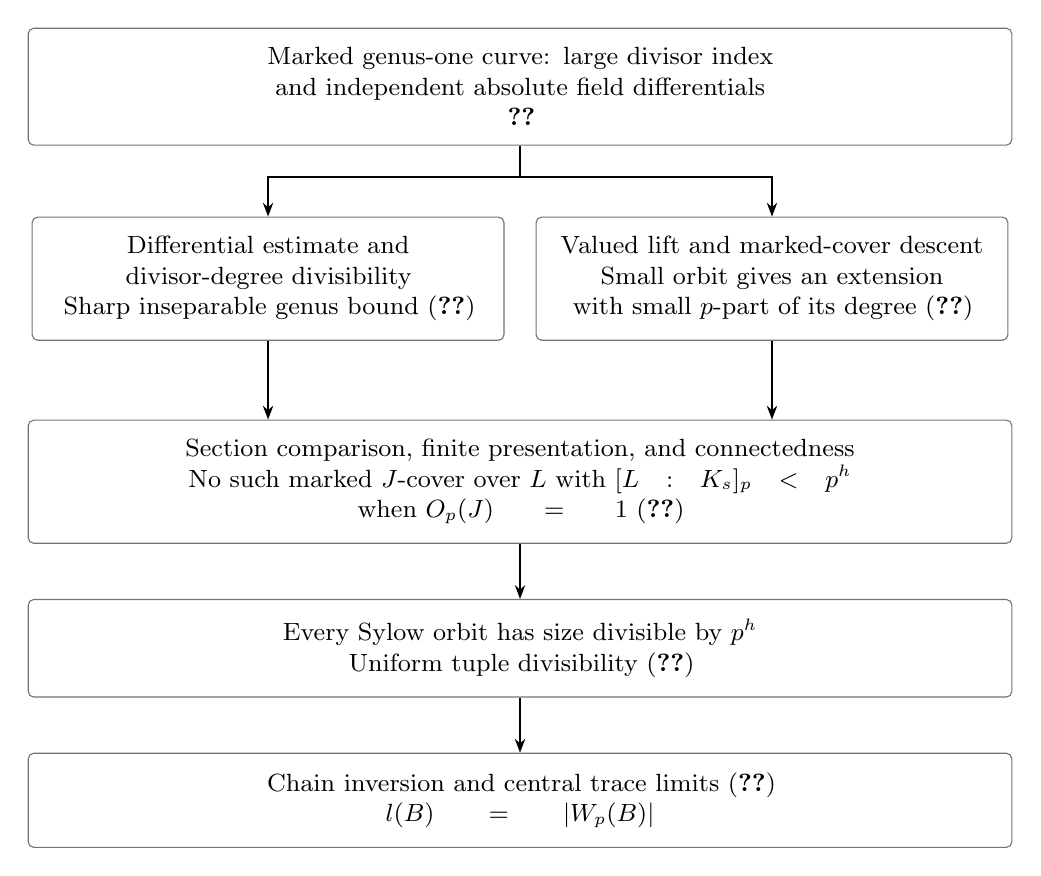
\begin{tikzpicture}[
  every node/.style={font=\small,align=center},
  stage/.style={draw=black!55,rounded corners=2pt,inner sep=7pt},
  flow/.style={-{Stealth[length=5pt]},semithick}
]
\node[stage,text width=12cm] (twist)
  {Marked genus-one curve: large divisor index\\
   and independent absolute field differentials\\
   \Cref{sec:twist}};
\coordinate (branch-top) at ($(twist.south)+(0,-9mm)$);
\coordinate (branch-split) at ($(twist.south)+(0,-4mm)$);
\node[stage,text width=5.5cm,anchor=north] (genus)
  at ($(branch-top)+(-3.2cm,0)$)
  {Differential estimate and divisor-degree divisibility\\Sharp inseparable genus bound
   (\Cref{sec:differentials})};
\node[stage,text width=5.5cm,anchor=north] (lift)
  at ($(branch-top)+(3.2cm,0)$)
  {Valued lift and marked-cover descent\\Small orbit gives an extension
   with small $p$-part of its degree
   (\Cref{sec:valuations})};
\node[fit=(genus)(lift),inner sep=0pt,outer sep=0pt] (branches) {};
\node[stage,text width=12cm,below=10mm of branches] (specialization)
  {Section comparison, finite presentation, and connectedness\\
   No such marked $J$-cover over $L$ with $[L:K_s]_p<p^h$\\
   when $O_p(J)=1$
   (\Cref{sec:specialization})};
\node[stage,text width=12cm,below=7mm of specialization] (count)
  {Every Sylow orbit has size divisible by $p^h$\\
   Uniform tuple divisibility (\Cref{thm:tuple-divisibility})};
\node[stage,text width=12cm,below=7mm of count] (blocks)
  {Chain inversion and central trace limits (\Cref{sec:group})\\
   $l(B)=|W_p(B)|$};
\draw[flow] (twist.south) -- (branch-split) -| (genus.north);
\draw[flow] (twist.south) -- (branch-split) -| (lift.north);
\draw[flow] (genus.south) -- (genus.south |- specialization.north);
\draw[flow] (lift.south) -- (lift.south |- specialization.north);
\draw[flow] (specialization.south) -- (count.north);
\draw[flow] (count.south) -- (blocks.north);
\end{tikzpicture}
\caption{Mathematical dependencies, not reading order. The covers are geometrically
connected $J$-Galois covers, with specified $J$-action over their field of
definition, branched only at the marked points and with inertia order
divisible by $p$ at every marked point. The two branches provide, respectively, the
genus estimate and the arithmetic realization of a hypothetical small
Sylow orbit. For sufficiently large $s$, their combination rules out such a cover over a field whose
degree has small $p$-part; the geometric cover degree is fixed at $|J|$.
The resulting uniform
divisibility supplies the counting hypothesis of the block-algebra
reduction, which is proved before the geometric construction and applied
at the end. No weight-counting theorem is used to construct the curves.}
\label{fig:proof-interfaces}
\end{figure}


\subsection*{Conventions}

All groups are finite. The identity is a $p$-element; a $p$-singular element has order divisible by $p$. We use $[x,y]=xyx^{-1}y^{-1}$ and write $O_p(X)$ for the largest normal $p$-subgroup of $X$. All curve degrees and coherent Euler characteristics are taken over the ground field specified at that point. A regular curve over an imperfect field is not presumed smooth or geometrically reduced. For such a projective curve $C$, we set
\[
 \chi(C)=\chi(\mathcal O_C),\qquad \nu(C)=-2\chi(C).
\]
These quantities add on disjoint unions. A valuation is written additively. A field extension is \emph{immediate} if it changes neither the value group nor the residue field.

\section{Classical foundations used}\label{sec:foundations}

We state the classical inputs to make the scope of the proof explicit. We also use elementary linear algebra, field and group theory, and the basic definitions and functorial formalism of schemes, sheaves, divisors, and K\"ahler differentials. The counting, index, inseparable-genus, valued-field, and specialization assertions particular to this proof are established in the later sections. In particular, no weight-counting theorem or conjectural reduction is an input.

\begin{foundation}[Finite groups]\label{foundation:groups}
For a finite group $X$, its $p$-subgroups lie in Sylow subgroups of order $|X|_p$. A nontrivial finite $p$-group has nontrivial center and an element of order $p$, and each of its maximal proper subgroups is normal. We use the orbit--stabilizer formula and the usual fixed-point and conjugation actions.
\end{foundation}

\begin{foundation}[Finite-dimensional algebras and characters]\label{foundation:algebra}
The Jacobson radical of a finite-dimensional algebra is nilpotent. Over an algebraically closed field, its semisimple quotient is a product of full matrix algebras, one for each simple module up to isomorphism. A finite-dimensional commutative algebra over an algebraically closed field is a product of local algebras with that field as residue, indexed by its primitive idempotents. Finite group algebras in characteristic zero are semisimple. Over a splitting field the simple endomorphism algebras are the scalar field, and an ordinary irreducible character satisfies
\[
 \sum_{x\in X}\chi(x)\chi(x^{-1})=|X|.
\]
Idempotents lift uniquely from the residue algebra of a finite commutative algebra over a complete discrete valuation ring. Nakayama's lemma applies to finite modules over any local ring.
\end{foundation}

\begin{foundation}[Commutative algebra]\label{foundation:commalg}
A finite-type algebra over a Noetherian ring is Noetherian. Integral extensions satisfy lying over. Closed points of a variety over a field are dense and have finite residue fields over the ground field. For an integral variety, the local dimension at a point plus the transcendence degree of its residue field is the transcendence degree of the function field. A regular local ring is a normal domain; a part of a minimal system of generators of its maximal ideal is a regular sequence and its quotient is regular of the correspondingly smaller dimension. A one-dimensional Noetherian normal local domain is a discrete valuation ring, as is a Noetherian local domain with nonzero principal maximal ideal. Finite torsion-free modules over discrete valuation rings are free. Completion of a discrete valuation ring retains its residue field and uniformizer.
\end{foundation}

\begin{foundation}[Fields and absolute field differentials]\label{foundation:fields}
If a finite group $D$ acts faithfully by automorphisms on a field $M$, then $M/M^D$ is Galois of degree $|D|$. Finite separable field extensions are simple. A finite field extension has a maximal separable subextension, and the remaining extension is purely inseparable; the number of embeddings in an algebraic closure is the separable degree. Multiplicative groups of finite fields are cyclic. Algebraically closed fields are classified by their characteristic and transcendence degree. If $S$ is a finitely generated field of transcendence degree $\rho$ over a perfect field $\kappa$, then
\[
 \dim_S\Omega_{S/\kappa}=\rho;
 \qquad [S:S^p]=p^\rho\quad\text{in characteristic }p.
\]
\end{foundation}

\begin{foundation}[Valuations over a complete discrete base]\label{foundation:valuation}
A valuation extends to an algebraic field extension. A complete discrete valuation on a field extends uniquely to any finite field extension; its valuation ring is the integral closure of the original ring, is finite over it, and is again a complete discrete valuation ring. The fields to which we apply the latter assertion initially have characteristic zero. No corresponding finiteness assertion for an arbitrary nondiscrete valuation ring is assumed.
See \cite[Tag 00IA]{Stacks} for prolongation and
\cite[Tags 032W, 09EM and 0325]{Stacks} for the complete
discrete-base finiteness assertions.
\end{foundation}

\begin{foundation}[Descent and finite models]\label{foundation:descent}
A projective scheme with a semilinear descent datum under a finite Galois field extension descends if equipped with a compatible linearized ample line bundle. The same statement holds for a finite \emph{\'etale} faithfully flat Galois extension of rings and a relatively ample line bundle. Equivariant morphisms and invariant closed subschemes descend along with the scheme. Flatness, smoothness, finiteness, \emph{\'etaleness}, and relative ampleness in these settings are checked after the faithfully flat extension. Geometric integrality of a finite-type scheme over a field can be checked after an extension of that field. A finite diagram of projective schemes and morphisms of finite presentation over a directed union of fields is defined over a finite stage, including its maps to a base scheme already defined there and the identities among those maps. One may realize projective descent by descent of semilinear modules and graded algebras followed by $\Proj$.
For the projective and module descent assertions, see \cite[Tags 0CCJ, 0CDR and 0D1V]{Stacks}.
The five locality assertions are respectively
\cite[Tags 02L2, 02VL, 02LA, 02VN and 0D3C]{Stacks}; geometric
integrality is covered by \cite[Tags 038K, 0384 and 054P]{Stacks}.
The finite-stage assertion follows from \cite[Tags 01ZM and 01ZP]{Stacks},
including chosen projective embeddings among the finite data.
\end{foundation}

\begin{foundation}[Normalization]\label{foundation:normalization}
The normalization of an integral variety over a field in a finite extension of its function field is finite. The normalization of a finite-type $\mathbb Z$-domain in its fraction field is finite. In the integral closure of a normal domain in a finite Galois extension of its fraction field, the Galois group acts transitively on the primes above any fixed prime of the base.
The normalization finiteness assertions follow from the Nagata property in \cite[Tag 0335]{Stacks}.
\end{foundation}

\begin{foundation}[Regularity, smoothness, and properness]\label{foundation:regularity}
Finite separable scalar extension preserves regularity and reducedness. Smooth varieties over a field are regular. A regular local ring essentially of finite type over a perfect field $\kappa$ is smooth at the corresponding point of a finite-type $\kappa$-model; its module of absolute differentials is free of rank the transcendence degree of the function field over $\kappa$. We use the valuative criterion for properness, including the unique extension of maps from fraction fields of valuation rings, and that proper maps are closed.
For regularity and smoothness over a perfect field, see \cite[Tags 00TV and 0B8X]{Stacks}.
\end{foundation}

\begin{foundation}[Proper cohomology and ample section rings]\label{foundation:cohomology}
Over a Noetherian base, the higher direct images of coherent sheaves under a proper morphism are coherent. Over an affine base their cohomology commutes with flat affine base change. For a projective scheme over an affine Noetherian base and a relatively ample line bundle, sufficiently high powers give projective embeddings, and sufficiently high twists annihilate higher coherent cohomology. The ample section ring is finitely generated and its $\Proj$ recovers the scheme. Finite pullback preserves ampleness; tensor products of relatively ample line bundles are relatively ample, and a line bundle is relatively ample if a positive power is. Formation of $\Proj$ commutes with base change. On a projective curve over a field, coherent cohomology vanishes in degrees greater than one, and for sheaves of finite support in degrees greater than zero. Global functions on a geometrically integral projective variety over a field equal the ground field.
For proper coherence, flat cohomology base change, and ample twists, respectively, see \cite[Tags 02O5, 02KH and 0B5T]{Stacks}.
For Proj recovery and the ampleness rules, see
\cite[Tags 0EKI, 0892, 0890 and 02NN]{Stacks}.
\end{foundation}

\begin{foundation}[Differentials, adjunction, and duality]\label{foundation:duality}
We use the transitivity sequence
\[
 \Omega_{V/U}\otimes_VW\longrightarrow\Omega_{W/U}
 \longrightarrow\Omega_{W/V}\longrightarrow0
\]
and the conormal sequence for a closed immersion. Let $S$ be a field. On $\mathbb P^b_S$,
$\det\Omega_{\mathbb P^b_S/S}=\mathcal O(-b-1)$. For a coherent sheaf $\mathcal G$ there, Serre duality identifies
\[
 H^i(\mathcal G)^\vee
 \simeq\operatorname{Ext}^{b-i}
       (\mathcal G,\mathcal O(-b-1)).
\]
We use the local-to-global Ext spectral sequence and the Koszul resolution of a quotient by a regular sequence. These inputs will yield the required absolute determinant-degree formula even when the curve is not smooth over $S$.
For the projective-space dualizing complex and the adjunction formalism, see \cite[Tag 0A9W and Section~48.15]{Stacks}.
The local-to-global Ext sequence is \cite[Tag 0BQP]{Stacks}.
\end{foundation}

\begin{foundation}[Elliptic curves]\label{foundation:elliptic}
A smooth Weierstrass cubic with its point at infinity is an elliptic curve. A generalized Weierstrass equation over a discrete valuation ring with unit discriminant gives a smooth elliptic scheme, polarized by three times its origin. Its relative cotangent line is trivial with invariant differential $\eta$, and multiplication by an integer $a$ pulls $\eta$ back to $a\eta$. For a positive integer $a$, multiplication by $a$ on an elliptic curve or elliptic scheme is finite locally free of degree $a^2$.
For the relative group law, see
\cite[II, Proposition~2.7]{DeligneRapoport1973}; the unit-discriminant
Weierstrass family and the invariant cotangent description are given in
\cite[Tags 072S and 047I]{Stacks}. See also
\cite[Chapter~III]{Silverman2009} for the Weierstrass formulation.
Multiplication is finite flat and surjective by
\cite[Proposition~20.7]{MilneAV2022}; over the Noetherian bases here it
is finite locally free by \cite[Tag 02KB]{Stacks}.
\end{foundation}

\begin{foundation}[Complex curves and covers]\label{foundation:complex}
Finite \'etale algebraic covers of a smooth complex algebraic curve
correspond to finite unramified topological covers of its analytification,
including morphisms. For a punctured projective curve, normalization of
the original projective curve in the resulting algebraic function field
gives the finite compact cover. Normal complex curves are smooth, and the
local punctured covering completes by a power map, so monodromy cycle
lengths give ramification indices. Topological covers are classified by
fundamental-group actions on finite fibers. The fundamental group of a
genus-one surface punctured at $n$ points has generators
$x,y,u_1,\ldots,u_n$ with the single relation
\[
 [x,y]u_1\cdots u_n=1.
\]
For a finite map of smooth proper curves over an algebraically closed field of characteristic zero, Riemann--Hurwitz states
\[
 2g(C)-2=\deg(f)\bigl(2g(C')-2\bigr)
              +\sum_{P\in C}(e_P-1).
\]
For the algebraic/topological cover correspondence, see \cite[Theorem~3.4]{MilneLEC2008}; for Riemann--Hurwitz, see \cite[Section~53.12, Tag 0C1B]{Stacks}.
\end{foundation}

\begin{foundation}[Noetherian connectedness]\label{foundation:connectedness}
A proper morphism over a locally Noetherian base whose structure-sheaf direct image is canonically the structure sheaf of the base has geometrically connected fibers. This is the connected-fiber assertion of Stein factorization. We apply it only after constructing a Noetherian normal model, not directly over the nondiscrete valuation ring.
See \cite[Tag 03H0]{Stacks}.
\end{foundation}

\subsection{Coefficient fields and scalar extension}\label{sec:coefficients}

We justify the coefficient choice in \Cref{sec:introduction} without
requiring a mixed-characteristic lift of every algebraically closed
field. Put $\kappa=\overline{\mathbb F}_p$ and choose an embedding
$\kappa\hookrightarrow k$. For any finite group $X$, the ideal
$\rad(\kappa X)\otimes_\kappa k$ is nilpotent, and the quotient of
$kX$ by this ideal is the scalar extension of the split matrix product
$\kappa X/\rad(\kappa X)$. That quotient is again a split semisimple
algebra. The ideal is therefore exactly $\rad(kX)$, and the simple
modules correspond under scalar extension.

The center also commutes with this extension: it is the kernel of the
finitely many linear maps $a\mapsto ax-xa$, $x\in X$, and field
extension preserves kernels. Each local factor of $Z(\kappa X)$ has
nilpotent radical and residue $\kappa$; after extension it still has
nilpotent radical, now with residue $k$, so remains local. Thus
primitive blocks correspond and their simple-module counts agree.
Coefficient restriction, restriction to centralizers in the Brauer
map, and the quotient maps for normal subgroups all commute with
scalar extension. The residue characters of the local central factors
extend as well. Consequently the central-character block assignment
in \eqref{eq:block-assignment} is preserved, for every subgroup and
subquotient involved in a weight. It suffices to prove the numerical
identity over $\kappa$.

To construct the coefficient ring, start with $\mathbb Z_p$, lift a
tower of finite separable extensions of its residue field $\mathbb F_p$
that exhausts $\kappa$, and complete the union. The construction at the
start of the proof of \Cref{prop:mixed-lift} shows that this gives a
complete discrete valuation ring of characteristic zero with residue
$\kappa$.
In an algebraic closure of its fraction field, choose matrix
realizations of every ordinary irreducible representation of every
subgroup of $G$. There are only finitely many such representations and
matrix entries. Adjoining their entries gives a finite field extension
that splits all those subgroups. Its valuation ring is again a complete
DVR by \Cref{foundation:valuation}; its finite residue extension is
still $\kappa$, which is algebraically closed. This gives the system
$(K,\mathcal O,\kappa)$ used in \Cref{sec:group}. Quotient
representations inflate, so the same coefficients split the required
subquotients. These coefficient fields are separate from the auxiliary
geometric fields constructed later.

The remaining sections prove the blockwise chain identity, the marked
high-index twist, the genus estimate with exact rounding, the required
valued-field assertions, and the specialization model. The foundations
above supply their classical inputs, not the desired weight equality.

\section{From block counts to generating tuples}\label{sec:group}

Fix a prime $p$. Write $O_p(X)$ for the largest normal $p$-subgroup
of a finite group $X$, and put $[x,y]=xyx^{-1}y^{-1}$. A
$p$-element includes the identity; a $p'$-element has order prime to
$p$; and a $p$-singular element has order divisible by $p$.
The geometric sections will establish the following precise counting
statement. Its uniformity is part of the assertion.

\begin{theorem}[Uniform divisibility for generating tuples]
\label{thm:tuple-divisibility}
Let $J$ be a finite group with $O_p(J)=1$. For $s\geq0$, $n=p^s$,
and a multiset
$\mathcal M$ of $n$ conjugacy classes of $p$-singular elements of $J$,
let $N_{J,s}(\mathcal M)$ be the number, modulo simultaneous
$J$-conjugation, of ordered tuples
\[
 (x,y,u_1,\ldots,u_n)\in J^{n+2}
\]
satisfying
\begin{equation}\label{eq:tuple-relation}
 [x,y]u_1\cdots u_n=1,\qquad
 \langle x,y,u_1,\ldots,u_n\rangle=J,
 \qquad \{[u_1],\ldots,[u_n]\}=\mathcal M.
\end{equation}
For every integer $h\geq1$, there is an integer $s_0=s_0(p,J,h)$
such that
\[
 p^h\mid N_{J,s}(\mathcal M)
 \qquad(s\geq s_0)
\]
for every such multiset $\mathcal M$.
\end{theorem}

The entries $u_i$ remain ordered: prescribing their multiset of classes
does not quotient by permutations. Empty tuple sets have count zero,
so the statement includes $J=1$ and groups of order prime to $p$.
The proof of \Cref{thm:tuple-divisibility} is completed after
\Cref{prop:no-small-cover}. This section proves that it implies the
block equality, using \Cref{foundation:groups,foundation:algebra}
and proving the required counting reductions explicitly.

\subsection{Coefficient projection and the weight transform}

For each ambient finite group $X$, choose a splitting coefficient system
$(K,\mathcal O,k)$ as in \Cref{sec:introduction,sec:coefficients}, with
$X$ in place of $G$. Hold this system fixed throughout the calculations
with $X$ and its subquotients.
This system also splits all subquotients that occur below: a subgroup of a
quotient lifts to a subgroup by taking its preimage, and a
representation of a quotient inflates to that preimage. These
observations apply after any number of subgroup and quotient steps.
Ordinary irreducibles may therefore be realized over $K$. Their
identification with complex irreducibles, when needed, follows by
first splitting the group algebra over $\overline{\mathbb Q}$ and
then extending scalars to algebraically closed characteristic-zero
fields.

For a central idempotent $E\in kX$, define
\begin{align*}
 l(X,E)&=\#\{\text{simple $kX$-modules selected by $E$}\},\\
 k_{\mathrm{ord}}(X,E)&=\#\{\text{ordinary irreducibles selected by the lift of $E$}\},\\
 z(X,E)&=\#\{\chi\text{ selected by that lift}:\chi(1)_p=|X|_p\}.
\end{align*}
Here and throughout, modules and characters are counted up to
isomorphism. The class sums form a basis of $Z(\mathcal O X)$, and
their reductions form a basis of $Z(kX)$. Idempotent lifting over the
complete DVR thus gives a unique central idempotent lifting $E$.
Every integral central element acts on an ordinary irreducible by
a scalar in $\mathcal O$: the scalar lies in $K$ by splitting and
satisfies a monic integral equation by finiteness, and $\mathcal O$
is integrally closed. Reduction of this scalar defines a character
of $Z(kX)$. The Artinian local decomposition of that center shows
that it is precisely $\lambda_b$, where $b$ is the block containing
the ordinary irreducible.

For $H\leq X$, let $s_H$ denote coefficient restriction from
$Z(kX)$ to $Z(kH)$, or its integral analogue when appropriate.
For a $p$-subgroup $Q$, let $\operatorname{Br}_Q$ denote restriction
of coefficients from the $Q$-invariants $(kX)^Q$ to $kC_X(Q)$.

\begin{lemma}[Normalizer projection]\label{lem:normalizer-projection}
The map $\operatorname{Br}_Q:(kX)^Q\longrightarrow kC_X(Q)$ is a
unital algebra homomorphism. Suppose that
\[
 Q\leq H\leq N_X(Q),\qquad C_X(Q)\leq H.
\]
Writing $\pi_Q:kH\longrightarrow k[H/Q]$ for the quotient map, one
has, for $v\in Z(kX)$,
\begin{equation}\label{eq:normalizer-projection}
 \pi_Q(s_H(v))=\pi_Q(\operatorname{Br}_Q(v)),
 \qquad
 \lambda_b(s_H(v))=\lambda_b(\operatorname{Br}_Q(v))
\end{equation}
for every block $b$ of $H$. In particular $\lambda_b\circ s_H$ is
the central character of a unique block of $X$.
\end{lemma}

\begin{proof}
To compute the coefficient of $g\in C_X(Q)$ in a product of two
$Q$-invariant elements, let $Q$ conjugate the pairs $(a,b)$ with
$ab=g$. Coefficient products are constant on the orbits. Every
nontrivial orbit has size divisible by $p$, and the fixed pairs are
exactly those with $a,b\in C_X(Q)$. This proves multiplicativity;
the identity is preserved.

Each coset $hQ$ is stable under conjugation by $Q$, because
$h\in N_X(Q)$. Applying the same orbit cancellation to the sum
of coefficients over that coset proves the first identity in
\eqref{eq:normalizer-projection}. Also
$\operatorname{Br}_Q(v)\in Z(kH)$, since its support lies in
$C_X(Q)\leq H$ and it is invariant under $H$.

Every nonzero module for a finite $p$-group over $k$ has nonzero
invariants. For completeness, choose a central element $z$ of order
$p$; the nonzero kernel of $z-1$, whose $p$th power is zero, is a
module for the smaller group $Q/\langle z\rangle$, and induction
applies. If the module is simple for $H$, its $Q$-invariants are
$H$-stable, and hence the whole module. Thus every simple $kH$-module
factors through $H/Q$, proving the second identity. The composition
with $\operatorname{Br}_Q$ is a unital algebra character. Characters
of the finite commutative algebra $Z(kX)$ are its local residue
characters, one for each block, giving uniqueness.
\end{proof}

For $H=N_X(Q)$ put
\[
 \overline E_Q
   =\pi_Q(s_H(E))
   =\pi_Q(\operatorname{Br}_Q(E))\in Z(k[H/Q]).
\]
This is an idempotent. Its selected defect-zero quotient characters
are exactly the weights assigned to the blocks appearing in $E$.
Indeed, the lift of $\operatorname{Br}_Q(E)$ maps to the lift of
$\overline E_Q$ by uniqueness of central idempotent lifting. Its
action on the inflation of a quotient character is therefore one
exactly when the latter is selected by $\overline E_Q$. If $b$ is
the block of this inflation, the same test is
\[
 \lambda_b(\operatorname{Br}_Q(E))
   =\lambda_b(s_H(E))=1.
\]
By \Cref{lem:normalizer-projection}, this says that the induced block
is one of the blocks in $E$, with the coefficient-projection
definition in \eqref{eq:block-assignment}. Once $Q$ is fixed up to $X$-conjugacy,
there is no further identification of its quotient characters:
$N_X(Q)$ acts on $N_X(Q)/Q$ by inner automorphisms.

For a conjugation-invariant function $g$ of such pairs $(X,E)$,
define
\begin{equation}\label{eq:weight-transform}
 (Tg)(X,E)=
 \sum_{\substack{1<Q\leq X\text{ a $p$-subgroup}\\
                  \text{up to }X\text{-conjugacy}}}
 g\bigl(N_X(Q)/Q,\overline E_Q\bigr).
\end{equation}
Consequently the desired universal equality for block sums is
$l=(1+T)z$. The identity term includes precisely $Q=1$.
Every transition in $T$ strictly decreases the $p$-part of the group
order, so $T$ is nilpotent on each evaluated pair. Thus the formal
inverse $(1+T)^{-1}=\sum_{r\geq0}(-T)^r$ is evaluation-wise finite.

The next step makes the connection with subgroup-chain formulations of
the weight conjecture \cite{KnorrRobinson1989}. We derive the particular
normal-chain identity from this finite inverse, retaining its idempotent
and orbit data throughout.

\begin{definition}[Chains]\label{def:p-chains}
A chain in $X$ is a strictly increasing sequence of $p$-subgroups
\[
 \mathcal C=(1=Q_0<Q_1<\cdots<Q_r),
 \qquad |\mathcal C|=r.
\]
The length-zero chain $(1)$ is included. Set
\[
 H_{\mathcal C}=\bigcap_{i=0}^rN_X(Q_i),
 \qquad E_{\mathcal C}=\operatorname{Br}_{Q_r}(E).
\]
Call $\mathcal C$ \emph{normal} if every $Q_i$ is normal in $Q_r$.
\end{definition}

For every chain, normal or otherwise,
$C_X(Q_r)\leq H_{\mathcal C}\leq N_X(Q_r)$, so
$E_{\mathcal C}$ is an idempotent of $Z(kH_{\mathcal C})$.
For a normal chain one also has $Q_r\leq H_{\mathcal C}$.

\begin{lemma}[Finite chain inversion]\label{lem:chain-transform}
The identity $l=(1+T)z$ for all pairs $(X,E)$ is equivalent to
\begin{equation}\label{eq:chain-inversion}
 z(X,E)=
 \sum_{\substack{\mathcal C/X\\\mathcal C\ \mathrm{normal}}}
 (-1)^{|\mathcal C|}l(H_{\mathcal C},E_{\mathcal C}),
\end{equation}
where $\mathcal C/X$ denotes one representative of each
$X$-conjugacy orbit.
\end{lemma}

\begin{proof}
We identify the terms of $T^r l$. After $r$ steps they correspond
to normal chains of length $r$, with group
$H_{\mathcal C}/Q_r$ and idempotent
\[
 \pi_{Q_r}(s_{H_{\mathcal C}}(E))
   =\pi_{Q_r}(E_{\mathcal C}).
\]
For the induction, the preimage $Q_{r+1}$ of a nontrivial
$p$-subgroup of $H_{\mathcal C}/Q_r$ is a $p$-group strictly
containing $Q_r$. It lies in $H_{\mathcal C}$ and therefore
normalizes every preceding $Q_i$. Conversely every normal one-step
extension arises in this way. Its normalizer in the quotient has
preimage
$H_{\mathcal C}\cap N_X(Q_{r+1})=H_{\mathcal C'}$.
After fixing $\mathcal C$, conjugation is by its stabilizer
$H_{\mathcal C}$, which is exactly quotient conjugation at the next
step. This proves the orbit assertion without an extra multiplicity.

To check the idempotent at the next step, write
$E=\sum_{x\in X}e_xx$ and put $H'=H_{\mathcal C'}$.
The new normalizer in $H_{\mathcal C}/Q_r$ is $H'/Q_r$.
Restriction to this normalizer retains exactly the coefficient sums
over the $Q_r$-cosets contained in $H'$. Choose a set $A$ of
representatives for the cosets of $Q_r$ in $Q_{r+1}$. For $h\in H'$,
the subsequent quotient has coefficient
\[
 \sum_{a\in A}\ \sum_{q\in Q_r}e_{haq}
     =\sum_{t\in Q_{r+1}}e_{ht}
\]
at $hQ_{r+1}$: the sets $aQ_r$, $a\in A$, partition $Q_{r+1}$.
These are precisely the coefficients of
$\pi_{Q_{r+1}}(s_{H'}(E))$.
By \Cref{lem:normalizer-projection}, this idempotent is
$\pi_{Q_{r+1}}(E_{\mathcal C'})$, as required.
Every simple $kH_{\mathcal C}$-module factors through
$H_{\mathcal C}/Q_r$ and has the indicated idempotent action.
Hence the contribution to $T^rl$ is the corresponding term in
\eqref{eq:chain-inversion}. The finite inverse of $1+T$ now gives
the equivalence.
\end{proof}

\subsection{Cocenters and subsections}

By \Cref{lem:chain-transform}, the remaining algebraic objective is
\eqref{eq:chain-inversion}. We next express ordinary character counts
as sums of simple-module counts in centralizers. Chain cancellation
will then replace the alternating sum of $l$ by an alternating sum of
$k_{\mathrm{ord}}$, which can be computed by central traces.

For an algebra $A$, write $V(A)=A/[A,A]$, where $[A,A]$ is the
linear span of commutators, and write $\overline a$ for the image of
$a$. A central element acts on $V(A)$ by multiplication.

Powers modulo commutators underlie K\"ulshammer's generalized Reynolds
ideals; see \cite[Section~2]{HHKM2005}. We give the finite-dimensional
argument needed to extract the two block counts.

\begin{lemma}[Cocenter ranks]\label{lem:cocenter-ranks}
For a finite-dimensional $k$-algebra $A$, the map
\[
 F_A:V(A)\longrightarrow V(A),\qquad
 \overline a\longmapsto\overline{a^p}
\]
is well-defined and Frobenius semilinear. Its stable image has
dimension equal to the number of simple $A$-modules, and its
summand selected by a central idempotent has dimension equal to
the corresponding simple-module count.
For $A=kX$, this stable image is the span of the $p'$-classes.
The ranks of multiplication by $E$ on that span and on all of
$V(kX)$ are, respectively, $l(X,E)$ and $k_{\mathrm{ord}}(X,E)$.
\end{lemma}

\begin{proof}
In the expansion of $(a+b)^p$, cyclic rotations of any mixed word
give the same cocenter class. Their orbits have size $p$, leaving
only $a^p$ and $b^p$. Thus the power operation into the cocenter
is additive and is Frobenius semilinear. Moreover
$\overline{(ab)^p}=\overline{(ba)^p}$, by one cyclic rotation;
additivity shows that this operation kills the linear commutator
space. It therefore descends to $F_A$.

Let $R$ be the Jacobson radical of $A$. The kernel of
$V(A)\longrightarrow V(A/R)$ is represented by elements of $R$:
lift any commutator expression downstairs and subtract it upstairs.
Since $R$ is nilpotent, a sufficiently high iterate of $F_A$ kills
this kernel. On the split semisimple algebra $A/R$, the cocenter
has one matrix-trace coordinate per simple factor, and $F_A$
raises each coordinate to the $p$th power. It is bijective because
$k$ is perfect. For example, the trace identity here follows by
triangularizing a matrix over $k$ and taking the $p$th powers of
its diagonal entries.

The descending images of $F_A$ stabilize, since they are
$k$-subspaces of a finite-dimensional space. Denote the stable image
by $S$ and the quotient map by $q:V(A)\to V(A/R)$.
Choose $m$ large enough that $S=\operatorname{im}F_A^m$ and
$F_A^m$ kills $\ker q$. On $S$, the map $F_A$ is surjective
and hence bijective, because it is semilinear for the automorphism
$a\mapsto a^p$ of the perfect field $k$. If $x\in S\cap\ker q$,
then $F_A^m(x)=0$; injectivity on $S$ gives $x=0$.
To prove surjectivity of $q|_S$, take $y\in V(A/R)$. The
Frobenius map $F_{A/R}$ is bijective, so choose $y'$ with
$F_{A/R}^m(y')=y$ and lift $y'$ to $x\in V(A)$. Then
$F_A^m(x)\in S$ and $q(F_A^m(x))=y$. Thus $q|_S$ is an
isomorphism. Finally
$(Ea)^p=Ea^p$ for a central idempotent $E$, so all these statements
respect its summand.

For a group algebra the cocenter is free on conjugacy classes,
represented by individual group elements: the commutator
relations identify exactly conjugate elements. Sufficiently high
$p$-powers land on $p'$-elements, and taking $p$th powers permutes
the $p'$-classes. This identifies the stable image. The integral
cocenter $V(\mathcal O X)$ is free on the same class basis. The
lift of $E$ projects it onto a free direct summand, whose rank is
unchanged over $k$ and $K$. Split semisimplicity over $K$ identifies
this rank with $k_{\mathrm{ord}}(X,E)$.
\end{proof}

Every group element has a unique commuting factorization into its
$p$-part and $p'$-part, both powers of that element. A
\emph{section} is the set of elements whose $p$-parts are conjugate
to a fixed $p$-element.

The next identity is Brauer's classical subsection count
\cite{Brauer1959}. The cocenter argument also proves the support
property needed for the defect-zero detector, without dividing by
class sizes in characteristic $p$.

\begin{lemma}[Subsection formula and support]\label{lem:subsections}
For every central idempotent $E\in kX$,
\begin{equation}\label{eq:subsections}
 k_{\mathrm{ord}}(X,E)=
 \sum_{\substack{[u]\text{ an }X\text{-class}\\u\text{ a }p\text{-element}}}
 l\bigl(C_X(u),\operatorname{Br}_{\langle u\rangle}(E)\bigr).
\end{equation}
Multiplication by $E$ preserves the section decomposition of the
cocenter and the section decomposition of the center into spans
of class sums.
\end{lemma}

\begin{proof}
Fix a $p$-element $u$ and set $C=C_X(u)$. The map
$\overline t\mapsto\overline{ut}$ identifies the $p'$-class span
of $V(kC)$ with the section span belonging to $u$ in $V(kX)$.
It is a bijection of class bases: conjugacy of $ut$ and $ut'$
forces a conjugating element to centralize their common $p$-part
$u$, and the converse is immediate.

For $t\in C$ a $p'$-element, conjugation by $\langle u\rangle$
in the expansion of $Eut$ gives
\[
 \overline{Eut}
   =\overline{\operatorname{Br}_{\langle u\rangle}(E)ut}.
\]
Indeed, the coefficients are constant on these orbits and the
cocenter classes of their products with $ut$ agree; only fixed
orbits survive. The restricted idempotent is central in $kC$ and
preserves its $p'$-class span by \Cref{lem:cocenter-ranks}.
Multiplication by $u$ is central in $kC$, so the displayed
identification intertwines the two idempotent actions. Their ranks
are thus the terms in \eqref{eq:subsections}. Summing the ranks
over the sections proves that identity.

For the center, use the pairing
\[
 Z(kX)\times V(kX)\longrightarrow k,
 \qquad (a,\overline b)\longmapsto\tau(ab),
\]
where $\tau$ takes the coefficient of $1$. It is nondegenerate:
a class sum pairs with an individual representative of its inverse
class with coefficient one. Multiplication by $E$ is self-adjoint
for this pairing. Sections on the center pair with the inverse
sections of the cocenter, so preservation there proves preservation
here. In particular no class-size division is involved.
\end{proof}

\subsection{Two cancellations on chain orbits}

\begin{lemma}[Removal of nonnormal chains]\label{lem:nonnormal-cancellation}
In an alternating sum over chain orbits, every contribution that
depends only on $H_{\mathcal C}$ and $Q_r$ cancels on the nonnormal
chains. Thus such a sum may be taken over all chains or only normal
chains.
\end{lemma}

\begin{proof}
For a nonnormal chain, let $i$ be the largest index for which
$A=Q_i$ is not normal in $P=Q_r$, and let $R$ be the normal closure
of $A$ in $P$. Then $A<R\leq Q_{i+1}$: every later member is
normal in $P$. Also $R<P$. To see the latter, put the proper
subgroup $A$ in a maximal subgroup of $P$, which is normal because
$P$ is a finite $p$-group; it contains $R$.

Insert $R$ immediately after $A$ if it is absent, and remove it
if it is present. The last group $P$ and the last nonnormal member
$A$ are unchanged, so this operation is an involution. Every
element normalizing $A$ and $P$ normalizes their normal closure
$R$; hence insertion or removal leaves $H_{\mathcal C}$ unchanged.
The operation commutes with $X$-conjugation and changes the length
by one. It induces a fixed-point-free sign reversal on the orbits,
which proves cancellation.
\end{proof}

\begin{lemma}[Alternating subsection cancellation]
\label{lem:alternating-subsections}
One has
\begin{equation}\label{eq:alternating-subsections}
 \sum_{\substack{\mathcal C/X\\\mathcal C\ \mathrm{normal}}}
 (-1)^{|\mathcal C|}l(H_{\mathcal C},E_{\mathcal C})
 =
 \sum_{\substack{\mathcal C/X\\\mathcal C\ \mathrm{normal}}}
 (-1)^{|\mathcal C|}k_{\mathrm{ord}}(H_{\mathcal C},E_{\mathcal C}).
\end{equation}
\end{lemma}

\begin{proof}
By \Cref{lem:nonnormal-cancellation}, both sums may be taken over
all chains. Expand the ordinary count by \Cref{lem:subsections}.
The $u=1$ terms give the simple-module sum. The other terms are
indexed by $X$-orbits of pairs $(\mathcal C,u)$, with $u\ne1$ a
$p$-element in $H_{\mathcal C}$. This orbit description follows
because the stabilizer of a fixed chain is $H_{\mathcal C}$.
The contribution of such a pair is
\begin{equation}\label{eq:pair-contribution}
 l\bigl(H_{\mathcal C}\cap C_X(u),
         \operatorname{Br}_{Q_r\langle u\rangle}(E)\bigr).
\end{equation}
Here $u$ normalizes $Q_r$, so $Q_r\langle u\rangle$ is a
$p$-group; successive coefficient restrictions have support
$C_X(Q_r)\cap C_X(u)=C_X(Q_r\langle u\rangle)$, proving the
idempotent in this expression.

Let $i$ be the largest index, allowing $0$ and $r$, for which
$u\notin Q_i$. Such an index exists since $Q_0=1$. Toggle
$R=Q_i\langle u\rangle$ immediately after $Q_i$: insert it
if absent, and remove it if present. It is a $p$-group, since
$u$ normalizes $Q_i$, and it is contained in every later member,
all of which contain $u$. The last member not containing $u$
therefore remains $Q_i$; this proves involutivity, including an
insertion after the terminal member and its inverse deletion.

Every element centralizing $u$ and normalizing $Q_i$ normalizes
$R$. Thus $H_{\mathcal C}\cap C_X(u)$ is unchanged. The product
of the terminal member with $\langle u\rangle$ is also unchanged,
even when the terminal member is inserted or deleted. Hence
\eqref{eq:pair-contribution} is preserved. The operation is
$X$-equivariant and reverses the sign, so all $u\ne1$ terms cancel.
\end{proof}

\subsection{Detecting defect zero by central elements}

By \Cref{lem:alternating-subsections}, it remains to prove that the
alternating ordinary-character sum in
\eqref{eq:alternating-subsections} equals $z(X,E)$. Their difference
retains the signed contributions of all characters selected by
$E_{\mathcal C}$ on positive-length normal chains, but omits the
selected defect-zero characters at the chain $(1)$. We will realize
this difference as a trace limit by constructing a central element
with the corresponding zero-or-one central-character values.

Put
\[
 c_X=\sum_{u\in X\,\text{a }p\text{-element}}u,
 \qquad d_X=\sum_{x,y\in X}[x,y],
 \qquad I_X(a)=\sum_{x\in X}xax^{-1}.
\]
These elements and the image of $I_X$ are central. Call a block
\emph{semisimple} if its algebra is semisimple; since a block has no
nontrivial central idempotent, such a block is one full matrix
algebra over $k$.

The scalar of $d_X$ will identify these semisimple blocks with the
ordinary defect-zero characters. The complement $1-c_X$ will then remove
exactly those blocks from the central trace, using the support
information supplied by $I_X$.

The operator $I_X$ is the group-algebra Higman trace
\cite[Section~2]{Higman1955}; see also
\cite[Sections~2.4--2.5]{LorenzTokoly2011}. The use of $c_X$ to
isolate defect zero goes back to Tsushima \cite[Theorem~1]{Tsushima1971}.
The following proof records the exact radical-annihilation and
central-character consequences used in our trace limit.

\begin{lemma}[Averaging and defect zero]\label{lem:defect-zero-detection}
The image of $I_X$, and also $d_X$, annihilates the Jacobson radical
of $kX$. On a semisimple block, $d_X$ has nonzero central scalar;
on every other block its central character is zero. Each semisimple
block contains exactly one ordinary irreducible, which has defect
zero, and every ordinary defect-zero irreducible occurs in this
way. Moreover:
\begin{enumerate}[label=\textup{(\roman*)}]
 \item $\operatorname{im}I_X$ is the span of class sums of elements
 whose centralizers have order prime to $p$;
 \item each semisimple block idempotent belongs to
 $\operatorname{im}I_X$ and has zero Brauer image at every nontrivial
 $p$-subgroup;
 \item $\lambda_b(c_X)=0$ on every nonsemisimple block $b$.
\end{enumerate}
\end{lemma}

\begin{proof}
\textit{Radical annihilation.}
The form $(a,b)\mapsto\tau(ab)$ on $kX$ is symmetric and
nondegenerate. For dual bases $v_i,v_i^*$, the tensor
$\Omega=\sum_i v_i\otimes v_i^*$ is independent of the chosen
bases. Apply the linear map $u\otimes v\mapsto uav$ to this
tensor. In the group basis, whose dual basis consists of the inverses,
the result is $I_X(a)$. Similarly, apply
$u\otimes v\otimes w\otimes z\mapsto uwvz$ to
$\Omega\otimes\Omega$. In the group basis the result is
$\sum_{x,y\in X}xyx^{-1}y^{-1}=d_X$. Thus in any dual bases
\begin{equation}\label{eq:averaging-tensor}
 I_X(a)=\sum_i v_iav_i^*,\qquad
 d_X=\sum_{i,j}v_iv_jv_i^*v_j^*
     =\sum_j I_X(v_j)v_j^*.
\end{equation}
For $b$ in the radical $R$, the trace identity
\[
 \tau(I_X(a)b)=\operatorname{Tr}(L_bR_a)
\]
follows by writing the trace in these dual bases; $L$ and $R$
denote left and right multiplication. Since $L_b$ is nilpotent
and commutes with $R_a$, this trace is zero. Replace $b$ by $bc$
for arbitrary $c\in kX$, and use nondegeneracy to obtain
$I_X(a)b=0$. The final expression in
\eqref{eq:averaging-tensor} then shows that $d_XR=0$ as well,
because $v_j^*R\subseteq R$.

\textit{Semisimple blocks and ordinary defect zero.}
Distinct block ideals are orthogonal for the form. On a
semisimple block $M_d(k)$ its restriction is $t\operatorname{Tr}$
for some $t\in k^\times$. Indeed a symmetric functional kills
commutators, whose quotient in a matrix algebra is the trace line,
and nondegeneracy forces $t\ne0$. Matrix units $e_{ij}$ have duals
$t^{-1}e_{ji}$. Since
$\sum_{i,j}e_{ij}ae_{ji}=\operatorname{Tr}(a)1$, the first
contraction in \eqref{eq:averaging-tensor} gives
$I_X(a)=t^{-1}\operatorname{Tr}(a)1$. In particular
$I_X(e_{ij})=t^{-1}\delta_{ij}1$, so its last expression gives
\[
 d_X=\sum_{i,j}I_X(e_{ij})t^{-1}e_{ji}
     =t^{-2}\sum_i e_{ii}=t^{-2}1.
\]
We have therefore proved
\begin{equation}\label{eq:simple-block-scalars}
 I_X(a)=t^{-1}\operatorname{Tr}(a)1,
 \qquad d_X=t^{-2}1
 \quad\text{on this block}.
\end{equation}
In particular its idempotent lies in the image of $I_X$; one can
take $a=te_{11}$. These formulas do not require $d$ to be nonzero
in $k$. On a nonsemisimple block, a central element with nonzero
residue scalar is a unit in its local center. Such a unit cannot
annihilate the nonzero radical. This proves the assertion about
the central character of $d_X$.

Now compute the same commutator sum in characteristic zero. If
$\chi$ has degree $d$, Schur's lemma gives
\[
 \sum_{x\in X}\rho(xyx^{-1})
      =\frac{|X|\chi(y)}d\,1.
\]
Multiply by $\rho(y^{-1})$, sum over $y$, and take traces.
Ordinary character orthogonality gives the scalar
\begin{equation}\label{eq:ordinary-commutator-scalar}
 \lambda_\chi(d_X)=\frac{|X|^2}{\chi(1)^2}.
\end{equation}
It is integral, by the integrality of ordinary central scalars.
Its reduction is nonzero exactly when
$v_p(\chi(1))=v_p(|X|)$, namely in defect zero. The modular
calculation therefore puts exactly these characters in
semisimple blocks. Such a block has cocenter dimension one, so
\Cref{lem:cocenter-ranks} shows that its lifted block selects
exactly one ordinary irreducible. This also proves existence of
that character.

\textit{Support and the $p$-element sum.}
For a group element $g$ one has
\[
 I_X(g)=|C_X(g)|\sum_{a\in[g]}a.
\]
This proves assertion (i). The support of a semisimple block
idempotent, already in this image, therefore contains no element
centralized by a nontrivial $p$-subgroup, proving (ii).

Finally fix a nontrivial $p$-subgroup $P$. Choose
$z\in Z(P)$ of order $p$. It is central also in $C_X(P)$, and
multiplication by $z$ preserves the set of $p$-elements of that
centralizer. With $q=\sum_{j=0}^{p-1}z^j$, the sum of those
$p$-elements factors as $q$ times a sum of orbit representatives.
As $q$ is central and $q^2=pq=0$, this proves
\[
 \operatorname{Br}_P(c_X)^2=0,
 \qquad \operatorname{Br}_P(c_X^2)=0.
\]
If $p$ divides $|C_X(g)|$, a nontrivial $p$-subgroup
$P\leq C_X(g)$ makes the coefficient of $g$ in $c_X^2$ vanish
by this identity. Assertion (i) gives $c_X^2\in\operatorname{im}I_X$.
On a nonsemisimple block its central character must therefore
vanish, by the same radical-annihilator argument. Since
$\lambda_b(c_X)^2=\lambda_b(c_X^2)=0$, assertion (iii) follows.
\end{proof}

\begin{lemma}[An element with zero-or-one residues]
\label{lem:detecting-element}
Let $v=E(1-c_X)$. It is central and supported on $p$-singular
elements. For a normal chain $\mathcal C$ of positive length, its
restriction to $H_{\mathcal C}$ satisfies
\[
 \lambda_b(s_{H_{\mathcal C}}(v))=\lambda_b(E_{\mathcal C})
 \in\{0,1\}
\]
for every block $b$ of $H_{\mathcal C}$. For the length-zero
chain, the scalar is one on the nonsemisimple blocks selected by
$E$ and zero on every other block.
\end{lemma}

\begin{proof}
The element $1-c_X$ is the negative sum of the nonidentity
$p$-elements, hence lies entirely in $p$-singular sections.
Section preservation from \Cref{lem:subsections} proves the same
support assertion for $v$. Let $B_0$ be a semisimple block
idempotent. Since $v$ is central and $B_0kX$ is a full matrix
algebra, $B_0v$ lies in its one-dimensional center $kB_0$.
On the other hand, section preservation makes the support of $B_0v$
$p$-singular. By \Cref{lem:defect-zero-detection}, the support
of $B_0$ contains only elements whose centralizers have order prime
to $p$, and therefore no $p$-singular elements. The two support
conditions force the scalar multiple $B_0v$ to be zero.
On a nonsemisimple block,
\Cref{lem:defect-zero-detection} gives
$\lambda_b(v)=\lambda_b(E)$, proving the length-zero assertion.

For positive length, put $Q=Q_r\ne1$ and $H=H_{\mathcal C}$.
By \Cref{lem:normalizer-projection}, $\lambda_b\circ s_H$ is a
central character of $X$ and factors through
$\operatorname{Br}_Q$. It cannot be the character of a
semisimple block $B_0$: that would give value one on $B_0$,
whereas $\operatorname{Br}_Q(B_0)=0$ by
\Cref{lem:defect-zero-detection}. On its nonsemisimple block,
$\lambda(v)=\lambda(E)$. Applying
\Cref{lem:normalizer-projection} to $E$ gives the asserted value
$\lambda_b(E_{\mathcal C})$.
\end{proof}

\subsection{Central traces and the final cancellation}

Choose a class-sum lift
\[
 \widehat v=\sum_{a\in X}\alpha_a a\in Z(\mathcal O X)
\]
of the detecting element $v=E(1-c_X)$ from
\Cref{lem:detecting-element}, with $\alpha_a=0$ whenever $a$ is
not $p$-singular.
For a positive integer $n$, define
\begin{equation}\label{eq:chain-trace}
 \Phi_n=
 \sum_{\mathcal C/X}(-1)^{|\mathcal C|}
 \operatorname{Tr}\left(
    s_{H_{\mathcal C}}(\widehat v)^n
       \mid V(KH_{\mathcal C})\right),
\end{equation}
where the operator is central multiplication and all chains are
included.

\begin{lemma}[The first trace limit]\label{lem:trace-limit}
In the valuation topology of $K$,
\begin{equation}\label{eq:trace-limit}
 \lim_{s\to\infty}\Phi_{p^s}
 =
 \sum_{\substack{\mathcal C/X\\\mathcal C\ \mathrm{normal}}}
 (-1)^{|\mathcal C|}k_{\mathrm{ord}}(H_{\mathcal C},E_{\mathcal C})
 -z(X,E).
\end{equation}
\end{lemma}

\begin{proof}
The nonnormal chains cancel by
\Cref{lem:nonnormal-cancellation}, since their trace contribution
depends only on the stabilizer. For a remaining chain, the
cocenter of $KH_{\mathcal C}$ has one coordinate per ordinary
irreducible. The unpowered operator has on these coordinates
integral central eigenvalues reducing to the scalars in
\Cref{lem:detecting-element}.

If an eigenvalue reduces to zero, its $p^s$th powers tend to zero.
If it is $1+a$ with $\operatorname{val}(a)>0$, the binomial
formula gives
\[
 \operatorname{val}((1+a)^p-1)
 \geq
 \min\{\operatorname{val}(p)+\operatorname{val}(a),
                    p\operatorname{val}(a)\}.
\]
After normalizing the discrete valuation to integer values, each
iteration increases the positive valuation by at least one, unless
the difference has already become zero. These powers tend to one.
This argument applies also to $p=2$ and requires no finiteness of
the residue field.

For positive-length chains the limiting trace therefore counts
all ordinary irreducibles selected by $E_{\mathcal C}$. At length
zero it omits the semisimple blocks, each of which contributes
exactly one defect-zero character by
\Cref{lem:defect-zero-detection}. There are finitely many chains
and irreducibles, so limits may be summed, proving
\eqref{eq:trace-limit}.
\end{proof}

The next identity follows from Frobenius's commutator-counting formula
and is the weighted genus-one case of the surface formula in
\cite[Theorem~2.1 and Equation~(3.1)]{Klug2025}. Its single
denominator is important when chain orbits are replaced by actual
chains, so we verify the normalization directly.

\begin{lemma}[Trace normalization]\label{lem:tuple-trace}
For $H\leq X$ and $w=s_H(\widehat v)$,
\begin{equation}\label{eq:tuple-trace}
 \operatorname{Tr}(w^n\mid V(KH))
 =\frac1{|H|}
   \sum_{\substack{x,y,u_1,\ldots,u_n\in H\\
                   [x,y]u_1\cdots u_n=1}}
       \prod_{i=1}^n\alpha_{u_i}.
\end{equation}
\end{lemma}

\begin{proof}
The sum on the right before division is
$\tau(d_Hw^n)$. The regular trace of any element of $KH$ is
$|H|$ times its identity coefficient. On the other hand,
\eqref{eq:ordinary-commutator-scalar} and the regular decomposition
give
\begin{align*}
 |H|\tau(d_Hw^n)
  &=\sum_{\chi\in\operatorname{Irr}(H)}
       \chi(1)^2\frac{|H|^2}{\chi(1)^2}\lambda_\chi(w)^n\\
  &=|H|^2\operatorname{Tr}(w^n\mid V(KH)).
\end{align*}
Dividing proves exactly the single denominator in
\eqref{eq:tuple-trace}.
\end{proof}

For a subgroup $J\leq X$, define an integer on actual chains,
without quotienting by conjugation,
\begin{equation}\label{eq:chain-weight}
 a_X(J)=
 \sum_{\substack{\mathcal C\text{ a chain in }X\\
                  J\leq H_{\mathcal C}}}(-1)^{|\mathcal C|}.
\end{equation}

\begin{lemma}[Cancellation by a normal $p$-subgroup]
\label{lem:pcore-cancellation}
If $O_p(J)\ne1$, then $a_X(J)=0$.
\end{lemma}

\begin{proof}
Put $P=O_p(J)$. In any chain normalized by $J$, each $Q_i$ is
normalized by $P\leq J$, so $Q_iP$ is a $p$-subgroup. Both
factors are normalized by $J$, making their product
$J$-normalized. Let $i$ be the last index such that $P\nleq Q_i$;
it exists since $Q_0=1$ and $P\ne1$. Toggle $Q_iP$ immediately
after $Q_i$. It strictly contains $Q_i$ and is contained in all
later members. Insertion and deletion preserve the last member
not containing $P$, so this is an involution. It is defined also
for the length-zero chain and for terminal insertion or deletion.
It preserves the property of being normalized by $J$ and reverses
the sign. The sum of actual chains in \eqref{eq:chain-weight}
therefore vanishes.
\end{proof}

\begin{proposition}[Reduction to uniform tuple divisibility]
\label{prop:group-reduction}
If \Cref{thm:tuple-divisibility} holds for every finite group with
trivial $p$-core, then for every finite group $X$ and central
idempotent $E\in kX$ one has $l(X,E)=((1+T)z)(X,E)$.
In particular the block equality in \Cref{thm:main} follows, with
the stated block assignment and with $Q=1$ included.
\end{proposition}

\begin{proof}
The orbit of a chain $\mathcal C$ has size
$|X|/|H_{\mathcal C}|$. Consequently
\Cref{lem:tuple-trace} changes the orbit sum
\eqref{eq:chain-trace} into the following sum over actual tuples
and actual chains:
\begin{equation}\label{eq:trace-by-generated-group}
 \Phi_n=\frac1{|X|}
 \sum_{\substack{x,y,u_1,\ldots,u_n\in X\\
                 [x,y]u_1\cdots u_n=1}}
 a_X\bigl(\langle x,y,u_1,\ldots,u_n\rangle\bigr)
 \prod_{i=1}^n\alpha_{u_i}.
\end{equation}
To verify the factor, each orbit contribution has prefactor
$1/|H_{\mathcal C}|$; replacing its representative by all
$|X|/|H_{\mathcal C}|$ conjugates gives the common prefactor
$1/|X|$. For a fixed tuple the admissible chains are exactly those
normalized by its generated subgroup. This is precisely
$a_X(J)$.

By \Cref{lem:pcore-cancellation}, only generated subgroups
$J$ with $O_p(J)=1$ contribute. By the support of $\widehat v$,
only tuples with every $u_i$ $p$-singular contribute. Fix such a
subgroup $J$ and group its generating tuples according to the
multiset $\mathcal M$ of $J$-conjugacy classes of the $u_i$.
The product $\prod_i\alpha_{u_i}$ is constant on this multiset:
the coefficients are constant on $X$-classes, hence on $J$-classes,
and their product is unchanged by reordering. Denote this integral
product by $\alpha(\mathcal M)$. A generating tuple has simultaneous
conjugation stabilizer $Z(J)$, since an element centralizing all
its entries centralizes the group they generate. Thus its number
of actual tuples is $|J|/|Z(J)|$ times its orbit count. For
$n=p^s$, the numerator in \eqref{eq:trace-by-generated-group}
is therefore
\begin{equation}\label{eq:uniform-numerator}
 \sum_{\substack{J\leq X\\O_p(J)=1}}
 a_X(J)\frac{|J|}{|Z(J)|}
 \sum_{\mathcal M}
   \alpha(\mathcal M)N_{J,s}(\mathcal M).
\end{equation}

Fix any $h\geq1$. By \Cref{thm:tuple-divisibility}, each summand
of the inner sum belongs to $p^h\mathcal O$ for all sufficiently
large $s$, with a threshold independent of $\mathcal M$. Although
the number of multisets grows with $s$, the sum is finite for each
$s$ and remains in that same ideal. There are only finitely many
subgroups $J\leq X$, so take the largest of their thresholds.
The integer factors in \eqref{eq:uniform-numerator} preserve
divisibility. We conclude that its numerator tends to zero in the
valuation topology. The fixed denominator $|X|$ does not change
this conclusion, so $\Phi_{p^s}\longrightarrow0$.

Combine this with \Cref{lem:trace-limit} and
\Cref{lem:alternating-subsections}. The resulting equality is
\eqref{eq:chain-inversion}; its integer terms agree in the
characteristic-zero field $K$, and hence agree as integers.
The same reasoning applies to every pair and to the splitting
subquotients arising in the transform. \Cref{lem:chain-transform}
now gives $l=(1+T)z$. The weight interpretation of
\eqref{eq:weight-transform} proves the asserted block equality.
\end{proof}

\section{A genus-one curve with large index and independent labels}
\label{sec:twist}

The fields in this section are auxiliary to the block coefficient system.
Fix a prime $p$ and put $\kappa=\overline{\mathbb F}_p$.  For $n=p^s$ we
will construct a genus-one curve $E/F_0$ with a finite \'{e}tale divisor
$\mathcal B$ of degree $n$. Every divisor on $E$ will have degree
divisible by $n$. We will also choose a constant elliptic curve
$A_0/\kappa$ and a cyclic extension $F'/F_0$ with
$F'=\kappa(A_0^n)$, over which the marked points identify with the
generic projection points $t_i$ of $A_0^n$. For a nonzero invariant
differential $\eta$ on $A_0$, the pullbacks $t_i^*\eta$ will form a
basis of $\Omega_{F'/\kappa}$. These are absolute differentials over
$\kappa$, not relative differentials over $F'$: the coordinates of
the marked points are themselves parameters in $F'$. We will bound
how much the divisor index and the rank of these forms can decrease
after finite extensions whose degree has small $p$-part.

For context, arbitrary-index genus-one curves over infinite fields
finitely generated over their prime fields are constructed by Clark and
Lacy \cite{ClarkLacy2019}. The fields here are instead finitely
generated over $\kappa$, and our curve must carry the independent
marked differential labels as well as the prescribed index. We prove
both properties for one translated cyclic twist.

\subsection{An elliptic curve with arbitrarily deep torsion}

An elliptic curve in characteristic $p$ is ordinary precisely when it
has nonzero geometric $p$-torsion.  We construct this property directly.

\begin{lemma}\label{lem:ordinary-elliptic}
For every prime $p$ there is an elliptic curve $A_0/\kappa$ with a point
of order $p$.  On this same curve, for every $s\geq 1$ there is a point
$P\in A_0(\kappa)$ of exact order $p^s$.
\end{lemma}

\begin{proof}
For $p=2$, take the Weierstrass cubic
\[
                     y^2+xy=x^3+1.
\]
The affine partial derivatives could vanish simultaneously only at
$(x,y)=(0,0)$, which is not on the curve.  In its projective equation
$Y^2Z+XYZ=X^3+Z^3$, the origin $[0:1:0]$ is smooth because the partial
derivative with respect to $Z$ is nonzero there.  Its points over
$\mathbb F_2$ are
\[
              [0:1:0],\quad (0,1),\quad (1,0),\quad (1,1).
\]
Thus its finite group of rational points contains an element of order
$2$, by Sylow theory.

Suppose that $p$ is odd and put $r=(p-1)/2$.  Consider
\[
 f_\lambda(x)=x(x-1)(x-\lambda),\qquad
 H(\lambda)=[x^{p-1}]f_\lambda(x)^r.
\]
Here $[x^a]$ means the coefficient of $x^a$.  The coefficient of
$\lambda^r$ in $H$ is $(-1)^r$: in
$x^r(x-1)^r(x-\lambda)^r$, take $(-\lambda)^r$ from the last factor
and $x^r$ from the middle factor.  In particular $H$ is not the zero
polynomial.  Choose $\lambda\in\kappa\setminus\{0,1\}$ with
$H(\lambda)\ne0$.  The cubic
\[
                         A_0:\quad y^2=f_\lambda(x)
\]
is smooth, since $f_\lambda$ has three distinct roots and the point at
infinity is smooth.

Choose $q=p^\ell$ with $\lambda\in\mathbb F_q$.  For each
$x\in\mathbb F_q$, the number of solutions for $y$ is
$1+\chi_q(f_\lambda(x))$, where $\chi_q$ is the quadratic character
with values in $\{0,1,-1\}$.  Its reduction in $\mathbb F_q$ is
$f_\lambda(x)^{(q-1)/2}$.  Reducing the point count modulo $p$
therefore gives
\begin{equation}\label{eq:elliptic-point-count}
 \#A_0(\mathbb F_q)
 \equiv 1+\sum_{x\in\mathbb F_q}f_\lambda(x)^{(q-1)/2}
 =1-H(\lambda)^{1+p+\cdots+p^{\ell-1}}.
\end{equation}
We verify the last equality, including its coefficient calculation.
The exponents occurring in $f_\lambda(x)^{(q-1)/2}$ range from
$(q-1)/2$ to $3(q-1)/2$.  Among them, only $q-1$ is a positive
multiple of $q-1$.  Since $\mathbb F_q^\times$ is cyclic, the sum of
$x^a$ over $\mathbb F_q$ is zero for the other positive exponents and
is $-1$ for $a=q-1$.
Furthermore,
\[
 f_\lambda(x)^{(q-1)/2}
       =\prod_{j=0}^{\ell-1}\bigl(f_\lambda(x)^r\bigr)^{p^j}.
\]
A contribution to the coefficient of $x^{q-1}$ would choose exponents
$a_j\in[r,3r]$ satisfying
\[
                   \sum_{j=0}^{\ell-1}p^j a_j=p^\ell-1.
\]
Reduction modulo $p$ forces $a_0\equiv p-1\pmod p$.  The interval
$[r,3r]$ has length $p-1$ and contains exactly one such integer,
namely $p-1$.  Subtract this integer and divide the displayed equality
by $p$.  Repetition forces $a_j=p-1$ for every $j$.  Thus the desired
coefficient is exactly
$\prod_jH(\lambda)^{p^j}$, proving
\eqref{eq:elliptic-point-count}.

The nonzero element
$c=H(\lambda)^{1+p+\cdots+p^{\ell-1}}$ lies in
$\mathbb F_p^\times$.  Replace $\mathbb F_q$ by
$\mathbb F_{q^d}$, where $d$ is a multiple of the multiplicative order
of $c$.  The corresponding expression is $c^d=1$, so
\eqref{eq:elliptic-point-count} shows that
$p\mid\#A_0(\mathbb F_{q^d})$.  Sylow theory again supplies a point
of order $p$.

Finally, multiplication by $p$ is a finite locally free map of degree
$p^2$ on an elliptic curve, by \Cref{foundation:elliptic}.  It is
surjective, hence surjective on points over the algebraically closed
field $\kappa$.  If $Q$ has order $p^a$ and $[p]Q'=Q$, then
$[p^{a+1}]Q'=0$ whereas $[p^a]Q'\ne0$.  Starting from a point of
order $p$ and repeatedly choosing such a preimage proves the assertion.
\end{proof}

\subsection{Cycle sums and rational maps to a constant elliptic curve}

The twist below uses $n=p^s$, a point $P\in A_0(\kappa)$ of exact
order $n$, and the field $F'=\kappa(A_0^n)$ with generic projection
points $t_i$. Its field automorphism and semilinear descent action
on $A_{0,F'}$ will be
\[
 \sigma(t_i)=t_{i+1}-P,\qquad \delta(x)=\sigma(x)+P
 \qquad(i\text{ modulo }n).
\]
The opposite translations make $\delta$ permute the marked points.
To test the degree $b$ of a divisor on the descended curve, we will
pull it back to $A_{0,F'}$ and take its geometric group-law sum $v$.
Invariance of the divisor under $\delta$ will give
\[
                         \sigma(v)+[b]P=v.
\]
The first lemma shows that $v$ is rational over $F'$, including when
the divisor has inseparable residue fields. Such a point is a rational
map $A_0^n\dashrightarrow A_0$. The second lemma writes it as a
constant plus one endomorphism in each coordinate. This will let us
compare the coordinate endomorphisms in the displayed descent relation
and determine which degrees $b$ are possible.

\begin{lemma}\label{lem:cycle-sum-rationality}
Let $A/\kappa$ be an elliptic curve and $U/\kappa$ a field extension.
For every zero-cycle $z$ on $A_U$, its group-law sum over an algebraic
closure of $U$, using the full geometric multiplicities, belongs to
$A(U)$.  This sum is additive for signed cycles.  Translation of a
cycle of degree $b$ by a point $Q\in A(U)$ adds $[b]Q$ to its sum.
\end{lemma}

\begin{proof}
For a point with inseparable residue field, its multiplicity in the
geometric cycle must be included before applying Galois descent to
the sum. We first show that multiplication by a power of $p$ moves
the point into the corresponding field of $p$th powers.
Write $K_A=\kappa(A)$.  A nonzero invariant differential $\eta$
generates $\Omega_{K_A/\kappa}$, and $[p]^*\eta=0$ by
\Cref{foundation:elliptic}.  Thus every rational function pulled back
by $[p]$ has differential zero.  The kernel of
$d:K_A\longrightarrow\Omega_{K_A/\kappa}$ is exactly $K_A^p$.
Indeed, it is a subfield containing $K_A^p$, it is a proper subfield
because $\Omega_{K_A/\kappa}$ has dimension one, and
$[K_A:K_A^p]=p$ by \Cref{foundation:fields}.  Consequently
\begin{equation}\label{eq:multiplication-p-powers}
                         [p]^*K_A\subseteq K_A^p.
\end{equation}

For every extension $V/\kappa$, this entails
\begin{equation}\label{eq:multiplication-point-fields}
                         [p]\bigl(A(V)\bigr)\subseteq A(V^p).
\end{equation}
Here $\kappa\subseteq V^p$ because $\kappa$ is perfect.  To justify
evaluation in \eqref{eq:multiplication-point-fields}, take
$R\in A(V)$ and a $\kappa$-affine open $W$ containing $[p]R$.
For $f\in\mathcal O_A(W)$, write $[p]^*f=g^p$ with
$g\in K_A$, using \eqref{eq:multiplication-p-powers}.  On
$[p]^{-1}W$ the rational function $g$ is regular: its $p$th power is
regular, and each local ring of this smooth curve is integrally
closed.  Hence $f([p]R)=g(R)^p\in V^p$ for every such $f$.
The point $[p]R$ therefore factors through $W(V^p)$, as claimed.
Iteration gives
$[p^u](A(V))\subseteq A(V^{p^u})$.

It suffices to treat a closed point $z$ with residue field $T/U$.
Let $T_{\mathrm{sep}}$ be the maximal separable subextension and write
$[T:T_{\mathrm{sep}}]=p^u$.  Then
$T^{p^u}\subseteq T_{\mathrm{sep}}$.  Over an algebraic closure
$\overline U$, the cycle of $z$ consists of the points $R_\tau$
indexed by the $U$-embeddings
$\tau:T_{\mathrm{sep}}\hookrightarrow\overline U$, each with
multiplicity $p^u$.  To see the multiplicity, first split the separable
extension; each remaining purely inseparable tensor factor is local
of dimension $p^u$ over $\overline U$, with residue field
$\overline U$.

Each embedding $\tau$ extends uniquely to $T$ inside $\overline U$.
By \eqref{eq:multiplication-point-fields},
\[
             [p^u]R_\tau\in A\bigl(\tau(T_{\mathrm{sep}})\bigr).
\]
The geometric group-law sum is therefore
$\sum_\tau[p^u]R_\tau\in A(U^{\mathrm{sep}})$, and Galois
permutes its summands.  Galois descent for points gives a point of
$A(U)$.  Additivity proves the assertion for arbitrary signed cycles.
Finally, in the geometric sum each copy of each point gains $Q$ under
translation, so the change is exactly $[b]Q$.
\end{proof}

\begin{lemma}\label{lem:constant-product-maps}
Let $A/\kappa$ be an elliptic curve.
\begin{enumerate}[label=\textup{(\roman*)}]
\item For every field extension $V/\kappa$, an origin-preserving
morphism $A_V\longrightarrow A_V$ is a group endomorphism defined
over $\kappa$.
\item Every rational map $A^n\dashrightarrow A$ has a unique expression
\begin{equation}\label{eq:constant-product-map}
 (x_1,\ldots,x_n)\longmapsto
                  c+\sum_{i=1}^n\beta_i(x_i),
 \qquad c\in A(\kappa),\quad
        \beta_i\in\operatorname{End}_\kappa(A).
\end{equation}
In particular, it extends to a morphism on the whole product.
\end{enumerate}
\end{lemma}

\begin{proof}
We first prove the homomorphism assertion in (i).  It can be checked
after extending $V$ to an algebraic closure.  If $f(0)=0$, form
\[
            g(x,y)=f(x+y)-f(x)-f(y).
\]
Choose a point $a\ne0$ of the target elliptic curve.  The projection
to the second factor of $g^{-1}(a)$ is closed, by properness, and
does not contain $0$, because $g(x,0)=0$.  Its complement is a
nonempty open set $W$.  For $y\in W$, the morphism
$x\mapsto g(x,y)$ misses $a$.  A nonconstant morphism of projective
integral curves is surjective, so this morphism is constant; its value
at $x=0$ is zero.  Thus $g$ is zero on $A\times W$, and hence
everywhere.  This proves that $f$ is a homomorphism.

We next descend the homomorphism to $\kappa$, first by controlling its
values on $A(\kappa)$ and then by recovering its rational functions
from those values. The zero homomorphism already descends, so suppose
that $f$ is nonconstant. Because $\kappa=\overline{\mathbb F}_p$, the
curve, its origin, and any chosen point of $A(\kappa)$ are defined over
a common finite field. The curve has a finite group of points over
that field, so every point of $A(\kappa)$ is torsion. Since $f$ is a homomorphism, each
such point has torsion image. For each positive integer $N$, the scheme
$A[N]$ is finite over
the algebraically closed field $\kappa$; all its points with values
in an extension field are therefore $\kappa$-points.  Consequently
\begin{equation}\label{eq:constant-endomorphism-values}
                           f(A(\kappa))\subseteq A(\kappa).
\end{equation}

For a rational function $h\in\kappa(A)$, write its pullback as
\[
 f^*h=\frac{a}{b},\qquad
 a=\sum_{j=1}^t c_j a_j,\quad
 b=\sum_{j=1}^t c_j b_j,
 \qquad a_j,b_j\in\kappa(A),
\]
where the finitely many $c_j\in V$ are linearly independent over
$\kappa$.  Such an expression follows by putting a rational function
in $V(A)$ over a common denominator and choosing a basis for its
finitely many scalar coefficients.  Fix $j_0$ with $b_{j_0}\ne0$.
For all but finitely many $R\in A(\kappa)$, all functions in this
expression can be evaluated, $b(R)b_{j_0}(R)\ne0$, and
$f^*h(R)\in\kappa$, by \eqref{eq:constant-endomorphism-values}.
Writing $\lambda_R=f^*h(R)$, scalar independence gives
\[
       a_j(R)=\lambda_R b_j(R)\quad\text{for every }j,
       \qquad
       f^*h(R)=\frac{a_{j_0}(R)}{b_{j_0}(R)}.
\]
There are infinitely many such $\kappa$-points.  A nonzero rational
function on a projective integral curve has only finitely many zeros,
so $f^*h=a_{j_0}/b_{j_0}\in\kappa(A)$.
Apply this to coordinate functions on a $\kappa$-affine open of the
target.  The morphism $f$ is thus a rational map defined over $\kappa$.
It extends over every point of the smooth source curve by the
valuative criterion for properness, and the extension agrees with $f$
after scalar extension.  This proves (i).

For (ii), view a rational map in the first variable over
$V=\kappa(A^{n-1})$, the function field of the remaining factors.
It extends to a morphism $A_V\to A_V$: the local rings at closed
points of the smooth source curve are DVRs, and properness extends
the map uniquely over each of them.  These extensions are morphisms
on neighborhoods and glue by separatedness.  Subtracting its value
at the origin leaves, by (i), an endomorphism
$\beta_1\in\operatorname{End}_\kappa(A)$.  The subtracted value is
an element of $A(V)$, hence a rational map from the remaining
$n-1$ factors.  Repeat to obtain \eqref{eq:constant-product-map}.
The right-hand side is a morphism everywhere.  Its value at the
origin determines $c$, and its restriction to each factor with the
other coordinates zero determines the corresponding $\beta_i$.
This also proves uniqueness.
\end{proof}

\subsection{The translated cyclic twist and its index}

For a regular projective integral curve over a field, its
\emph{index} is the positive generator of the subgroup of $\mathbb Z$
consisting of divisor degrees; equivalently, it is the greatest common
divisor of the degrees of its closed points.  Degrees throughout are
taken over the stated field.

\begin{proposition}\label{prop:twist-index}
Fix $s\geq1$, put $n=p^s$, and choose $A_0/\kappa$ and
$P\in A_0(\kappa)$ of exact order $n$ as in
\Cref{lem:ordinary-elliptic}.  There are finitely generated fields
$F_0\subset F'$ over $\kappa$, each of transcendence degree $n$,
and a smooth projective geometrically integral genus-one curve
$E/F_0$ with the following properties:
\begin{enumerate}[label=\textup{(\roman*)}]
\item $F'=\kappa(A_0^n)$, and $F'/F_0$ is cyclic Galois of degree
$n$.  With $t_i\in A_0(F')$ the generic projection points, a
generator satisfies
\begin{equation}\label{eq:shifted-cyclic-action}
                 \sigma(t_i)=t_{i+1}-P
                 \qquad(i\text{ modulo }n).
\end{equation}
\item Under an identification $E_{F'}\simeq A_{0,F'}$, the descent
action on points is $x\mapsto\sigma(x)+P$.  The two disjoint divisors
\begin{equation}\label{eq:twist-divisors}
       \mathcal B_{F'}=\sum_{i=1}^n[t_i],\qquad
       D_{F'}=\sum_{j=0}^{n-1}[jP]
\end{equation}
descend to finite \'{e}tale effective divisors $\mathcal B,D$ of
degree $n$ on $E$, and $D$ is ample.
\item The index of $E/F_0$ is exactly $n$.
\end{enumerate}
\end{proposition}

\begin{proof}
The cyclic permutation followed by translation on the smooth product
$A_0^n$ defines the automorphism of its function field in
\eqref{eq:shifted-cyclic-action}.  Its powers satisfy
\[
                         \sigma^a(t_i)=t_{i+a}-[a]P.
\]
Thus $\sigma^n=1$.  If $0<a<n$, the maps given by the independent
projections $t_i$ and $t_{i+a}$ cannot differ by a constant: vary one
factor while holding the other fixed.  Therefore $\sigma^a\ne1$.
Set $F_0=(F')^{\langle\sigma\rangle}$.  Finite fixed-field theory
gives $[F':F_0]=n$ with the indicated cyclic Galois group.  Since
$F'/\kappa$ is finitely generated of transcendence degree $n$, the
same is true of $F_0/\kappa$.  More explicitly, choose a
transcendence basis of $F_0/\kappa$; it is also a transcendence basis
of $F'/\kappa$, and $F'$ is finite over the rational function field
on this basis, as is its intermediate field $F_0$.

On $A_{0,F'}$ use the semilinear action
\[
                             \delta(x)=\sigma(x)+P.
\]
Since $\sigma$ fixes $P$ and $[n]P=0$, this action satisfies
$\delta^n=1$. The translation by $-P$ in the field action cancels
the translation by $P$ here, so $\delta$ sends $t_i$ to $t_{i+1}$.
It also sends $jP$ to $(j+1)P$. Thus the generic projections give the
invariant marked divisor $\mathcal B_{F'}$, and the orbit of the
origin gives the separate invariant divisor $D_{F'}$ of degree $n$.
All their points are distinct, and the two supports are
disjoint: a generic projection is nonconstant, so cannot equal a
constant point $jP$.

We use $D_{F'}$ to descend the curve projectively; once descended,
its degree will also give the upper bound $n$ for the index.
The invertible sheaf $\mathcal O(D_{F'})$ has a canonical
linearization, obtained by applying the action to rational functions
with prescribed poles in the invariant divisor.  It is ample: its
third power is the tensor product of the translates of
$\mathcal O(3[0])$ by the points $jP$, and $\mathcal O(3[0])$ is
the ample Weierstrass hyperplane bundle.  Thus projective Galois
descent, in the form of \Cref{foundation:descent}, constructs $E$
and descends both divisors.  Smoothness, geometric integrality,
finiteness, and the \'{e}tale property follow after the splitting
extension; ampleness descends as well.  Cohomology and base change
give $\dim_{F_0}H^1(E,\mathcal O_E)=1$, so $E$ has genus one.

It remains to prove that every divisor degree is divisible by $n$.
The two preparatory lemmas reduce this to comparing endomorphisms in
the cyclic descent relation.
Let $Z$ be an arbitrary divisor on $E$ of degree $b$, and pull it
back to $A_{0,F'}$.  Pullback preserves its degree.  By
\Cref{lem:cycle-sum-rationality}, its geometric group-law sum,
including inseparable multiplicities and signed coefficients, is a
point $v\in A_0(F')$.  The pulled-back divisor is invariant under
$\delta$.  Applying the translation formula in that lemma yields
\begin{equation}\label{eq:divisor-descent-sum}
                               \sigma(v)+[b]P=v.
\end{equation}
By \Cref{lem:constant-product-maps}, the point $v$, viewed as a
rational map from $A_0^n$ to $A_0$, has the form
\[
                  v=c+\sum_{i=1}^n\beta_i(t_i),\qquad
                  c\in A_0(\kappa),\quad
                  \beta_i\in\operatorname{End}_\kappa(A_0).
\]
Substitution in \eqref{eq:divisor-descent-sum} gives
\begin{equation}\label{eq:index-endomorphism-comparison}
 \sum_{i=1}^n(\beta_{i-1}-\beta_i)(t_i)
           +[b]P-\sum_{i=1}^n\beta_i(P)=0,
 \qquad \beta_0=\beta_n.
\end{equation}
This equality at the generic point is an equality of morphisms on
the product.  Evaluate it first at the origin and then on one factor
at a time.  Each $\beta_{i-1}-\beta_i$ must be zero, so all
$\beta_i$ equal one endomorphism $\beta$.  Their translation terms
sum to
\[
                         \sum_i\beta_i(P)=\beta([n]P)=0.
\]
Equation \eqref{eq:index-endomorphism-comparison} now gives
$[b]P=0$.  Since $P$ has exact order $n$, this proves $n\mid b$.
The divisor $D$ has degree $n$, so the index is exactly $n$.
\end{proof}

The marked divisor also has the differential property stated at the
start of the section. Fix a nonzero invariant differential $\eta$ on
$A_0$. The product formula for K\"ahler differentials, evaluated at the
generic point of $A_0^n$, gives
\begin{equation}\label{eq:label-differential-basis}
 \Omega_{F'/\kappa}=\bigoplus_{i=1}^n F'\,t_i^*\eta.
\end{equation}
Thus the same splitting field that supplies the marked points makes
their absolute differential forms independent.

\subsection{Consequences after finite extension}

\begin{corollary}\label{cor:index-base-change}
Let $h\geq1$ and $s\geq h$, and let $F/F_0$ be a finite extension
with $[F:F_0]_p\leq p^h$.  Every divisor on $E_F$ has degree over
$F$ divisible by $p^{s-h}$.  More generally, if $C/F$ is a regular
projective integral curve with a finite dominant morphism
$C\to E_F$, then every divisor and every invertible sheaf on $C$
has degree over $F$ divisible by $p^{s-h}$.
\end{corollary}

\begin{proof}
Put $N=[F:F_0]$.  For a closed point $z$ of $E_F$ mapping to $x$
of $E$, finite pushforward is
$z\mapsto[\kappa(z):\kappa(x)]x$.  Its degree over $F_0$ is
\[
 [\kappa(z):\kappa(x)]\,[\kappa(x):F_0]
       =[\kappa(z):F_0]=N[\kappa(z):F].
\]
Thus a divisor of degree $b$ over $F$ pushes forward to a divisor
of degree $Nb$ over $F_0$, including when $F/F_0$ or a point's
residue extension is inseparable.  By \Cref{prop:twist-index},
$p^s\mid Nb$.  Since $N_p\leq p^h$, it follows that
$p^{s-h}\mid b$.

For $C\to E_F$, the same residue-field tower calculation shows
that pushforward preserves the degree over $F$.  Apply the first
assertion to this pushforward.  Finally every invertible sheaf on a
regular integral curve has a nonzero rational section and is the
invertible sheaf of its divisor, so the line-bundle assertion follows.
\end{proof}

\begin{lemma}\label{lem:label-rank}
Let $F/F_0$ be a finite extension with $[F:F_0]_p\leq p^h$, and
choose a compositum $S=FF'$.  Then $S/F$ is finite Galois of degree
dividing $n$, and
\begin{equation}\label{eq:compositum-small-p-part}
                            [S:F']_p\leq p^h.
\end{equation}
Fix a nonzero invariant differential $\eta$ on $A_0$.  For every
subset $I\subseteq\{1,\ldots,n\}$, the forms $t_i^*\eta$,
$i\in I$, have rank at least $|I|-h$ in $\Omega_{S/\kappa}$.
The covectors
\begin{equation}\label{eq:label-covectors}
                    (1,-t_i^*\eta)\in S\oplus\Omega_{S/\kappa},
                    \qquad i\in I,
\end{equation}
also have rank at least $|I|-h$.
\end{lemma}

\begin{proof}
Since $F'/F_0$ is Galois, its compositum with any finite extension
$F/F_0$, including an inseparable one, is Galois over $F$, with
Galois group a subgroup of $\operatorname{Gal}(F'/F_0)$.
Consequently $[S:F]$ divides $n=p^s$.  The tower identity
\[
                    [S:F']\,[F':F_0]=[S:F]\,[F:F_0]
\]
then gives \eqref{eq:compositum-small-p-part}.

The forms $t_i^*\eta$ are the basis in
\eqref{eq:label-differential-basis}. Their loss of independence over $S$ is measured
by the kernel of the first map in the exact sequence
\[
 S\otimes_{F'}\Omega_{F'/\kappa}
       \longrightarrow\Omega_{S/\kappa}
       \longrightarrow\Omega_{S/F'}\longrightarrow0.
\]
The first two spaces both have dimension $n$ over $S$, since the
fields are finitely generated of transcendence degree $n$ over the
perfect field $\kappa$.  The dimension of the kernel of the first
map is therefore $\dim_S\Omega_{S/F'}$.
Let $S_{\mathrm{sep}}/F'$ be the maximal separable subextension and
write $[S:S_{\mathrm{sep}}]=p^u$.  By
\eqref{eq:compositum-small-p-part}, $u\leq h$.  The purely
inseparable extension $S/S_{\mathrm{sep}}$ can be generated by at
most $u$ elements: every nontrivial successive adjunction has degree
at least $p$.  Their differentials generate
$\Omega_{S/S_{\mathrm{sep}}}$, while
$\Omega_{S_{\mathrm{sep}}/F'}=0$.  The differential sequence thus
gives $\dim_S\Omega_{S/F'}\leq u\leq h$.

Any subspace spanned by $|I|$ of the original basis vectors loses
at most $h$ dimensions under a map with kernel dimension at most
$h$.  This proves the assertion for the forms.  Projection of
\eqref{eq:label-covectors} onto the second summand gives their
negatives, so the rank of the covectors is at least the rank of the
forms.
\end{proof}

The extra coordinate in \eqref{eq:label-covectors} records the
coefficient of the elliptic curve's invariant differential. Indeed,
on the constant curve $A_{0,S}$, absolute cotangents split into the
line generated by $\eta$ and the constant differentials from $S$.
Restriction along the marked section $t_i$ is therefore
\[
 S\oplus\Omega_{S/\kappa}\longrightarrow\Omega_{S/\kappa},
 \qquad (\lambda,\beta)\longmapsto\lambda t_i^*\eta+\beta.
\]
Its kernel is the line generated by $(1,-t_i^*\eta)$. These
cotangent directions normal to the marked sections will give the
ramification constraints in \Cref{sec:differentials}.

\section{Absolute differentials and the inseparable genus estimate}
\label{sec:differentials}

The two properties of the marked curve in \Cref{sec:twist} will now
give an exact lower bound for the arithmetic genus of its purely
inseparable covers. Throughout this section, a curve over a field $U$
means a regular integral projective scheme of dimension one over $U$.
It need not be geometrically regular or geometrically reduced. We set
\[
 \chi(C)=\dim_U H^0(C,\mathcal O_C)-\dim_U H^1(C,\mathcal O_C),
 \qquad \nu(C)=-2\chi(C).
\]
Divisor degrees and cohomology dimensions are always taken over the
stated ground field, and the degree of a vector bundle is the degree
of its determinant. Thus $\nu(C)$ retains any contribution from an
inseparable extension of the constant field.

Fix a finite group $J$ as in \Cref{thm:tuple-divisibility} and put
$m=|J|$. Only this order enters the following estimate, as a bound on
the cover degrees needed later.
Put $\kappa=\overline{\mathbb F}_p$. For each $s$, use the fields,
elliptic curve, and labels constructed in \Cref{prop:twist-index} for
that value of $s$. In particular,
$n=p^s$, $F'=\kappa(A_0^n)$, and $E_{F'}\simeq(A_0)_{F'}$.
Write $\mathcal B$ for the descended finite \'{e}tale divisor of labels;
over $F'$ it is the sum of the distinct rational points $t_1,\ldots,t_n$.
For $h\geq1$, $s\geq h$, and a finite extension $F/F_0$ with
$[F:F_0]_p\leq p^h$, we use two properties of the marked curve.
Every divisor degree on $E_F$ is divisible by $p^{s-h}$, by
\Cref{cor:index-base-change}. Over $S=FF'$, any set of the forms
$t_i^*\eta$ loses at most $h$ dimensions of independence, by
\Cref{lem:label-rank}, where $\eta$ is a nonzero invariant differential
on $A_0$.

\begin{theorem}[Exact purely inseparable genus estimate]
\label{thm:inseparable-genus}
Fix $h\ge1$ and take $s\ge h$ such that
\begin{equation}
 p^{s-h}>m\bigl(h+\log_p m\bigr).
 \label{eq:genus-rounding-threshold}
\end{equation}
Let $F/F_0$ be finite with $[F:F_0]_p\le p^h$, and let $Z$ be the
normalization of $E_F$ in a finite purely inseparable extension of its
function field of degree $d\le m$.  Choose a compositum $S=FF'$.
The curve $Z_S$ is integral and regular.  Let $r_i$ be the ramification
index of $Z_S\to E_S$ at the unique point over $t_i$.
With $\nu(Z)$ computed over $F$, one has
\begin{equation}
 \frac{\nu(Z)}d\ge\sum_{i=1}^n\left(1-\frac1{r_i}\right).
 \label{eq:inseparable-genus-bound}
\end{equation}
The bound is uniform in $F$, $Z$, and the tuple-class multiset used
later in the counting argument.
\end{theorem}

The proof has two parts. Absolute differentials give the same
inequality with an error of at most $h+\log_p d$. After multiplication
by $d$, the difference between the two sides is a difference of
divisor degrees over $F$, hence a multiple of $p^{s-h}$. The strict
threshold then forces this difference to be nonnegative. We develop
the differential identities first, together with the separable
ramification bound needed later in \Cref{sec:specialization}.

\subsection{Divisor degrees, duality, and separable ramification}

The required identities hold over more general fields than the
twisted-curve construction. Throughout this and the next subsection,
let $\kappa$ be any perfect field of characteristic $p$, let
$S/\kappa$ be finitely generated, and put
$\rho=\operatorname{trdeg}_\kappa S$. Curves and degrees in these two
subsections are over $S$.

The classical theory of inseparable genus change begins with Tate
\cite{Tate1952}; Schr\"oer \cite{Schroer2009} gives a modern account
for geometrically integral curves. Here absolute differentials retain
arithmetic genus without a geometric-reducedness hypothesis and also
measure ramification at the marked points.

\begin{lemma}[Degrees over the stated ground field]
\label{lem:curve-degrees}
For an invertible sheaf $\mathcal L$ on $C$,
\begin{equation}
 \chi(C,\mathcal L)=\deg_S\mathcal L+\chi(C).
 \label{eq:curve-euler-degree}
\end{equation}
A finite dominant morphism $f:C\to C'$ of such curves is finite flat.  If
its function-field degree is $\delta$, then
\[
 \deg_S f^*D=\delta\deg_S D
 \quad\text{and}\quad
 \deg_S f_*D'=\deg_S D'
\]
for divisors $D$ on $C'$ and $D'$ on $C$.  These assertions, and Euler
characteristics, add over disjoint unions of regular integral curves.
After a finite separable extension $S_1/S$, divisor and line-bundle degrees
and coherent Euler characteristics have the same numerical values over
$S_1$ as before extension over $S$.
\end{lemma}

\begin{proof}
For a closed point $x$ put $\deg_S(x)=[\kappa(x):S]$.  For any divisor $D$
the quotient in
\[
 0\longrightarrow\mathcal O_C(D)
 \longrightarrow\mathcal O_C(D+x)
 \longrightarrow\mathcal Q_x\longrightarrow0
\]
has length one over the DVR $\mathcal O_{C,x}$, so its dimension over $S$
is $[\kappa(x):S]$.  Finite-support sheaves have no higher cohomology.
Adding and subtracting closed points proves
$\chi(\mathcal O_C(D))=\chi(C)+\deg_S D$.  A rational trivialization of
$\mathcal L$ identifies it with $\mathcal O_C(D)$ for a divisor $D$, giving
\eqref{eq:curve-euler-degree}.  Applied to a principal divisor, the same
formula gives degree zero, so this degree depends only on $\mathcal L$.

Locally on $C'$, the finite module $f_*\mathcal O_C$ is torsion-free over
a DVR and therefore free, of generic rank $\delta$.
For a closed point $x\in C'$ and a uniformizer $t$ there, reduction of
this free module modulo $t$ gives
\begin{equation}
 \sum_{y\mapsto x}e_y[\kappa(y):\kappa(x)]=\delta,
 \label{eq:local-degree-formula}
\end{equation}
where $e_y$ is the valuation of $t$ in $\mathcal O_{C,y}$.
Indeed the summand at $y$ has a filtration of length $e_y$ with
successive quotients $\kappa(y)$.  Multiplication by
$[\kappa(x):S]$ proves the pullback degree formula.  The pushforward
formula follows from
$f_*y=[\kappa(y):\kappa(x)]x$ and the tower formula for residue degrees.

Finite separable scalar extension preserves regularity, and a regular
curve after such extension is a disjoint union of its integral
components.  Flat base change for coherent cohomology
in \Cref{foundation:cohomology} gives
\[
 H^i(C_{S_1},\mathcal G_{S_1})
   =H^i(C,\mathcal G)\otimes_S S_1.
\]
Thus the dimensions over the respective fields, and hence Euler
characteristics, agree.  Applying
\eqref{eq:curve-euler-degree} proves the assertion for line bundles and
their Cartier divisors.  In particular it also applies to a reduced
finite divisor: separable scalar extension preserves its reducedness.
\end{proof}

\begin{proposition}[The absolute determinant computes arithmetic genus]
\label{prop:absolute-genus}
The absolute cotangent sheaf $\Omega_{C/\kappa}$ is locally free of rank
$\rho+1$, and
\begin{equation}
 \deg_S\det\Omega_{C/\kappa}=\nu(C).
 \label{eq:absolute-determinant-genus}
\end{equation}
\end{proposition}

\begin{proof}
An affine coordinate ring of $C$ is a localization of a finitely
generated integral $\kappa$-algebra: choose a finitely generated domain
with fraction field $S$, clear the finitely many coefficients in a
presentation over $S$, and take the contraction of the defining prime
ideal before localizing.  Its local rings are consequently essentially
of finite type over $\kappa$.  The regularity criterion over a perfect
field in \Cref{foundation:regularity} says that these regular local rings
are local rings at smooth points of the corresponding
$\kappa$-variety.  Their absolute differentials are free of rank
\[
 \operatorname{trdeg}_\kappa\kappa(C)=\rho+1.
\]
The sheaf is coherent: the relative differentials over $S$ are coherent,
and $\Omega_{S/\kappa}$ is finite-dimensional, so the cotangent sequence
gives a finite presentation locally.  This proves the asserted local
freeness without making a smoothness assumption over $S$.

Choose a projective embedding $i:C\hookrightarrow\mathbb P^b_S$ and let
$\mathcal I$ be its ideal sheaf.  This is a regular immersion of
codimension $b-1$.  Here is a local verification.  Let $R$ be an ambient
regular local ring, $I$ the local ideal, and $R/I$ the regular local ring
of $C$.  Their dimensions differ by $b-1$, by the dimension formula at
the common residue field.  Since both are regular, the kernel of
\[
 \mathfrak m_R/\mathfrak m_R^2
   \longrightarrow
 \mathfrak m_{R/I}/\mathfrak m_{R/I}^2
\]
has dimension $b-1$.  Choose $b-1$ elements of $I$ lifting a basis of this
kernel.  They form part of a regular system of parameters of $R$ and
cut out a regular local quotient of dimension $\dim(R/I)$.
The remaining ideal defining $R/I$ in that quotient is prime and must
be zero: a nonzero prime in a finite-dimensional local domain strictly
lowers the quotient dimension.  Thus the chosen elements generate $I$.
It follows that $\mathcal I/\mathcal I^2$ is locally free of rank $b-1$.

The absolute conormal sequence is in fact short exact:
\begin{equation}
 0\longrightarrow\mathcal I/\mathcal I^2
 \longrightarrow i^*\Omega_{\mathbb P^b_S/\kappa}
 \longrightarrow\Omega_{C/\kappa}\longrightarrow0.
 \label{eq:absolute-conormal}
\end{equation}
To check the left end, the kernel of the last arrow is locally free,
since the last module is locally free.  Its rank is
$(b+\rho)-(1+\rho)=b-1$.  The conormal sequence surjects
$\mathcal I/\mathcal I^2$ onto this kernel.  A surjection between locally
free modules of the same rank is an isomorphism, proving
\eqref{eq:absolute-conormal}.

The projective space is obtained from $\mathbb P^b_\kappa$ by extending
constants.  Its absolute cotangents therefore split into relative
cotangents over $S$ and the constant bundle of $\Omega_{S/\kappa}$.
Taking determinants in \eqref{eq:absolute-conormal} gives
\[
 \det\Omega_{C/\kappa}
  \simeq\mathcal L_c\otimes_S\det\Omega_{S/\kappa},
 \qquad
 \mathcal L_c=
 \mathcal O_C(-b-1)\otimes
       \det(\mathcal I/\mathcal I^2)^\vee.
\]
The last tensor factor is a constant line and has degree zero.

We compute the degree of $\mathcal L_c$ using the
projective-space duality in \Cref{foundation:duality}.
A Koszul resolution for the local regular sequence defining $C$ shows
that
\[
 \mathcal E xt^v_{\mathbb P^b_S}
       (i_*\mathcal O_C,\mathcal O(-b-1))
 =\begin{cases}
   i_*\mathcal L_c,&v=b-1,\\
   0,&v\ne b-1.
  \end{cases}
\]
After dualizing the Koszul resolution, its top cohomology
is the dual of the top exterior power of the free module of equations,
restricted to $C$.  A change of those equations acts on this exterior
power by the determinant of their change on $\mathcal I/\mathcal I^2$.
Thus the local top cohomology modules glue to
$\det(\mathcal I/\mathcal I^2)^\vee\otimes\mathcal O_C(-b-1)$.

The local-to-global Ext spectral sequence has only this one nonzero
row.  Projective-space duality consequently gives, for $r=0,1$,
\[
 H^r(C,\mathcal O_C)^\vee
  \simeq
 \operatorname{Ext}^{b-r}_{\mathbb P^b_S}
       (i_*\mathcal O_C,\mathcal O(-b-1))
  \simeq H^{1-r}(C,\mathcal L_c).
\]
Hence $\chi(C,\mathcal L_c)=-\chi(C)$.  Applying
\eqref{eq:curve-euler-degree} yields
$\deg_S\mathcal L_c=-2\chi(C)$, which proves
\eqref{eq:absolute-determinant-genus}.
\end{proof}

\begin{lemma}[A separable determinant bound, including the wild term]
\label{lem:separable-different}
Let $f:C\to C'$ be a finite dominant, generically separable morphism of
regular integral projective curves over $S$, of degree $\delta$.
There is an effective divisor $R_f$ on $C$ such that
\[
 \nu(C)=\delta\nu(C')+\deg_S R_f.
\]
If $y\in C$ has ramification index $a_y$ over $f(y)$, then
\begin{equation}
 \operatorname{ord}_y R_f\ge a_y-1+\mathbf 1_{p\mid a_y}.
 \label{eq:separable-different-bound}
\end{equation}
No separability of $\kappa(y)/\kappa(f(y))$ is required.
The formula and the inequalities can be added componentwise after a
finite separable extension of $S$.
\end{lemma}

\begin{proof}
The morphism
$f^*\Omega_{C'/\kappa}\to\Omega_{C/\kappa}$ is generically an isomorphism:
at the function fields a finite separable extension has no relative
differentials, and both absolute differential spaces have dimension
$\rho+1$.  Its determinant is therefore a nonzero regular morphism of
line bundles.  The divisor of this morphism is effective; call it $R_f$.
Its degree is the difference of the two determinant degrees, which is
$\nu(C)-\delta\nu(C')$ by
\Cref{lem:curve-degrees,prop:absolute-genus}.

Write $x=f(y)$ and choose a uniformizer $t$ of the DVR
$B=\mathcal O_{C',x}$.  Its absolute differential is primitive in
$\Omega_{B/\kappa}$, meaning that it is part of a $B$-basis.  Indeed the
conormal sequence for the residue field is
\[
 (t)/(t^2)\longrightarrow
 \Omega_{B/\kappa}\otimes_B\kappa(x)
 \longrightarrow\Omega_{\kappa(x)/\kappa}\longrightarrow0.
\]
The middle term has dimension $\rho+1$ and the right term dimension
$\rho$, since $\kappa(x)$ is finite over $S$ and
\Cref{foundation:fields} computes absolute differential dimension over
the perfect field $\kappa$.  Thus the first map has nonzero
one-dimensional image, generated by $dt$.  Consequently $dt$ is
nonzero modulo the maximal ideal, and it extends to a basis of the
free module $\Omega_{B/\kappa}$.

In $A=\mathcal O_{C,y}$ write $t=u\tau^{a_y}$, where $u$ is a unit and
$\tau$ a uniformizer.  Absolute differentiation gives
\[
 dt=\tau^{a_y}\,du+
       a_yu\tau^{a_y-1}\,d\tau.
\]
All coordinates of this column of the differential matrix are
divisible by $\tau^{a_y-1}$; when $p\mid a_y$, the second term is zero,
so they are divisible by $\tau^{a_y}$.  Expanding the determinant in
this column proves \eqref{eq:separable-different-bound}.  Every step
uses absolute differentials over $\kappa$, so an inseparable extension
of residue fields causes no change to the argument.
\end{proof}

\subsection{The differential calculation for a height-one map}

We have established the determinant formula for arithmetic genus and
the separable ramification bound. The remaining ingredient is an
exact genus identity for a purely inseparable map of exponent one;
successive such maps will handle arbitrary purely inseparable covers.

Write $T_C=(\Omega_{C/\kappa})^\vee$ for the absolute tangent bundle.
It has rank $\rho+1$, even when the relative tangent sheaf over $S$ has
different behavior.

The calculation below is a curve-level form of the canonical-bundle
formula for a $p$-closed foliation; compare
\cite[Section~I.1, Proposition~1.1 and Equations~(1.2)--(1.3)]{Ekedahl1988}.
We prove the version needed here directly from local presentations,
using absolute differentials over the perfect constants. In this way
the kernel, the Frobenius-power cokernel, and all inseparable residue
extensions remain explicit.

\begin{lemma}[Height-one kernels and cokernels]
\label{lem:height-one}
Let $\pi:C\to C'$ be a finite dominant morphism of regular integral
projective curves over $S$ such that
$\kappa(C)^p\subseteq\kappa(C')$.  Put
$q=[\kappa(C):\kappa(C')]=p^a$ and
\[
 \mathcal F=\ker(T_C\longrightarrow\pi^*T_{C'}),
 \qquad
 \mathcal Q=\operatorname{coker}(T_C\longrightarrow\pi^*T_{C'}).
\]
Both $\mathcal F$ and $\mathcal Q$ are locally free of rank $a$, and
\begin{equation}
 \det\mathcal Q\simeq(\det\mathcal F)^{\otimes p}.
 \label{eq:height-one-cokernel}
\end{equation}
Consequently
\begin{equation}
 \nu(C)=q\nu(C')+(p-1)\deg_S\mathcal F.
 \label{eq:height-one-genus}
\end{equation}
\end{lemma}

\begin{proof}
\textit{The integral presentation.}
On an affine open of $C'$, every element of the finite upstairs
coordinate ring has its $p$th power in the downstairs ring: the power
lies in the downstairs fraction field and is integral, so normality
puts it in that ring.  There is therefore a unique prime upstairs over
each downstairs prime, since membership of an element is determined
by membership of its $p$th power.  At a closed point we may consequently
write $B\subset A$ for the downstairs and upstairs DVRs, with $A$ still
finite over $B$.  It is finite free of rank $q$ and satisfies
$A^p\subset B$.

Let $\tau$ be an upstairs uniformizer, let $\epsilon$ be the
ramification index, and put $f=[\kappa(A):\kappa(B)]$.
The element $\tau^p\in B$ has upstairs valuation $p$; all nonzero
elements of $B$ have upstairs valuation in $\epsilon\mathbb Z$.
Thus $\epsilon\mid p$, so $\epsilon$ is $1$ or $p$.
Reduction of the rank-$q$ free module modulo a downstairs uniformizer
gives $q=\epsilon f$ by \eqref{eq:local-degree-formula}.
The residue extension has exponent at most one.  Successively
adjoining a generator outside the preceding residue field gives a
degree-$p$ extension each time.  Choose residue generators
$\bar b_1,\ldots,\bar b_r$ in this manner, so their monomials with
exponents in $\{0,\ldots,p-1\}$ form a $\kappa(B)$-basis of $\kappa(A)$
and $f=p^r$.  Lift them to $b_1,\ldots,b_r\in A$.  If $\epsilon=p$,
append $b_{r+1}=\tau$; if $\epsilon=1$, append nothing.  In both cases
there are exactly $a$ generators, and $c_\ell=b_\ell^p$ belongs to $B$.

For a downstairs uniformizer $t$, the ideal $tA$ is
$\tau^\epsilon A$.  Filter $A/tA$ by the powers of $\tau$ from $0$ to
$\epsilon$.  Each successive quotient is $\kappa(A)$, and the lifted
residue monomials give its basis after multiplication by the
corresponding power of $\tau$.  It follows that the $q$ monomials
\[
 b_1^{i_1}\cdots b_a^{i_a},\qquad 0\le i_\ell<p,
\]
are a $\kappa(B)$-basis of $A/tA$.
By Nakayama they generate $A$ over $B$; since $A$ is free of rank $q$,
they are a $B$-basis.  The homomorphism from the monic-relation algebra
therefore gives the actual presentation
\begin{equation}
 A\simeq
 B[X_1,\ldots,X_a]/(X_1^p-c_1,\ldots,X_a^p-c_a),
 \qquad X_\ell\longmapsto b_\ell.
 \label{eq:height-one-dvr-presentation}
\end{equation}
Both sides have the same free monomial basis over $B$, which verifies
that there are no further relations.  This includes the cases of a
nontrivial inseparable residue extension and simultaneous residue
extension and ramification.

These presentations are available on open neighborhoods.  Shrink an
open downstairs around the chosen point so that all the $b_\ell$ are
sections of $\pi_*\mathcal O_C$, all the $c_\ell$ are regular downstairs,
and the determinant of the displayed monomial basis is invertible.
Then \eqref{eq:height-one-dvr-presentation} holds there.  Such
neighborhoods give local presentations throughout the curves.

\textit{Free kernel and free cokernel.}
Set $N=A\otimes_B\Omega_{B/\kappa}$, and let $W\subset N$ be the span
of $dc_1,\ldots,dc_a$.  Differentiating the displayed presentation,
using characteristic $p$, gives
\begin{equation}
 \Omega_{A/\kappa}\simeq
       (N/W)\oplus\bigoplus_{\ell=1}^a A\,db_\ell.
 \label{eq:height-one-differential-presentation}
\end{equation}
Both $N$ and $\Omega_{A/\kappa}$ are free of rank $\rho+1$ by
\Cref{prop:absolute-genus}.  The summand $N/W$ in
\eqref{eq:height-one-differential-presentation} is therefore free,
of rank $\rho+1-a$.  The sequence
$0\to W\to N\to N/W\to0$ splits, so $W$ is free of rank $a$.
Its $a$ generators $dc_\ell$ are consequently a basis.

Dualizing now shows that the tangent kernel consists of the
$\kappa$-derivations $A\to A$ killing $B$, and has free coordinates
\[
 D\longmapsto(D(b_1),\ldots,D(b_a)).
\]
The tangent cokernel is $W^\vee$, with coordinates
\[
 [\delta]\longmapsto
       (\delta(c_1),\ldots,\delta(c_a)),
 \qquad \delta\in\operatorname{Der}_\kappa(B,A).
\]
Indeed a derivation $B\to A$ extends to $A$ exactly when it kills
the $c_\ell$; when it does, the values assigned to the $b_\ell$ are
arbitrary.  Thus both kernel and cokernel are locally free of rank $a$.

\textit{Gluing the determinant lines.}
On an overlap, write another system of generators as
$b'_k=P_k(b_1,\ldots,b_a)$ with coefficients in $B$, and put
\[
 \mathsf J_{k\ell}=
 \frac{\partial P_k}{\partial X_\ell}(b_1,\ldots,b_a).
\]
A derivation in the kernel kills the coefficients, so its new
coordinate vector is $\mathsf J$ times its old coordinate vector.
The matrix $\mathsf J$ is invertible since both coordinate systems are bases.
Taking $p$th powers of the generator identities gives downstairs
\[
 c'_k=(b'_k)^p=P_k^{[p]}(c_1,\ldots,c_a),
\]
where $P_k^{[p]}$ means that the coefficients of $P_k$ are raised to
the $p$th power.  Their absolute differentials vanish.  Differentiating
this identity by a representative $\delta:B\to A$ of a cokernel class
therefore gives
\[
 \delta(c'_k)=\sum_\ell \mathsf J_{k\ell}^{p}\,\delta(c_\ell).
\]
Thus the cokernel coordinate transition is the entrywise Frobenius
power $\mathsf J^{[p]}$.  Coordinate transitions for determinant lines are
$\det\mathsf J$ and $\det(\mathsf J^{[p]})=(\det\mathsf J)^p$; if one uses local frames
instead, both transitions are inverted.  In either convention they
give exactly \eqref{eq:height-one-cokernel}, with the exponent $+p$.

Finally the exact sequence
\[
 0\longrightarrow\mathcal F\longrightarrow T_C
 \longrightarrow\pi^*T_{C'}\longrightarrow\mathcal Q
 \longrightarrow0
\]
and \eqref{eq:height-one-cokernel} give
\[
 \deg T_C=q\deg T_{C'}-(p-1)\deg\mathcal F.
\]
Since $\deg T_C=-\nu(C)$, this is \eqref{eq:height-one-genus}.
\end{proof}

\subsection{Proof of the exact estimate}

Return to the fields and marked curve in
\Cref{thm:inseparable-genus}, with $\kappa=\overline{\mathbb F}_p$
and $S=FF'$. The height-one identity will be applied along a
Frobenius tower from $Z_S$ to $E_S$. At each stage the label
covectors bound the degree of the tangent-map image; the resulting
weighted sum gives the bounded-error estimate before the final
index argument removes the error.

\begin{proof}[Proof of \Cref{thm:inseparable-genus}]
\textit{Normalization and the separable splitting field.}
Normalizations are finite by \Cref{foundation:normalization}, and normal
curves over fields are regular.  We first record why the finite purely
inseparable maps in this argument are radicial, that is, universally
injective.  If $A$ is the integral closure of a normal affine domain
$B$ in a finite purely inseparable extension, there is an exponent $v$
such that $a^{p^v}\in B$ for every $a\in A$.  The power belongs to
$\operatorname{Frac}(B)$ and is integral over $B$, so it belongs to $B$
by normality.  After tensoring with any $B$-algebra, the $p^v$th power
of every element still lies in the image of that algebra.  Consequently
over a prime of the base there is at most one prime upstairs: membership
of an element in a prime is determined by membership of its $p^v$th
power downstairs.  The residue extension is purely inseparable for
the same reason.  This proves the assertion after every base change.

The extension $S/F$ is finite separable, since $F'/F_0$ is finite
Galois.  Thus $Z_S$ is regular and reduced by
\Cref{foundation:regularity}.  Its map to the integral curve $E_S$ is
still finite, surjective, and radicial.  This map is a homeomorphism
on underlying spaces, so $Z_S$ is irreducible and hence integral.
It is the normalization of $E_S$ in its function field: it is finite
and normal with that field, and an element integral over the base is
also integral over its finite normal coordinate ring.  Its degree
remains $d$ by finite flatness.  By \Cref{lem:curve-degrees},
\[
 \nu(Z_S)=\nu(Z),
\]
where the two Euler characteristics are computed over their stated
fields.  We may therefore do the differential calculation over $S$.
If $d=1$, this curve is $E_S$, every $r_i=1$, and the theorem holds.
Assume henceforth that $d>1$.

\textit{The Frobenius tower and its recurrence.}
Let $M_e=S(E)$ and $M_z=S(Z)$, and set
\[
 M_j=M_eM_z^{p^j}\quad(0\le j\le b),\qquad
 M_0=M_z,\qquad M_b=M_e,
\]
where $b$ is the first index for which the last equality holds.
Let $Y_j$ be the normalization of $E_S$ in $M_j$, and write
\[
 \gamma_j:Y_j\longrightarrow E_S,\qquad
 d_j=[M_j:M_e],\qquad
 \pi_j:Y_j\longrightarrow Y_{j+1},\qquad
 q_j=d_j/d_{j+1}=p^{m_j}.
\]
In particular $Y_0=Z_S$, $d_0=d$, $Y_b=E_S$, and $d_b=1$.
The defining fields satisfy
\begin{equation}
 M_{j+1}=M_eM_j^p.
 \label{eq:frobenius-tower-field}
\end{equation}
Thus each $\pi_j$ has exponent at most one and
\Cref{lem:height-one} applies.

Put $T_j=(\Omega_{Y_j/\kappa})^\vee$ and
\[
 \mathcal F_j=\ker(T_j\longrightarrow\pi_j^*T_{j+1}).
\]
This is also the kernel of the composite tangent map
$T_j\to\gamma_j^*T_{E_S}$.  To see this, at the function field a
$\kappa$-derivation kills $M_e$ if and only if it kills
$M_eM_j^p=M_{j+1}$, since every derivation kills $p$th powers.
The two kernels are therefore equal generically.  They are equal as
sheaves: a section whose image vanishes generically has zero image
everywhere in either of the locally free, hence torsion-free, targets.

The genus identity involves $\deg_S\mathcal F_j$. We will estimate
this degree through the image of the tangent map to $E_S$.
Choose a nonzero invariant differential $\eta$ on $A_0$.
The constant-curve identification of $E_S$ gives the splitting
\[
 \Omega_{E_S/\kappa}
   \simeq\mathcal O_{E_S}\eta
      \oplus(\mathcal O_{E_S}\otimes_S\Omega_{S/\kappa}).
\]
Thus its dual is a trivial bundle of rank $n+1$. In this trivial
target we can use the marked points to impose linear vanishing
conditions on the tangent-map image.

Let $\mathcal H_j$ be the image in $\gamma_j^*T_{E_S}$, and put
$b_j^\circ=-\deg_S\mathcal H_j$.
It is a torsion-free coherent sheaf on a regular curve, hence locally
free.  Its rank is $n+1-m_j$, since
$\operatorname{trdeg}_\kappa S=n$.
The exact sequence with kernel $\mathcal F_j$ and image $\mathcal H_j$,
together with \eqref{eq:height-one-genus}, gives
\[
 \nu(Y_j)=q_j\nu(Y_{j+1})+(p-1)\deg_S\mathcal F_j,
 \qquad
 b_j^\circ=\nu(Y_j)+\deg_S\mathcal F_j.
\]
Eliminating $\deg_S\mathcal F_j$ and using $d_j=q_jd_{j+1}$ yields
\begin{equation}
 \frac{\nu(Y_j)}{d_j}
  =\frac1p\frac{\nu(Y_{j+1})}{d_{j+1}}
     +\left(1-\frac1p\right)\frac{b_j^\circ}{d_j}.
 \label{eq:genus-recurrence}
\end{equation}
The terminal term $\nu(Y_b)$ is zero because $E_S$ has genus one.
It remains to give a lower bound for
$b_j^\circ/d_j=-\deg_S\mathcal H_j/d_j$.

\textit{Vanishing at a ramified label.}
For each $j$ let $S_j$ be the set of labels at which $\gamma_j$ has
ramification index greater than one.  For $i\in S_j$ write
$D_{j,i}=\gamma_j^*(t_i)$ and
\[
 v_i=(1,-t_i^*\eta)\in S\oplus\Omega_{S/\kappa}.
\]
Regard $v_i$ as a constant linear functional on
$\gamma_j^*T_{E_S}$. We claim that its restriction to $\mathcal H_j$
vanishes along the entire divisor $D_{j,i}$; equivalently, its values
lie in $\mathcal O_{Y_j}(-D_{j,i})$.

Let $a$ be a local parameter defining the rational point $t_i$ on
$E_S$.  Restriction of absolute differentials along $t_i$ sends
$(\lambda,\beta)$ in the displayed splitting to
$\lambda t_i^*\eta+\beta$.  Its kernel is the line spanned by $v_i$.
Since $a$ restricts to zero, $da$ belongs to this kernel modulo $(a)$.
Moreover its relative component is nonzero: $t_i$ is an $S$-rational
point on a smooth curve over $S$, and $a$ generates its relative
cotangent space.  Hence
\[
 da\equiv\lambda_i v_i\pmod{a\Omega_{E_S/\kappa}}
 \quad\text{for some }\lambda_i\in S^\times.
\]
At the unique point upstairs write $a=u\tau^r$, with $u$ a unit.
The nontrivial purely inseparable index $r$ is divisible by $p$;
therefore
\[
 d(\gamma_j^*a)=\tau^r\,du=(\gamma_j^*a)\,u^{-1}du.
\]
It lies in the ideal of the \emph{full} divisor $D_{j,i}$ times
$\Omega_{Y_j/\kappa}$.  Pulling back the preceding congruence and
dividing by the unit $\lambda_i$ shows that the pullback of $v_i$ lies
in that same ideal times $\Omega_{Y_j/\kappa}$.
To relate this differential to the claimed functional, denote the
tangent map by $d\gamma_j:T_j\to\gamma_j^*T_{E_S}$ and write
$\gamma_j^*v_i$ for the image of the pulled-back covector in
$\Omega_{Y_j/\kappa}$. For a local section $\theta$ of $T_j$, duality
gives
\[
 v_i(d\gamma_j(\theta))=(\gamma_j^*v_i)(\theta).
\]
The divisibility just proved makes this value a section of
$\mathcal O_{Y_j}(-D_{j,i})$. Since $\mathcal H_j$ is the image of
$d\gamma_j$, the claim follows. The vanishing is along
$\gamma_j^*(t_i)$ with its full multiplicity, not just its reduced
support.

\textit{From independent vanishing conditions to a degree bound.}
By \Cref{lem:label-rank}, among the $v_i$ for $i\in S_j$ there are
$c\ge |S_j|-h$ independent covectors over $S$.

Complete the $c$ chosen covectors to a constant basis of the dual of
the target trivial tangent bundle.  The full-divisor constraint gives
an injection
\begin{equation}
 \mathcal H_j\hookrightarrow
 \mathcal O_{Y_j}^{n+1-c}\oplus
       \bigoplus_{i\ \mathrm{chosen}}\mathcal O_{Y_j}(-D_{j,i}).
 \label{eq:label-image-injection}
\end{equation}
Let $R=n+1-m_j$ be the rank of $\mathcal H_j$.
The $R$th exterior power of the bundle on the right is a direct sum
of line bundles, each the tensor product of a choice of $R$ summands.
The induced
map from $\det\mathcal H_j$ is nonzero, so it has a nonzero component
in at least one of these lines. Only $n+1-c$ of the available
summands are trivial. The chosen line must therefore contain at least
$R-(n+1-c)=c-m_j$ negative divisor summands when this number is
positive, and at least zero otherwise.
Each $D_{j,i}$ has degree $d_j$ by finite flatness and rationality of
$t_i$. If the nonzero component uses $k$ negative summands, its target
line has degree $-kd_j$.  A nonzero regular map from one line bundle
to another has an effective zero divisor, and consequently
\[
 \deg_S\mathcal H_j\le-kd_j,
 \qquad
 \frac{b_j^\circ}{d_j}\ge c-m_j\ge |S_j|-h-m_j.
\]
The argument also covers rank zero, with $\det(0)=\mathcal O$.

\textit{The weighted estimate.}
Write $r_i=p^{u_i}$.  Every height-one step has local index at most
$p$, as proved in \Cref{lem:height-one}. The composite
$Y_0\to Y_j$ consequently has ramification index at most $p^j$ at
this label. In particular, $u_i\leq b$. Since ramification indices
multiply, the remaining map
$Y_j\to E_S$ has index at least $p^{u_i-j}$ whenever $j<u_i$.
Hence $i\in S_j$ for every $0\le j<u_i$. Iterating
\eqref{eq:genus-recurrence} with terminal value zero gives
\[
 \frac{\nu(Z)}d
  =\sum_{j=0}^{b-1}
      p^{-j}\left(1-\frac1p\right)\frac{b_j^\circ}{d_j}.
\]
Write $w_j=p^{-j}(1-1/p)$ for the weight of stage $j$. For each
label, the weights from those first $u_i$ stages sum to
\[
 \sum_{j=0}^{u_i-1}p^{-j}\left(1-\frac1p\right)
      =1-p^{-u_i}=1-\frac1{r_i}.
\]
Summing these contributions by label gives
\[
 \sum_{j=0}^{b-1}w_j|S_j|
  =\sum_{i=1}^n\sum_{\substack{0\leq j<b\\i\in S_j}}w_j
  \geq\sum_{i=1}^n\left(1-\frac1{r_i}\right).
\]
The error terms in the degree bound contribute separately. Since
$m_j\le\log_p d$ and the sum of all the weights is $1-p^{-b}<1$,
\[
 \sum_{j=0}^{b-1}w_j(h+m_j)\leq h+\log_p d.
\]
Substitute $b_j^\circ/d_j\geq |S_j|-h-m_j$ in the recurrence sum.
Subtracting the error bound from the label contribution yields
\begin{equation}
 \frac{\nu(Z)}d
   \ge\sum_{i=1}^n\left(1-\frac1{r_i}\right)
          -\bigl(h+\log_p d\bigr).
 \label{eq:genus-approximate}
\end{equation}

\textit{Divisors over $F$ and exact rounding.}
Multiplying \eqref{eq:genus-approximate} by $d$ bounds the possible
deficit by $d(h+\log_p d)$. Set $N=p^{s-h}$ and consider the difference
\[
 A=\nu(Z)-d\sum_i\left(1-\frac1{r_i}\right).
\]
We will realize both terms as degrees of divisors on $Z$, each
retaining its degree under pushforward to $E_F$. The index property
\Cref{cor:index-base-change} then makes both degrees divisible by
$N$. These divisors must be defined over $F$, before the separable
extension to $S$.
By \Cref{prop:absolute-genus}, the integer $\nu(Z)$ is the degree over
$F$ of $\det\Omega_{Z/\kappa}$.  A rational trivialization represents
this line bundle by a Cartier divisor on the regular integral curve
$Z$.  Its pushforward to $E_F$ preserves degree over $F$, by
\Cref{lem:curve-degrees}.  Thus
\[
 \nu(Z)\in N\mathbb Z.
\]
This uses the absolute determinant on $Z/F$ and its Euler
characteristic over $F$, including any inseparable constant field.

Let $T$ be the reduced inverse image in $Z$ of $\mathcal B_F$.
It is an effective divisor on the regular curve $Z$.
Finite separable scalar extension preserves reducedness, so $T_S$
is the reduced inverse image of the split labels.  If $z_i$ is the
unique point above the rational point $t_i$, the local degree formula
is
\[
 r_i[\kappa(z_i):S]=d.
\]
It follows that
\[
 \deg_F T=\deg_S T_S=\sum_i\frac d{r_i}.
\]
In particular this sum counts the full residue degrees of the reduced
points; those residue fields may be inseparable over $S$.
The divisor $\gamma^*\mathcal B_F-T$ is defined on $Z$ over $F$, where
$\gamma:Z\to E_F$, and its degree is
\[
 dn-\sum_i\frac d{r_i}
    =d\sum_i\left(1-\frac1{r_i}\right).
\]
Push it to $E_F$ to conclude that this integer also belongs to
$N\mathbb Z$.

Consequently $A$ is a multiple of $N$. By
\eqref{eq:genus-approximate} and $d\le m$,
\[
 A\ge-d(h+\log_p d)
      \ge-m(h+\log_p m)>-N.
\]
A multiple of $N$ strictly greater than $-N$ is nonnegative.  This
proves \eqref{eq:inseparable-genus-bound}.
The sufficient threshold \eqref{eq:genus-rounding-threshold} contains
no datum from $F$, $Z$, or a tuple-class multiset.  If a threshold
independent of the prime is desired, the stronger condition
\[
 2^{s-h}>m(h+\log_2m)
\]
suffices for every $p\ge2$.  This proves the stated uniformity.
\end{proof}

\section{A valued lift and descent of marked covers}\label{sec:valuations}

Fix the group $J$, the integer $h\geq 1$, and $n=p^s$ from
\Cref{thm:tuple-divisibility}, and retain the characteristic-$p$ data
$A_0,P,F',F_0,E,t_1,\ldots,t_n$ of \Cref{prop:twist-index}.
Thus $P$ has exact order $n$, $F'=\kappa(A_0^n)$, and the generator
of $\operatorname{Gal}(F'/F_0)$ satisfies
$\sigma(t_i)=t_{i+1}-P$, with cyclic indices.  All the valued fields
constructed in this section are auxiliary; they are independent of the
block coefficient system $(K,\mathcal O,k)$.

The output sought here is a cover over a field of small $p$-part degree
whenever the finite marked-cover set has a small Sylow orbit. We first
lift the curve and its labels, then choose a valued base on which full
field degrees survive as residue degrees. This prepares the genus
comparison in \Cref{sec:specialization} without yet constructing a
model of the cover.

\subsection{Lifting the twist and its marked points}

\begin{proposition}\label{prop:mixed-lift}
There are complete discretely valued fields $K_b\subset K_b'$ of
characteristic zero, with valuation rings $R_b\subset R_b'$, and a smooth
projective genus-one curve $\mathcal X/R_b$ with the following properties.
\begin{enumerate}[label=\textup{(\roman*)}]
\item The extension $K_b'/K_b$ is cyclic Galois of degree $n$;
the extension $R_b'/R_b$ is finite \emph{\'{e}tale} Galois, its residue
extension is $F'/F_0$, and the two fields have the same value group.
Moreover, $K_b$ contains $\mathbb Q_p$ and all $m$th roots of unity,
where $m=|J|$.
\item The special fiber of $\mathcal X$ is $E/F_0$.
There is a relatively ample effective divisor $D$ on $\mathcal X$ of
fiber degree $n$.
\item Over $R_b'$ there are pairwise disjoint sections
$\xi_1,\ldots,\xi_n$ reducing respectively to $t_1,\ldots,t_n$.
They avoid $D$, and their union descends to a finite \emph{\'{e}tale}
effective divisor on $\mathcal X$.
Under the cyclic descent action the sections are permuted by
$\xi_i\mapsto\xi_{i+1}$.
\end{enumerate}
\end{proposition}

\begin{proof}
We first construct the constant complete DVR.  Starting with
$\mathbb Z_p$, successively lift monic separable irreducible polynomials
over the residue fields so that the resulting finite residue fields
exhaust $\kappa=\overline{\mathbb F}_p$.  To justify this construction,
if $R$ is the current complete DVR and $f\in R[T]$ is such a monic
lift, then $R[T]/(f)$ is finite free, its reduction is a field, and its
maximal ideal is generated by the original uniformizer.  The polynomial
$f$ is irreducible over the fraction field: a monic factorization there
would have coefficients integral over $R$, hence in $R$, and would give
a factorization of its irreducible reduction.  Consequently the quotient
is a local domain with principal maximal ideal, hence a DVR; its residue
extension is the prescribed one.  Its derivative is a unit, so the
extension is unramified.  The union of this tower is a valuation ring
with value group $\mathbb Z$ and residue $\kappa$.  Complete it.  Completion
preserves its uniformizer and residue field, giving a complete DVR of
mixed characteristic with residue $\kappa$. Denote it for the moment by
$R_c^{(0)}$, with fraction field $K_c^{(0)}$.

Lift the coefficients of the smooth Weierstrass equation for $A_0$ to
this DVR.  Its discriminant remains a unit, so it defines a smooth
elliptic scheme $\mathcal A$ by \Cref{foundation:elliptic}.
We next lift $P$ without assuming that the torsion scheme is \emph{\'{e}tale}.
The kernel $\mathcal A[n]$ is finite locally free of degree $n^2$.
Its generic fiber is dense: in its finite flat coordinate algebra the
uniformizer is a nonzerodivisor, so no irreducible component is supported
in the special fiber. Since this dense generic fiber is a finite set,
one of its points $Q$ has closure containing $P$. Its field of definition
$K_Q$ is finite over $K_c^{(0)}$; this is a characteristic-zero field,
not a valuation residue field. The reduced closure of $Q$ is finite and
integral over $R_c^{(0)}$. Pass to the integral closure of $R_c^{(0)}$
in $K_Q$.
By \Cref{foundation:valuation} it is a complete DVR, and lying over
shows that its closed point maps to $P$.  We obtain an $n$-torsion section
$\widetilde P$ specializing to $P$.  Its order is exactly $n$, since its
order divides $n$ and reduction has order $n$.  Enlarge the constant
field once more to contain all $m$th roots of unity.  These are finite
extensions of complete discretely valued fields, and their residue
fields are still $\kappa$, which is algebraically closed.  Denote the
resulting constant valuation ring by $R_c$ and choose its uniformizer
$\varpi$.

Consider the smooth product $\mathcal A^n/R_c$.  Its generic fiber is
integral, and flatness makes the total space integral.  At the generic
point of the integral special fiber, its local ring is a noetherian local
domain whose maximal ideal is generated by $\varpi$ and whose residue
field is $F'$.  It is therefore a DVR.  Complete its fraction field for
this valuation and call the result $K_b'$, with valuation ring $R_b'$.
The product projections give points $\xi_i\in\mathcal A(K_b')$.
Their sections over $R_b'$ reduce to the generic projections $t_i$.

The automorphism of the product specified by
\[
             \sigma(\xi_i)=\xi_{i+1}-\widetilde P
\]
fixes the constants, has order $n$, and preserves the special fiber.
It preserves the valuation and extends to $K_b'$.  Its residue action
is the specified action on $F'$, of order $n$.  Put
$K_b=(K_b')^{\langle\sigma\rangle}$.  The fixed field is closed in the
complete valued field $K_b'$, so it is complete.  The fixed uniformizer
$\varpi$ shows that its value group is the same discrete group.
Finite fixed-field theory gives
$[K_b':K_b]=n$ with Galois group $\langle\sigma\rangle$.

Let $k_b$ be the residue field of $K_b$.  Then $k_b\subseteq F_0$.
Lifting a linearly independent system in a residue extension to units
gives a linearly independent system over the valued base field:
normalize a putative relation by a coefficient of minimum value and
reduce.  Applying this observation here gives
\[
 n=[F':F_0]\leq [F':k_b]\leq[K_b':K_b]=n.
\]
Thus $k_b=F_0$.

To verify the stronger assertion about valuation rings, choose a
primitive element $\bar a$ of the separable extension $F'/F_0$ and a lift
$a\in R_b'$.  The polynomial
\[
              f(T)=\prod_{j=0}^{n-1}(T-\sigma^j a)\in R_b[T]
\]
reduces to the separable irreducible polynomial of $\bar a$.
Consequently $R_b[a]$ is finite free of rank $n$, local with maximal
ideal $(\varpi)$, and a domain with fraction field $K_b'$.
It is a DVR, and the derivative $f'(a)$ is a unit.  Uniqueness of the
extension of the complete-DVR valuation identifies it with $R_b'$.
This proves that $R_b'/R_b$ is finite \emph{\'{e}tale}.
The Galois torsor map
\[
 R_b'\otimes_{R_b}R_b'\longrightarrow\prod_{j=0}^{n-1}R_b',
 \qquad a\otimes b\longmapsto (a\sigma^j(b))_j
\]
is an isomorphism: after reduction it is the usual isomorphism for
$F'/F_0$, and both sides are free $R_b'$-modules of rank $n$.

On $\mathcal A_{R_b'}$ define the semilinear descent action
$\delta(x)=\sigma(x)+\widetilde P$. Here $\sigma$ acts on the
coefficients, whereas $\delta$ also translates the elliptic-curve point.
Its $n$th power is the identity.
The divisor
\[
                    D'=\sum_{j=0}^{n-1}[j\widetilde P]
\]
is invariant.  Its sections are disjoint because their reductions are
distinct.  The line bundle $\mathcal O(3D')$ is a tensor product of
translates of the relatively ample Weierstrass line bundle
$\mathcal O(3[0])$.  It is relatively ample, and therefore so is
$\mathcal O(D')$.  The invariant divisor supplies its canonical
compatible linearization.  Finite \emph{\'{e}tale} Galois descent
(\Cref{foundation:descent}) gives $\mathcal X$ and $D$, with a splitting
identification $\mathcal X_{R_b'}\simeq\mathcal A_{R_b'}$.
Their reduction is precisely the twist $E$ and the corresponding
origin-orbit divisor.  Smoothness and relative ampleness descend.

Under this identification, continue to write $\xi_i$ for the corresponding
sections of $\mathcal X_{R_b'}$. They have distinct reductions, all different
from the constant points $jP$.  They are therefore pairwise disjoint and
avoid $D'$. Under the descent action they satisfy
$\delta(\xi_i)=\xi_{i+1}$. Their union is an invariant
disjoint union of sections, hence a finite \emph{\'{e}tale} divisor of
degree $n$, and descends with these properties, although the individual
sections need not be defined over $R_b$.
\end{proof}

\subsection{A spherical base and its finite extensions}

For a valued field we write the valuation additively, with
$v(0)=+\infty$.  A \emph{closed ball} of radius $\delta$ means
$B(a,\delta)=\{x:v(x-a)\geq\delta\}$, where $\delta$ belongs to the
value group.  A valued field is \emph{spherically complete} if every
nested family of nonempty closed balls has nonempty intersection.
An extension is \emph{immediate} if its value group and residue field
are unchanged.

The purpose of the next construction is twofold. Finite field degrees
will equal full residue degrees, so a small-orbit degree bound survives
reduction. Finite-dimensional section spaces will also have free
integral lattices with full-dimensional reduction, allowing comparison
of the generic and residue genera. The construction uses the classical
maximal-immediate-extension and pseudo-limit methods of Krull and
Kaplansky \cite{Krull1932,Kaplansky1942}; see
\cite[Section~5]{Poonen1993} for an accompanying account. We give the
details for our specified residue field, without assuming it perfect
or algebraically closed.

\begin{proposition}\label{prop:spherical-base}
There is an extension $K_s/K_b$ with value group $\mathbb Q$ and residue
field $F_0$ which is spherically complete.  Every finite extension
$L/K_s$, equipped with an extension of its valuation, has value group
$\mathbb Q$, is spherically complete, and satisfies
\begin{equation}\label{eq:full-residue-degree}
                   [\operatorname{res}(L):F_0]=[L:K_s].
\end{equation}
The valuation on $K_s$, and on each such $L$, has a unique extension to
every algebraic extension.  Moreover
$\overline{K_s}\simeq\mathbb C$ as abstract fields.
\end{proposition}

We prove the construction and the linear-algebra assertions first, and
establish uniqueness after proving simultaneous residue approximation.

\begin{proof}[Construction of $K_s$]
Normalize the valuation of \Cref{prop:mixed-lift} by $v(\varpi)=1$.
In an algebraic closure with an extended valuation, choose compatible
factorial roots: take $\theta_1=\varpi$ and
$\theta_{j+1}^{j+1}=\theta_j$ for $j\geq1$. Thus
$\theta_j^{j!}=\varpi$ and the fields $K_b(\theta_j)$ are nested.
Put $K_\infty=\bigcup_{j\geq1}K_b(\theta_j)$.
For $r=j!$ and $\theta=\theta_j$, one has $\theta^r=\varpi$.
The values of $1,\theta,\ldots,\theta^{r-1}$ lie in distinct cosets of
$\mathbb Z$.  These elements are linearly independent over $K_b$, and
the equation for $\theta$ shows that they are a basis of $K_b(\theta)$.
For $x=\sum_{j=0}^{r-1}a_j\theta^j\ne0$, the distinct value cosets give
\[
                  v(x)=\min_j\bigl(v(a_j)+j/r\bigr).
\]
The value group is $r^{-1}\mathbb Z$.  If $v(x)=0$, the minimum can only
occur at $j=0$, and all other terms have positive value; hence the residue
of $x$ is the residue of $a_0$.  This proves that $K_\infty$ has value
group $\mathbb Q$ and residue field $F_0$.

Here is the set-theoretic detail needed to choose a maximal immediate
extension.  Any valued field with countable value group and countable
residue field has cardinality at most $\mathfrak c=2^{\aleph_0}$.
Indeed, for every $q$ in the value group and every closed $q$-ball $B$,
the open $q$-balls contained in $B$ are in bijection with the residue
field, after choosing a center and an element of value $q$.
Label these open subballs injectively by natural numbers.
For a point $x$, record, for each $q$, the label of its open $q$-ball
inside its closed $q$-ball.  If $x\ne y$, at $q=v(x-y)$ they belong to
the same closed ball but different open subballs, so these records
differ.  This gives an injection into a countable product of countable
sets.  In our situation $F_0$ is countable, being a subfield of the
finitely generated field $F'/\kappa$.

Choose a fixed set of cardinality greater than $\mathfrak c$, containing
the underlying set of $K_\infty$.  Order the immediate valued extensions
of $K_\infty$ carried by subsets of this set by literal extension of all
their structures.  The union of a chain is an immediate valued field:
each of its elements and every finite field computation occur in one
member of the chain.  The cardinality bound applies to the union as
well.  Zorn's lemma gives a maximal member $K_s$.  Any further immediate
extension has cardinality at most $\mathfrak c$ and could be relabeled,
fixing $K_s$, into the unused part of the fixed set.  Thus $K_s$ has no
proper immediate extension in the unrestricted sense.

We now prove spherical completeness directly.  Suppose a nest of
nonempty closed balls has empty intersection.  Distinct balls in a nest
with the same radius coincide, so the countability of the value group
gives a countable cofinal subnest.  Successively go deeper in that
subnest, also choosing each next ball to omit the preceding center.
We obtain cofinal balls $B(a_i,\delta_i)$ such that
$a_i\notin B(a_{i+1},\delta_{i+1})$ and
\begin{equation}\label{eq:pseudoconvergent-centers}
 v(a_j-a_i)=\gamma_i\quad(j>i),\qquad
 \delta_i\leq\gamma_i<\delta_{i+1},\qquad
 \gamma_1<\gamma_2<\cdots .
\end{equation}
The balls $B(a_i,\gamma_i)$ are nested, lie inside $B(a_i,\delta_i)$,
and still have empty intersection.

Extend the valuation to an algebraic closure of $K_s$.
Call $b$ a \emph{pseudo-limit} of this sequence if
$v(b-a_i)=\gamma_i$ for all sufficiently large $i$.
No element of $K_s$ is a pseudo-limit, since a pseudo-limit belongs to
every ball $B(a_i,\gamma_i)$.
For any point $b$ which is not a pseudo-limit, the values $v(b-a_i)$
are eventually constant and smaller than $\gamma_i$.
To see this, if $v(b-a_i)<\gamma_i$ at one stage, the strong triangle
law and \eqref{eq:pseudoconvergent-centers} give the same value at every
later stage.  If $v(b-a_i)>\gamma_i$, the next value is $\gamma_i$, which
is smaller than $\gamma_{i+1}$, reducing to the preceding case.
Otherwise equality holds eventually, as required for a pseudo-limit.

Suppose first that an algebraic pseudo-limit $\alpha$ exists, and
choose one of smallest degree $d$ over $K_s$.  Every root $\beta$ of a
nonzero polynomial $f\in K_s[T]$ with $\deg f<d$ is not a pseudo-limit.
For large $i$ we therefore have
\[
 v(a_i-\beta)=v(\alpha-\beta)<v(\alpha-a_i),\qquad
 \frac{\alpha-\beta}{a_i-\beta}\equiv1
       \pmod{\mathfrak m_{\overline{K_s}}}.
\]
Factoring $f$ over the algebraic closure yields
\begin{equation}\label{eq:pseudolimit-leading-term}
             f(\alpha)/f(a_i)\equiv1
                    \pmod{\mathfrak m_{\overline{K_s}}}
             \qquad(i\gg0).
\end{equation}
Every nonzero element of $K_s(\alpha)$ is $f(\alpha)$ for a polynomial
of degree less than $d$.  Equation \eqref{eq:pseudolimit-leading-term}
therefore gives, for each such element $x$, a scalar $c=f(a_i)\in K_s$
with $v(x-c)>v(x)$. It follows that $v(c)=v(x)$, so no new values
occur. If $v(x)=0$, the same inequality says that $x$ and $c$ have
the same residue, so no new residue-field elements occur either.
Thus $K_s(\alpha)/K_s$ is a proper immediate extension, a contradiction.

Suppose instead that no algebraic pseudo-limit exists.  Factoring any
nonzero polynomial over the fixed algebraic closure shows that its
values at $a_i$ are eventually constant and finite; the same holds for
nonzero rational functions.  Define, on $K_s(T)$,
\[
                 w(f)=\text{the eventual value of }v(f(a_i)),
                 \qquad w(0)=+\infty.
\]
Evaluation proves multiplicativity and the strong triangle inequality,
so $w$ is a valuation extending that of $K_s$.
For fixed $f\ne0$ and $j>i\gg0$, every linear factor in its numerator
and denominator satisfies
$(a_j-\beta)/(a_i-\beta)\equiv1\pmod{\mathfrak m_{\overline{K_s}}}$,
where $\beta$ is its root. Indeed $v(a_i-\beta)<\gamma_i=v(a_j-a_i)$.
Consequently
\[
                    v(f(a_j)-f(a_i))>v(f(a_i))=w(f).
\]
For a fixed sufficiently large $i$, the left side has an eventual
value as $j$ increases, since it evaluates the rational function
$f(T)-f(a_i)$.  Thus
$w(f-f(a_i))>w(f)$ unless the difference is zero, when the assertion
is immediate. Thus every nonzero element $f$ of $K_s(T)$ admits a
scalar $f(a_i)$ with this strict approximation inequality. As in the
algebraic case, this shows that neither the value group nor the residue
field changes. This is again a proper immediate extension,
contradicting maximality.  Both cases being impossible, $K_s$ is
spherically complete.
\end{proof}

\begin{lemma}\label{lem:orthogonal-bases}
Let $K_*$ be a spherically complete field with value group $\mathbb Q$,
valuation ring $R_*$, maximal ideal $\mathfrak m_*$, and residue field
$k_*$.  Let $V$ be a finite-dimensional $K_*$-vector space with a
valuation norm $\lambda:V\to\mathbb Q\cup\{+\infty\}$: it is finite
away from zero, has $\lambda(0)=+\infty$, satisfies the strong triangle inequality, and obeys
$\lambda(ax)=v(a)+\lambda(x)$ for $a\ne0$.
There is a basis $e_1,\ldots,e_d$ of norm zero such that
\begin{equation}\label{eq:orthogonal-basis}
             \lambda\left(\sum_i a_i e_i\right)=\min_i v(a_i).
\end{equation}
In particular its integral and positive balls are
\begin{equation}\label{eq:orthogonal-lattice}
 V_{\geq0}=\bigoplus_i R_*e_i,\qquad
 V_{>0}=\bigoplus_i\mathfrak m_*e_i
             =\mathfrak m_*V_{\geq0},
 \qquad \dim_{k_*}(V_{\geq0}/V_{>0})=d.
\end{equation}
The normed space $V$ is spherically complete.
\end{lemma}

\begin{proof}
A subspace with an orthogonal basis is spherically complete: its closed
balls are products of closed balls in the finitely many coordinates,
with the radii shifted by the norms of the basis vectors.  Each
coordinate nest has a common point.

Suppose an orthogonal basis has already been constructed for a subspace
$U$, and choose $x\notin U$.  For every value $\gamma$ achieved by
$\lambda(x-u)$, $u\in U$, consider
\[
                  B_\gamma=\{u\in U:\lambda(x-u)\geq\gamma\}.
\]
This is a nonempty closed ball in $U$: if $u_\gamma$ belongs to it,
then it equals $\{u:\lambda(u-u_\gamma)\geq\gamma\}$.
These balls form a nest, so they have a common point $u_0$.
The finite value $\ell=\lambda(x-u_0)$ is at least every achieved value
and itself is achieved.  Thus $u_0$ is a best approximation to $x$.
Put $y=x-u_0$.  For $u\in U$, maximality of $\ell$ gives
$\lambda(y+u)\leq\ell$.  If $\lambda(u)<\ell$, the strong triangle
law gives $\lambda(y+u)=\lambda(u)$; if $\lambda(u)\geq\ell$, it gives
$\lambda(y+u)\geq\ell$, hence equality.  Therefore
\[
                       \lambda(y+u)=\min\{\ell,\lambda(u)\}.
\]
Homogeneity shows that adjoining $y$ preserves orthogonality.
Induction gives an orthogonal basis of $V$.  Since every basis norm is
in the base value group, scale its vectors to norm zero.
Formulae \eqref{eq:orthogonal-basis} and \eqref{eq:orthogonal-lattice}
follow, and the same coordinate argument proves spherical completeness
of $V$.
\end{proof}

\begin{proof}[Finite-extension assertions of \Cref{prop:spherical-base}]
For any algebraic extension of a field with value group $\mathbb Q$,
every nonzero algebraic element has value in $\mathbb Q$.
Indeed, in a polynomial relation $\sum_i a_i x^i=0$, at least two
nonzero terms must have the same minimum value, so
\[
                       (i-j)v(x)=v(a_j)-v(a_i)\in\mathbb Q
                       \quad(i\ne j).
\]
Divisibility of $\mathbb Q$ and torsion-freeness of ordered value groups
imply $v(x)\in\mathbb Q$.
Apply \Cref{lem:orthogonal-bases} to a finite extension $L/K_s$ with any
extended valuation, viewed as a normed vector space over $K_s$.
Its integral and positive balls are exactly its valuation ring and
maximal ideal.  Formula \eqref{eq:orthogonal-lattice} proves
\eqref{eq:full-residue-degree}, including the full inseparable degree
of the residue extension.  Orthogonal coordinates also show that $L$
is spherically complete.  The same argument applies to every finite
extension of $L$.
\end{proof}

The preceding argument gives equality of field and residue degrees for
finite extensions of the spherical base. We also need a statement for
valued fields that are not assumed spherically complete, where several
prolongations can occur. The next lemma supplies the residue-degree bound
used for curve function fields in \Cref{sec:specialization} and completes
the uniqueness assertion for the spherical base.

\begin{lemma}[Simultaneous residue approximation]\label{lem:simultaneous-residues}
Let $T$ be a nontrivially valued field with value group $\mathbb Q$ and
infinite residue field $k_T$.  Let $U/T$ be finite and let
$w_1,\ldots,w_r$ be distinct prolongations of its valuation, with residue
fields $k_1,\ldots,k_r$.  Then
\[
             \bigcap_{i=1}^r\mathcal O_{w_i}\longrightarrow
                         \prod_{i=1}^r k_i
\]
is surjective, and
\begin{equation}\label{eq:residue-degree-bound}
                         \sum_{i=1}^r[k_i:k_T]\leq[U:T].
\end{equation}
\end{lemma}

\begin{proof}
The preceding polynomial-relation argument puts all the values in
$\mathbb Q$, with their normalization fixed by the valuation on $T$.
For $i\ne j$, distinctness gives an element whose two values differ.
Inverting it if necessary and multiplying by an element of $T$ of a
suitable rational value produces $z\in U$ with
$w_i(z)>0>w_j(z)$.
Choose a unit $c\in T$ such that, at every $w_\ell$ for which
$w_\ell(z)=0$, the residue of $1+cz$ is nonzero.
Each such condition excludes at most one value for the residue of $c$
in $k_T^\times$, so the infinitude of $k_T$ permits this choice.
Then
\[
                         q_{ij}=\frac{1}{1+cz}
\]
is integral at every $w_\ell$, has residue $1$ at $i$, and has residue
$0$ at $j$.  Indeed, a positive value of $z$ makes the denominator a
unit with residue $1$; a negative value of $z$ gives the denominator
that negative value; and value zero is covered by the choice of $c$.

Put $q_i=\prod_{j\ne i}q_{ij}$, with $q_i=1$ if $r=1$.
It has residue $1$ at $i$ and positive value at all other places.
For a prescribed residue $b_i\in k_i$, choose any lift $\widetilde b_i$
integral at $i$. If the lift is nonzero, choose $N_i$ so that
\[
 N_iw_\ell(q_i)+w_\ell(\widetilde b_i)>0
 \qquad(\ell\ne i).
\]
There are only finitely many conditions, and every $w_\ell(q_i)$ in
them is positive. At $i$, the factor $q_i^{N_i}$ has residue one.
Thus $q_i^{N_i}\widetilde b_i$ is integral everywhere, has residue
$b_i$ at $i$, and has residue zero at every other place. A zero lift
contributes the zero term. Summing these terms realizes any tuple $(b_i)_i$.

For completeness, each $[k_i:k_T]$ is finite and at most $[U:T]$ by the
single-place lifting argument already used in the proof of
\Cref{prop:mixed-lift}.  Choose a $k_T$-basis of each $k_i$, and use the
surjectivity just proved to lift its elements with zero residues in the
other coordinates.  These lifts are linearly independent over $T$.
For if they satisfied a nonzero relation, divide it by a coefficient
of minimum value.  Every coefficient then is integral and at least one
is a unit.  Reducing in a coordinate which contains such a unit
contradicts the chosen residue basis there.  Their total number is
therefore at most $[U:T]$, proving \eqref{eq:residue-degree-bound}.
\end{proof}

\begin{proof}[Completion of the proof of \Cref{prop:spherical-base}]
The residue of $K_s$, and that of every finite extension $L/K_s$, is
infinite.  If two distinct valuations extended the valuation of $L$ to
a finite extension $U/L$, the finite-extension argument above would
give residue degree $[U:L]$ for each.  This contradicts
\eqref{eq:residue-degree-bound}.  Existence of prolongations is part of
\Cref{foundation:valuation}; uniqueness on finite extensions implies
uniqueness on arbitrary algebraic extensions by restriction to finite
subextensions.

Finally $|K_s|\leq\mathfrak c$ by the cardinality argument, while
$\mathbb Q_p\subset K_s$ gives $|K_s|\geq\mathfrak c$.
Its algebraic closure has the same cardinality.
An uncountable algebraically closed field of characteristic zero has
cardinality equal to its transcendence degree over $\mathbb Q$: the
field generated by a transcendence basis, and then its algebraic
closure, both have cardinality the maximum of that basis cardinality
and $\aleph_0$.  Both $\overline{K_s}$ and $\mathbb C$ therefore have
transcendence degree $\mathfrak c$ over $\mathbb Q$.
The algebraically closed field classification in
\Cref{foundation:fields} gives the asserted abstract isomorphism.
No compatibility with either field's topology is asserted or used.
\end{proof}

\subsection{Marked covers and a small orbit}

Choose an embedding $K_b'\hookrightarrow\overline{K_s}$ over $K_b$ and
an abstract isomorphism $\overline{K_s}\simeq\mathbb C$.
Write $X_s=\mathcal X_{K_s}$. The embedding carries the sections
$\xi_i$ on the split model $\mathcal X_{R_b'}$ to the specified
geometric marked points on $X_s$.
A \emph{marked $J$-cover} of $\mathcal X_{\overline{K_s}}$ will mean a connected
smooth projective curve $Y$ with a finite map to $\mathcal X_{\overline{K_s}}$
which is Galois of group $J$, together with a specified left action of
$J$ by deck transformations.  Isomorphisms are over the fixed base
curve and commute with every element of this specified action.

\begin{lemma}\label{lem:marked-cover-classification}
After choosing oriented handle and puncture generators on the complex
punctured curve, isomorphism classes of marked $J$-covers branched only at
$\xi_1,\ldots,\xi_n$ correspond bijectively to
\[
 \left\{(x,y,u_1,\ldots,u_n)\in J^{n+2}:
 \begin{array}{l}
 [x,y]u_1\cdots u_n=1,\\
 \langle x,y,u_1,\ldots,u_n\rangle=J
 \end{array}\right\}/J,
\]
where $J$ acts by simultaneous inner conjugation.
The inertia order at $\xi_i$ is $|u_i|$.
For a prescribed multiset $\mathcal C$ of $n$ $J$-conjugacy classes of
$p$-singular elements, let $\mathcal T_{\mathcal C}$ be the finite set
of these marked-cover classes having that multiset of local classes.
Then $\mathcal T_{\mathcal C}$ is preserved by
$\operatorname{Gal}(\overline{K_s}/K_s)$.
\end{lemma}

Thus $|\mathcal T_{\mathcal C}|=N_{J,s}(\mathcal C)$ in the notation
of \Cref{thm:tuple-divisibility}. The labels $\xi_1,\ldots,\xi_n$
remain ordered: prescribing their class multiset does not divide out
by permutations of the labels.

\begin{proof}
Under the chosen complex identification the base is a smooth
Weierstrass cubic. In characteristic zero, completing the square gives
an equation $y^2=f_3(x)$ with three distinct roots. Its double cover of
the projective line branches simply at those roots and at infinity.
Cut the sphere along two disjoint arcs joining pairs of these four
points and glue the two sheets crosswise. The resulting compact surface
is a torus. This identifies the topological type of our particular
base without a general analytic--algebraic genus comparison.

Remove the $n$ marked points. Its complex fundamental group has
generators and relation
$[x,y]u_1\cdots u_n=1$ as in \Cref{foundation:complex}.
Choose a point in a fiber of a marked cover and identify the fiber with
the regular left $J$-set.  Path lifting commutes with the left deck
action, so monodromy acts by right translations.  With path multiplication
chosen in the order of successive traversal, these translations specify
a homomorphism from the fundamental group to $J$.  The cover is
connected exactly when the monodromy action is transitive, which for
this regular action means that the homomorphism is surjective.
Changing the chosen fiber point conjugates this homomorphism by one
element of $J$.  Conversely, a surjective homomorphism defines such a
fiber action and therefore a connected unramified cover.
An equivariant fiber bijection is a right translation, and compatibility
with monodromy says exactly that the two homomorphisms are simultaneously
conjugate.  Thus the quotient is by inner conjugation; keeping the
specified $J$-action does not identify covers through outer automorphisms
of $J$.

Riemann existence in \Cref{foundation:complex} algebraizes the
unramified cover of this punctured algebraic curve, with its morphisms
and specified deck action. Normalize the original projective base in
the resulting function field. Finiteness of normalization gives a
projective algebraic cover; normality makes its source smooth in
characteristic zero. The deck action and isomorphisms extend uniquely
across normalization. In a local power-map chart $z\mapsto z^e$, the
ramification index is $e$, the order of the associated monodromy
element. These extensions give precisely the branched covers and
isomorphisms in the statement.

We describe the local conjugacy class algebraically in order to check
Galois invariance.  For each divisor $e$ of $m$, use the root
$\zeta_e\in K_s$ which maps to $\exp(2\pi i/e)$ under the chosen
complex identification.  All these roots belong to $K_s$ by
\Cref{prop:mixed-lift}.
Represent the based puncture loop as an approach path, a positive
circle around the puncture, and the reverse approach path.
In the chart $z\mapsto z^e$, lifting the positive circle sends $z$ to
$\zeta_e z$. Let $Q$ be the point above the puncture selected by the
lifted approach path, and let $g\in J$ be the inertia element acting
this way in its local chart. Apply $g$ to the lifted approach path.
The reverse of the resulting path is the lift of the return path
starting at the endpoint of the circle lift. Thus the complete based
loop sends the chosen fiber point to its image under $g$.
Under the preceding fiber identification, its monodromy element is
therefore $g$. The inertia group is cyclic, and $g$ is its unique
generator acting on the tangent line at $Q$ by $\zeta_e$.
Choosing another point above the puncture conjugates the element in $J$.
This recovers its conjugacy class from the algebraic tangent action.
(Reversing all local-loop conventions replaces all these generators by
their inverses consistently.)

A Galois automorphism over $K_s$ sends the tangent action at $Q$ to
the tangent action at its conjugate point, and fixes $\zeta_e$.
Consequently it preserves the local $J$-conjugacy class at the transported
branch point.  It permutes the branch points, since their union is
defined over $K_s$, and hence preserves their prescribed class multiset
and the condition that all inertia orders are divisible by $p$.
This proves invariance of $\mathcal T_{\mathcal C}$.
Its finiteness follows from the finite tuple description.
Although Galois can permute the marked points, an isomorphism of the
marked covers is over the fixed geometric base curve. The cover classes
are therefore still parametrized by simultaneous inner conjugacy,
without quotienting by those permutations.
\end{proof}

For a cover with its group action specified, the obstruction to descent
is center-valued; compare the marked-cover analysis of
D\`ebes and Douai \cite[Section~3.2]{DebesDouai1997}. In the following
proposition we realize that obstruction as an explicit finite group
extension and split it by a Sylow argument. Thus a field of moduli is
not silently assumed to be a field of definition.

\begin{proposition}[Descent from a small Sylow orbit]\label{prop:small-orbit-descent}
Assume $O_p(J)=1$ and fix a multiset $\mathcal C$ as in
\Cref{lem:marked-cover-classification}.  There is a finite Galois
extension $M/K_s$ through which the action on $\mathcal T_{\mathcal C}$
factors.  Let $P_\Gamma$ be a Sylow $p$-subgroup of
$\Gamma=\operatorname{Gal}(M/K_s)$.
If a $P_\Gamma$-orbit has size less than $p^h$, one of its marked covers
descends to a finite extension $L/K_s$ satisfying
\begin{equation}\label{eq:small-orbit-degree}
                [L:K_s]_p<p^h,
                \qquad [F:F_0]_p=[L:K_s]_p,
                \qquad F=\operatorname{res}(L).
\end{equation}
The descended map $Y\to X=\mathcal X_L$ has geometrically connected
smooth projective source, degree $m$, the specified $J$-action, and all
branch indices at the $\xi_i$ divisible by $p$.
\end{proposition}

\begin{proof}
Choose a representative for each of the finitely many marked-cover
classes.  Their projective equations, maps, and specified deck actions
are finite data, and hence are defined over one finite extension of
$K_s$ by \Cref{foundation:descent}.  Take a finite Galois extension
$N/K_s$ containing these fields of definition, and enlarge it if necessary
to contain $K_sK_b'$.  For every $\tau\in\operatorname{Gal}(N/K_s)$
and every chosen representative, choose a marked isomorphism between
its $\tau$-conjugate and the representative of the resulting class.
Such an isomorphism exists over $\overline{K_s}$ by
\Cref{lem:marked-cover-classification}; there are only finitely many
choices to make.  Their finite coefficient data lie in a further
finite extension, which we enclose in a finite Galois extension $M/K_s$.
This two-stage choice ensures that all required isomorphisms are
defined over $M$.  Conjugates of the original models under
$\operatorname{Gal}(M/K_s)$ depend only on restriction to $N$ and are
scalar extensions of the already considered conjugates.  The action
on classes therefore factors through $\Gamma$.

Let $S_p\leq P_\Gamma$ stabilize a class in a small orbit and let $Y_M$
be its chosen model. Since $S_p$ fixes this isomorphism class, for each
$\tau\in S_p$ the chosen isomorphisms supply a $\tau$-semilinear
isomorphism of $Y_M$ over the corresponding action on $\mathcal X_M$,
commuting with the specified $J$-action. Here semilinear means that the
map changes scalars by $\tau$ rather than fixing $M$. These maps have
not been chosen to respect multiplication in $S_p$; that compatibility
is the remaining descent problem.

Form the group $\mathcal E$ of all such marked semilinear isomorphisms,
for all $\tau\in S_p$, with composition as its group operation.
Projection to the scalar action is a surjection $\mathcal E\to S_p$.
An automorphism of $Y_M$ over $\mathcal X_M$ is a deck transformation: after
extension to $\overline{K_s}$ the Galois cover has exactly its $m$
specified deck transformations, all already defined over $M$.
Those commuting with the specified $J$-action are exactly $Z(J)$.
Every marked semilinear map also commutes with these specified deck
transformations. Thus this kernel is central, and $\mathcal E$ is
finite and fits into an exact sequence
\begin{equation}\label{eq:semilinear-cover-extension}
                  1\longrightarrow Z(J)\longrightarrow\mathcal E
                     \longrightarrow S_p\longrightarrow1.
\end{equation}
The Sylow $p$-subgroup of the abelian group $Z(J)$ is characteristic
there, hence normal in $J$.  Since $O_p(J)=1$, it is trivial; thus
$p\nmid|Z(J)|$.
A Sylow $p$-subgroup of $\mathcal E$ has order $|S_p|$, intersects
$Z(J)$ trivially, and therefore maps isomorphically onto $S_p$.
Its inverse supplies a section of \eqref{eq:semilinear-cover-extension},
assigning maps $\phi_\tau$ with
\[
 \phi_\tau\phi_\rho=\phi_{\tau\rho},\qquad \phi_1=\mathrm{id}.
\]
These are exactly the compatibility identities for a descent datum on
$Y_M$ and its cover map. Each $\phi_\tau$ commutes with every specified
element of $J$, so the datum descends the marked action as well.

Take the pullback of an ample line bundle on $X_s$, for example
$\mathcal O(D)$ on its generic fiber.  It is ample on $Y_M$, and the
semilinear cover maps give its compatible linearization.
Galois descent in \Cref{foundation:descent} therefore gives the marked
cover over $L=M^{S_p}$.  Its claimed geometric properties can be checked
after extension to $\overline{K_s}$, where they are those of the chosen
cover.  In particular its function-field extension is Galois of degree
$m$ with the specified group $J$.
Finally
\[
 [L:K_s]_p=[\Gamma:S_p]_p
       =\frac{|P_\Gamma|}{|S_p|}
       =|P_\Gamma:S_p|<p^h.
\]
Equation \eqref{eq:full-residue-degree} gives the residue assertion in
\eqref{eq:small-orbit-degree}.
\end{proof}

\subsection{Matching branch permutations after reduction}

In \Cref{sec:specialization} we will impose vanishing over selected marked
points. The same subset of label indices must define a branch subset over
the characteristic-zero field and over its residue field. We therefore
compare their Galois permutation actions. These are the actions on the
marked curve; in split elliptic-curve coordinates they include the
translating torsion point in the descent data.

\begin{lemma}\label{lem:residue-permutations}
Let $L/K_s$ be finite, with residue $F$, and set
$L'=LK_b'$.  In the residue field of $L'$, form $S=FF'$ using the
residues of its two subfields.  Then $L'/L$ and $S/F$ are finite Galois
extensions, the residue field of $L'$ is exactly $S$, and reduction
induces an isomorphism
\[
             \operatorname{Gal}(L'/L)\simeq\operatorname{Gal}(S/F).
\]
Under this isomorphism the permutation actions on $\xi_1,\ldots,\xi_n$
and on $t_1,\ldots,t_n$ agree. In particular, every subset of indices
invariant under these identified permutation groups defines a branch
subset over $L$ and over $F$, respectively.
\end{lemma}

\begin{proof}
The uniqueness proved in \Cref{prop:spherical-base} gives one valuation
on $L'$.  Its restriction to $K_b'$ is the valuation of
\Cref{prop:mixed-lift}, by uniqueness over the complete discretely
valued field $K_b$.  Put $T=\operatorname{res}(L')$.
It contains both $F$ and $F'$, so it contains their compositum $S$.
Base change of the finite Galois extension $K_b'/K_b$ gives the Galois
extension $L'/L$, and restriction embeds
$H=\operatorname{Gal}(L'/L)$ in $\operatorname{Gal}(K_b'/K_b)$.
Every element of $H$ preserves the unique valuation and hence acts on
$T$, fixing $F$ and preserving $F'$.  Its induced action on $S$ is
faithful: if it is trivial on $S$, it is trivial on $F'$; the faithful
residue action of $\operatorname{Gal}(K_b'/K_b)$ then makes its
restriction to $K_b'$ trivial; and $L$ and $K_b'$ generate $L'$.
Thus reduction injects $H$ into $\operatorname{Aut}_F(S)$.
Also $S/F$ is Galois, being a compositum with the finite Galois
extension $F'/F_0$.  The residue-degree bound now gives the complete
degree comparison
\begin{equation}\label{eq:residue-permutation-sandwich}
 |H|\leq[S:F]\leq[T:F]\leq[L':L]=|H|.
\end{equation}
All these inequalities are equalities.  In particular $T=S$ and the
injection of groups is an isomorphism.

The sections $\xi_i$ extend over the valuation ring of $L'$ by base
change from the split good-reduction model, and reduce to $t_i$.
Their reductions are distinct.  Applying a member of $H$ to a section
and then reducing gives the same section as first reducing and then
applying its image in $\operatorname{Gal}(S/F)$.  This proves equality
of the two permutations of the index set.  An invariant subset of a
split finite \emph{\'{e}tale} branch divisor descends along the respective
finite Galois extension.  The final assertion follows by taking the
same invariant subset of indices under these identified permutation
actions: it selects the $\xi_i$ on the generic side and the $t_i$ on
the residue side.
\end{proof}

\Cref{fig:field-tower} records these inclusions and residue fields in
the situation of \Cref{prop:small-orbit-descent}.
\begin{figure}[!ht]
\centering
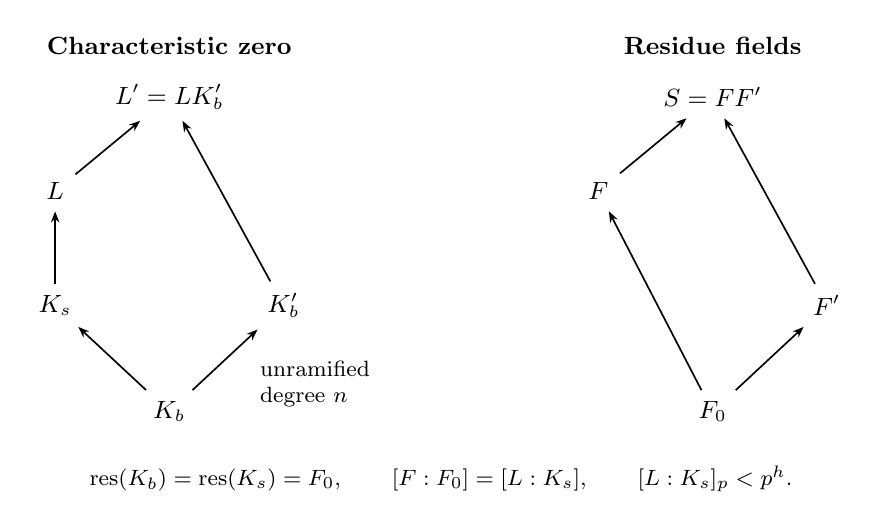
\begin{tikzpicture}[
  every node/.style={font=\small},
  field/.style={inner sep=4pt},
  inclusion/.style={-{Stealth[length=4pt]},semithick}
]
\begin{scope}[xshift=-3.45cm]
  \node[font=\small\bfseries] at (0,4.65) {Characteristic zero};
  \node[field] (kb) at (0,0) {$K_b$};
  \node[field] (ks) at (-1.45,1.35) {$K_s$};
  \node[field] (kbp) at (1.45,1.35) {$K_b'$};
  \node[field] (l) at (-1.45,2.8) {$L$};
  \node[field] (lp) at (0,4) {$L'=LK_b'$};
  \draw[inclusion] (kb)--(ks);
  \draw[inclusion] (kb)--(kbp);
  \node[font=\footnotesize,align=left] at (1.85,.35)
    {unramified\\degree $n$};
  \draw[inclusion] (ks)--(l);
  \draw[inclusion] (l)--(lp);
  \draw[inclusion] (kbp)--(lp);
\end{scope}
\begin{scope}[xshift=3.45cm]
  \node[font=\small\bfseries] at (0,4.65) {Residue fields};
  \node[field] (f0) at (0,0) {$F_0$};
  \node[field] (fp) at (1.45,1.35) {$F'$};
  \node[field] (f) at (-1.45,2.8) {$F$};
  \node[field] (s) at (0,4) {$S=FF'$};
  \draw[inclusion] (f0)--(fp);
  \draw[inclusion] (f0)--(f);
  \draw[inclusion] (f)--(s);
  \draw[inclusion] (fp)--(s);
\end{scope}
\node[font=\footnotesize,align=center] at (0,-.85)
 {$\operatorname{res}(K_b)=\operatorname{res}(K_s)=F_0,
   \qquad [F:F_0]=[L:K_s],\qquad [L:K_s]_p<p^h.$};
\end{tikzpicture}
\caption{The auxiliary fields in a descent arising from a small Sylow orbit. Arrows denote field inclusions. The right-hand diagram records the residues of the left-hand fields; in particular $K_b$ and $K_s$ have the same residue. The field $K_b'$ splits the marked sections, and its residue $F'$ splits their reductions. The cyclic extension $K_b'/K_b$ reduces to $F'/F_0$, and the Galois actions of $L'/L$ and $S/F$ induce the same permutations of the marked points.}
\label{fig:field-tower}
\end{figure}


\section{Specialization, connectedness, and the tuple count}\label{sec:specialization}

We retain the auxiliary fields and marked genus-one curve constructed in
\Cref{prop:mixed-lift,prop:spherical-base}. In this section $m=|J|$, $h\geq1$,
and $n=p^s$. Choose $s$ so that
\begin{equation}\label{eq:specialization-threshold}
 s\geq\max\{1,h\},\qquad
 p^{s-h}>m\bigl(h+\log_p m\bigr).
\end{equation}
This is a sufficient threshold for \Cref{thm:inseparable-genus}.
The relatively ample effective divisor $D$ has degree $n$ on each fiber
and is disjoint from the marked sections after their splitting extension.

\begin{proposition}\label{prop:no-small-cover}
Suppose $O_p(J)=1$ and \eqref{eq:specialization-threshold} holds. There is no
finite extension $L/K_s$ with $[L:K_s]_p<p^h$ over which the marked curve
$X=\mathcal X_L$ admits a geometrically connected smooth projective
$J$-Galois cover $f:Y\to X$, with its $J$-action defined over $L$, branched
only at the marked points and with ramification index divisible by $p$ at
every marked point.
\end{proposition}

We will obtain the contradiction by producing a nontrivial normal
$p$-subgroup of $J$. To this end, we first extract residue curves from
one $J$-orbit of valuations of a supposed cover. A comparison of
sections determines their total degree. A second comparison, with
prescribed vanishing, combines with the genus estimates to force
equality of Euler characteristics. These two equalities yield a flat
model whose special fiber is the disjoint union of those residue curves.
Connectedness will force the orbit to have one member; the kernel of
the resulting $J$-action on its residue field will be the required
nontrivial normal $p$-subgroup.

Suppose, for the proof, that such a cover exists. Its smooth,
geometrically connected source $Y$ is geometrically integral: over an
algebraic closure, the irreducible components of a smooth curve are
disjoint, so connectedness leaves only one. Let $R$ be the valuation
ring of $L$, with maximal ideal $\mathfrak m_R$ and residue field $F$.
By \Cref{prop:spherical-base}, $L$ is spherically complete, its value group
is $\mathbb Q$, and
\[
 [F:F_0]_p=[L:K_s]_p<p^h.
\]
Put $L'=LK_b'$ and $S=FF'$. By \Cref{lem:residue-permutations}, $S$ is the
residue field of $L'$, and the permutation actions on the labels $\xi_i$
over $L'$ and $t_i$ over $S$ agree. Write $D_X$ and $D_F$ for the divisors
induced by $D$ on $X$ and $E_F$, respectively, and put $D_Y=f^*D_X$.
The field extension $L(Y)/L(X)$ is Galois of degree $m$, with group $J$:
these assertions hold after extension to an algebraic closure, and the
specified automorphisms are already defined over $L$.

Let $e_i$ be the geometric ramification index at $\xi_i$. Each $e_i$ is
divisible by $p$. Riemann--Hurwitz over an algebraic closure, together
with invariance of Euler characteristic under field extension, gives
\begin{equation}\label{eq:generic-hurwitz}
 \frac{\nu(Y)}m
 =\frac{-2\chi(Y)}m
 =\sum_{i=1}^n\left(1-\frac1{e_i}\right).
\end{equation}
Here the base has genus one, and the reduced geometric fiber above
$\xi_i$ consists of $m/e_i$ points. The characteristic-zero form of
Riemann--Hurwitz being used is included in \Cref{foundation:complex}.

\subsection{The Gauss valuation and reduction of sections}

\begin{lemma}\label{lem:gauss-section-rule}
There is a valuation $v_X$ on $L(X)$ extending that on $L$, with value
group $\mathbb Q$ and residue field $F(E_F)$, having the following
properties. For every sufficiently large $j$, the integral ball in
$H^0(X,\mathcal O_X(jD_X))$ reduces onto
$H^0(E_F,\mathcal O_{E_F}(jD_F))$. Reduction is compatible with inclusions
as $j$ increases and with multiplication. Moreover, for an integral
section $b$ in such a space,
\begin{equation}\label{eq:gauss-evaluation}
 \overline{b(\xi_i)}=\bar b(t_i)
 \qquad\text{in }S.
\end{equation}
In particular, vanishing at $\xi_i$ implies vanishing of its reduction
at $t_i$.
\end{lemma}

\begin{proof}
Work initially over the complete DVR $R_b$, and write $D_E=D|_E$.
For $j$ sufficiently large,
\Cref{foundation:cohomology} and the special-fiber sequence give
\[
 H^0(\mathcal X,\mathcal O(jD))\otimes_{R_b}F_0
 \simeq H^0(E,\mathcal O_E(jD_E)).
\]
Indeed Serre vanishing kills $H^1(\mathcal X,\mathcal O(jD))$, so the
sequence obtained by multiplication by a uniformizer gives surjectivity
onto the special sections. The module on the left before reduction is
finite and torsion-free, hence free over $R_b$; torsion-freeness follows
from flatness of $\mathcal X$ and invertibility of $\mathcal O(jD)$.
Choose a basis $b_{j,1},\ldots,b_{j,t_j}$ whose reductions are a basis
of the special section space. Flat base change supplies bases over $L$
on the generic side and over $F$ on the special side.

As $D_X$ is effective, regard these sections as rational functions.
For $b=\sum_\alpha c_\alpha b_{j,\alpha}$ put
\[
 v_X(b)=\min_\alpha v(c_\alpha).
\]
Integral coefficients give a special rational function with poles
bounded by $jD_F$, and this function is nonzero if the displayed minimum
is zero. The inclusions for $jD\leq j'D$ are integral maps on the original
model and reduce to injective inclusions of special section spaces.
Consequently the assigned value is independent of the sufficiently
large space containing $b$: scale the coefficients so that their minimum
is zero, and use the nonzero special image. The same argument proves
multiplicativity. After scaling two nonzero sections to value zero, their
reductions are nonzero, and their product is nonzero because $E_F$ is
integral. The strong triangle inequality follows directly from the
coefficient rule.

The union of these section spaces is a ring whose fraction field is
$L(X)$: sufficiently high ample multiples give a projective embedding,
and their section ratios generate the function field. Thus the rule
extends to a valuation on $L(X)$. Its values lie in $\mathbb Q$, and all
values in $\mathbb Q$ occur already on $L$. A fraction of value zero can
be written with numerator and denominator both of value zero, by a
common scalar rescaling. Its residue is the ratio of their nonzero
special reductions, hence lies in $F(E_F)$. Conversely the ratios of
high-degree special sections generate $F(E_F)$, and each such section
has an integral lift. This identifies the residue field.

Finally the basis functions are regular along the splitting sections
over $R_b'$, since those sections avoid $D$. Their values are integral
and reduce to their evaluations at $t_i$. The same holds after extension
of coefficients from $R_b$ to $R$ and evaluation over the valuation ring
of $L'$. Since its residue is $S$, this proves
\eqref{eq:gauss-evaluation}.
\end{proof}

Choose one prolongation of $v_X$ to $L(Y)$, and let $\mathcal V$ be its
orbit of distinct conjugates under $J$. For $w\in\mathcal V$ let $K(w)$
be its residue field. The single-place residue-degree bound in
\Cref{lem:simultaneous-residues} makes $K(w)/F(E_F)$ finite; the Gauss
valuation has value group $\mathbb Q$ and infinite residue field $F(E_F)$.
Set
\[
 m_w=[K(w):F(E_F)].
\]
Let $C_w$ be the normalization of $E_F$ in $K(w)$ and $D_w$ the pullback
of $D_F$. These are regular integral projective curves, with finite
maps to $E_F$, by \Cref{foundation:normalization}.
Throughout the next argument we use this single orbit; its size is not
assumed in advance to account for all the extension degree.

For $j\geq0$ put
\[
 V_j=H^0(Y,\mathcal O_Y(jD_Y)),\qquad
 v_{\mathcal V}(a)=\min_{w\in\mathcal V}w(a),\qquad
 A_j=\{a\in V_j:v_{\mathcal V}(a)\geq0\}.
\]
The minimum is a valuation norm on the $L$-vector space $V_j$.
All prolongation values lie in $\mathbb Q$: algebraicity makes the
extension of value groups torsion, while the base value group is
divisible. The orthogonal-basis assertion of \Cref{lem:orthogonal-bases}
therefore applies, and an orthogonal basis can be scaled to have value
zero. In this basis,
\begin{equation}\label{eq:section-lattice}
 A_j\simeq R^{\dim_L V_j},\qquad
 \{a\in V_j:v_{\mathcal V}(a)>0\}=\mathfrak m_R A_j.
\end{equation}
These assertions also hold on any $L$-linear subspace of $V_j$.
At this point reduction means the map of rational functions
\[
 A_j\longrightarrow\prod_{w\in\mathcal V}K(w),
 \qquad a\longmapsto(\bar a_w)_w.
\]
Its kernel is the positive ball $\mathfrak m_R A_j$, so its image
has dimension $\dim_L V_j$ over $F$. No model of $Y$ has been used.
The next lemma locates these residue-field elements in the section
spaces of the separately normalized curves $C_w$.

\begin{lemma}\label{lem:section-specialization}
For all sufficiently large $j$, simultaneous residue gives an injection
\begin{equation}\label{eq:section-reduction}
 A_j/\mathfrak m_R A_j
 \lhook\joinrel\longrightarrow
 \bigoplus_{w\in\mathcal V}
 H^0(C_w,\mathcal O_{C_w}(jD_w)).
\end{equation}
These maps respect products. If a section vanishes on the reduced
inverse images of a selected set of marked points, its reductions
vanish on the corresponding reduced inverse images on the $C_w$,
provided the selections are defined over the respective ground fields.
The vanishing assertion may be checked after splitting the marked
points over $L'$ and $S$.
\end{lemma}

\begin{proof}
Let $a\in A_j$. Form the polynomial using every element of $J$,
including any repeated conjugates:
\begin{equation}\label{eq:conjugate-section-polynomial}
 P_a(T)=\prod_{g\in J}(T-g(a))
       =T^m+c_1T^{m-1}+\cdots+c_m.
\end{equation}
The coefficients are $J$-invariant rational functions, hence belong to
$L(Y)^J=L(X)$. At a fixed $w\in\mathcal V$ every
$g(a)$ is integral, because $g$ permutes $\mathcal V$. Thus each $c_k$
has nonnegative Gauss value. Moreover
\[
 c_k\in H^0(X,\mathcal O_X(kjD_X)).
\]
To see the pole bound, each conjugate has poles bounded by $jD_Y$, so
the elementary symmetric function of degree $k$ has poles bounded by
$kjD_Y$. Since the coefficient is a rational function on $X$, its
pole bound on $X$ follows from that on its finite surjective pullback.

By \Cref{lem:gauss-section-rule}, $\bar c_k$ has poles bounded by
$kjD_F$. The residue $\bar a_w\in K(w)$ satisfies the reduction of
\eqref{eq:conjugate-section-polynomial}. Let $t$ be a local equation for
$jD_F$ at any point of $E_F$. Then $t\bar a_w$ satisfies the monic
equation whose coefficient of degree $m-k$ is $t^k\bar c_k$.
These coefficients are regular there. At every point of $C_w$ above
this neighborhood, normality therefore makes $t\bar a_w$ regular.
This proves the required pole bound and hence
\eqref{eq:section-reduction}; injectivity was established in
\eqref{eq:section-lattice}. Residue maps themselves respect multiplication.

For the last assertion, work at a selected marked point after splitting.
Every $g(a)$ vanishes at every point of its reduced inverse fiber,
because this fiber is $J$-invariant. The non-leading coefficients
$c_k$ consequently vanish at the marked point downstairs. There are
no poles there, since $D_X$ avoids all the marked points.
By \eqref{eq:gauss-evaluation}, every $\bar c_k$ vanishes at $t_i$.
The reduced monic equation at any point above $t_i$ is then
$\bar a_w^m=0$ in its residue field, so $\bar a_w$ vanishes there.
\end{proof}

\subsection{Residue degrees and the inseparable quotient}

For $j$ sufficiently large, the line-bundle Euler-characteristic formula
and ample vanishing turn \eqref{eq:section-reduction} into
\begin{equation}\label{eq:full-section-comparison}
 jmn+\chi(Y)
 \leq jn\sum_{w\in\mathcal V}m_w
       +\sum_{w\in\mathcal V}\chi(C_w).
\end{equation}
Here $\deg D_X=\deg D_F=n$, and finite pullback multiplies divisor
degree by the map degree. Letting $j$ grow gives
$m\leq\sum_wm_w$. On the other hand,
\Cref{lem:simultaneous-residues}, applied to the Gauss valuation on
$L(X)$ and these distinct prolongations to the degree-$m$ extension
$L(Y)$, gives the reverse inequality. Its hypotheses hold: the value
group is $\mathbb Q$ and the residue field $F(E_F)$ is infinite.
We have proved
\begin{equation}\label{eq:residue-degree-equality}
 \sum_{w\in\mathcal V}m_w=m.
\end{equation}

Let $\Delta_w\leq J$ be the stabilizer of $w$, and let $I_w$ be the
kernel of its action on $K(w)$. The orbit has $m/|\Delta_w|$ members,
all of the same residue degree. Therefore
\begin{equation}\label{eq:decomposition-residue-degree}
 m_w=|\Delta_w|.
\end{equation}
In particular this equality follows from the section comparison, before
any assertion about the degree of an inseparable quotient.

\begin{lemma}\label{lem:inseparable-residue-quotient}
The invariant field $M_w=K(w)^{\Delta_w}$ is purely inseparable over
$F(E_F)$, of degree
\begin{equation}\label{eq:inertia-inseparable-degree}
 d=[M_w:F(E_F)]=|I_w|.
\end{equation}
In particular $d$ is a power of $p$ and $d\leq m$. If $Z_w$ denotes the
normalization of $E_F$ in $M_w$, the map $C_w\to Z_w$ is generically
separable Galois of degree $m_w/d$, with group $\Delta_w/I_w$.
All these towers are isomorphic over $E_F$ as $w$ varies in $\mathcal V$.
\end{lemma}

\begin{proof}
Take $x\in K(w)^{\Delta_w}$. Simultaneous approximation from
\Cref{lem:simultaneous-residues} gives an element $a\in L(Y)$ integral
at every member of $\mathcal V$, with residue $x$ at $w$ and zero at
the other members. The coefficients of the conjugate polynomial
$P_a(T)$ in \eqref{eq:conjugate-section-polynomial} have nonnegative
Gauss value. At $w$, its reduction is
\begin{equation}\label{eq:invariant-residue-polynomial}
 \overline{P_a}(T)
 =T^{m-|\Delta_w|}(T-x)^{|\Delta_w|}
 \in F(E_F)[T].
\end{equation}
Indeed, elements of $\Delta_w$ act on the residue $x$ trivially, and
each other conjugate draws its residue from a different member of
the orbit, where the prescribed residue is zero.

Write $|\Delta_w|=p^v q$ with $p\nmid q$. In characteristic $p$,
\[
 (T-x)^{|\Delta_w|}=(T^{p^v}-x^{p^v})^q.
\]
The coefficient of $T^{m-p^v}$ in
\eqref{eq:invariant-residue-polynomial} is therefore
$-q x^{p^v}$. The scalar $q$ is nonzero in $F(E_F)$, so
$x^{p^v}\in F(E_F)$. This also covers $x=0$, for which the coefficient
is zero. Thus $M_w/F(E_F)$ is purely inseparable.

The effective automorphism group on $K(w)$ is $\Delta_w/I_w$.
Finite fixed-field theory gives
\[
 [K(w):M_w]=|\Delta_w/I_w|.
\]
Combining this with \eqref{eq:decomposition-residue-degree} and the
tower formula proves \eqref{eq:inertia-inseparable-degree}.
The assertions about the normalizations and their separable function
fields follow. Conjugation by $J$ supplies the asserted isomorphisms
between the towers, so $d$ is independent of $w$.
\end{proof}

\subsection{Ramification on the residue curves}

Pass temporarily to the finite separable splitting field $S/F$.
The curve $Z_{w,S}$ remains integral: its finite map to $E_S$ is
surjective and radicial, while separable scalar extension preserves
regularity and hence reducedness. The curve $C_{w,S}$ is regular and
is a disjoint union of integral components. Each component dominates
$Z_{w,S}$: the finite flat map $C_{w,S}\to Z_{w,S}$ restricts on a
component to a nonzero finite locally free summand, of positive rank
on the connected target. The components are consequently the
normalizations in their respective function fields. These uses of
normalization and separable scalar extension are included in
\Cref{foundation:normalization,foundation:regularity}.

Let $z_i$ be the unique point of $Z_{w,S}$ above $t_i$, and write $r_i$
for its ramification index over $t_i$. Write $a_i$ for the ramification
index of $C_{w,S}\to Z_{w,S}$ above $z_i$. We justify that $a_i$ is
independent of the point above $z_i$, even when $C_{w,S}$ is disconnected.
Put $G_w=\Delta_w/I_w$ and $M_{w,S}=S(Z_{w,S})$. The generic algebra
of this map is
\[
 K(w)\otimes_{M_w}M_{w,S}=\prod_{\lambda=1}^t K_\lambda.
\]
It is a product of fields because $K(w)/M_w$ is finite separable.
The group $G_w$ acts on the first tensor factor, and the invariant
algebra is $M_{w,S}$: taking invariants is taking a kernel of linear
maps, which commutes with this scalar extension. An orbit of the
field factors gives an invariant idempotent. Since $M_{w,S}$ is a
field, there can be only one orbit.

The total dimension over $M_{w,S}$ is $|G_w|$, and transitivity makes
all factor degrees equal to $|G_w|/t$. The stabilizer of a factor has
this same order. It acts faithfully on that factor, since the map
from $K(w)$ into the factor is injective. Thus the factor extension
is Galois with that stabilizer as its group. Transitivity on primes
in each Galois normalization gives transitivity within each component
above $z_i$; the action on the factors joins these componentwise
orbits. We obtain transitivity on the entire fiber of $C_{w,S}$.
Ramification indices are preserved by this action. The isomorphisms
between the towers for different $w$ give the same $r_i,a_i$ throughout
the orbit.

Multiplicities in the tower multiply, so every point $P$ of $C_{w,S}$
above $t_i$ has index $r_i a_i$ over $t_i$. Finite flatness gives
\[
 \sum_{P\in C_{w,S},\ P\mid t_i}
    r_i a_i\,[\kappa(P):S]=m_w.
\]
Summing over $w$ and using \eqref{eq:residue-degree-equality} yields
\begin{equation}\label{eq:reduced-special-fiber-degree}
 \sum_{w\in\mathcal V}\ 
 \sum_{P\in C_{w,S},\ P\mid t_i}[\kappa(P):S]
 =\frac{m}{r_i a_i}.
\end{equation}
In particular all residue-field degrees, including inseparable ones,
are retained in the degree of the reduced fiber.

Apply \Cref{lem:separable-different} to $C_{w,S}\to Z_{w,S}$,
component by component. At a point above $z_i$, the determinant
vanishing is at least
$a_i-1+\mathbf 1_{p\mid a_i}$. The total separable degree of the
components over $Z_{w,S}$ is $m_w/d$. The preceding local-degree
calculation gives $m_w/(r_i a_i)$ for the sum of the full residue-field
degrees above $t_i$. Hence, for each $w$,
\[
 \nu(C_w)\geq\frac{m_w}{d}\nu(Z_w)
 +\sum_{i=1}^n\frac{m_w}{r_i a_i}
       \bigl(a_i-1+\mathbf 1_{p\mid a_i}\bigr).
\]
Euler characteristics and divisor degrees have the same numerical
values over $F$ as after the separable extension to $S$, so this
inequality is written in the original normalization over $F$.
The hypotheses of
\Cref{thm:inseparable-genus} hold for $Z_w/E_F$:
$[F:F_0]_p<p^h$, and \Cref{lem:inseparable-residue-quotient} gives
a purely inseparable degree $d\leq m$. Divide the displayed inequality
by $m_w$ and substitute that theorem's bound for $\nu(Z_w)/d$.
Now sum with weights $m_w/m$, whose sum is one by
\eqref{eq:residue-degree-equality}. This gives
\begin{equation}\label{eq:residue-genus}
 \frac{\sum_{w\in\mathcal V}\nu(C_w)}m
 \geq
 \sum_{i=1}^n\left(1-\frac1{r_i}\right)
 +\sum_{i=1}^n
   \frac{a_i-1+\mathbf 1_{p\mid a_i}}{r_i a_i}.
\end{equation}
Thus the normalization in this inequality agrees with that of
\eqref{eq:generic-hurwitz}.

\subsection{Vanishing conditions force equality}

The ramification estimate \eqref{eq:residue-genus} involves the
special indices $r_i a_i$, whereas \eqref{eq:generic-hurwitz}
involves the generic indices $e_i$. A second comparison of section
spaces will control their difference. Choose the labels in the set
\[
 \mathcal I=\left\{i:\frac1{r_i a_i}>\frac1{e_i}\right\}.
\]
At these labels, the degree $m/(r_i a_i)$ of the reduced special fiber
exceeds the degree $m/e_i$ of the reduced generic fiber. Imposing
vanishing there will make the section comparison detect this excess.
This selection descends on both sides. The generic index $e_i$ is
constant on the label orbits of $\operatorname{Gal}(L'/L)$, and the
special indices $r_i,a_i$ are constant on the label orbits of
$\operatorname{Gal}(S/F)$. These two permutation actions agree by
\Cref{lem:residue-permutations}. Hence the same subset of labels
defines a divisor over $L$ on the generic base and a divisor over $F$
on the special base.

Let $T_Y$ be the reduced inverse image on $Y$ of this selected divisor,
and let $T_w$ be its counterpart on $C_w$. These are effective divisors
on regular curves over their indicated fields. Their degrees may be
computed after the finite separable splitting extensions, which preserve
reducedness. The generic Galois cover and
\eqref{eq:reduced-special-fiber-degree} give
\begin{equation}\label{eq:selected-divisor-degrees}
 \deg_L T_Y=\sum_{i\in\mathcal I}\frac m{e_i},\qquad
 \sum_{w\in\mathcal V}\deg_F T_w
    =\sum_{i\in\mathcal I}\frac m{r_i a_i}.
\end{equation}

Restrict the norm to
$H^0(Y,\mathcal O_Y(jD_Y-T_Y))$. Its integral ball again has a
full-dimensional reduction by \eqref{eq:section-lattice}, and
\Cref{lem:section-specialization} places that reduction in
\[
 \bigoplus_{w\in\mathcal V}
 H^0(C_w,\mathcal O_{C_w}(jD_w-T_w)).
\]
For sufficiently large $j$, ample vanishing and
\eqref{eq:residue-degree-equality} therefore give
\[
 jmn+\chi(Y)-\deg_L T_Y
 \leq jmn+\sum_w\chi(C_w)-\sum_w\deg_F T_w.
\]
After rearranging and using \eqref{eq:selected-divisor-degrees}, this is
\begin{equation}\label{eq:vanishing-comparison}
 \frac{\nu(Y)}m
 \geq \frac{\sum_{w\in\mathcal V}\nu(C_w)}m
 +2\sum_{i=1}^n
   \max\left\{\frac1{r_i a_i}-\frac1{e_i},0\right\}.
\end{equation}

The three comparisons now force equality. To display their exact
interaction, put
\[
 q_i=\frac1{r_i a_i},\qquad b_i=\frac1{e_i},\qquad
 \delta_i=\mathbf 1_{p\mid a_i}.
\]
The contribution of label $i$ in \eqref{eq:residue-genus} is
$1-q_i+\delta_iq_i$. Combining that inequality with
\eqref{eq:vanishing-comparison} and subtracting
\eqref{eq:generic-hurwitz} gives
\begin{align}
 0
 &\geq \sum_{i=1}^n
       \bigl(b_i-q_i+2\max\{q_i-b_i,0\}+\delta_iq_i\bigr)
       \notag\\
 &=\sum_{i=1}^n\bigl(|q_i-b_i|+\delta_iq_i\bigr)
 \geq0.\label{eq:genus-nonnegative-excess}
\end{align}
Every summand vanishes, and every intervening inequality is an equality.
In particular,
\begin{equation}\label{eq:sharp-specialization}
 r_i a_i=e_i,\qquad p\nmid a_i\quad(1\leq i\leq n),
 \qquad d=|I_w|>1,
 \qquad \chi(Y)=\sum_{w\in\mathcal V}\chi(C_w).
\end{equation}
For the strict inequality $d>1$, use $p\mid e_i$ and $p\nmid a_i$:
then $r_i>1$, and $r_i$ divides the purely inseparable degree $d$ by
finite flatness at $t_i$. Also $q_i=b_i$ makes the extra term in
\eqref{eq:vanishing-comparison} zero, so equality there gives precisely
the displayed Euler-characteristic equality.

\subsection{A finitely presented model over the valuation ring}

\begin{proposition}\label{prop:specialization-model}
The degree equality \eqref{eq:residue-degree-equality} and the
Euler-characteristic equality in \eqref{eq:sharp-specialization}
produce a flat projective scheme $\mathcal Y$ of finite presentation
over $R$, with
\[
 \mathcal Y_L\simeq Y,\qquad
 \mathcal Y_F\simeq\coprod_{w\in\mathcal V}C_w.
\]
\end{proposition}

\begin{proof}
Form the graded $R$-algebra
\[
 A=\bigoplus_{j\geq0}A_j.
\]
Multiplication is defined because each $w$ is a valuation:
$A_iA_j\subseteq A_{i+j}$. Each piece is finite free by
\eqref{eq:section-lattice}. Moreover $A_0=R$, since $Y$ is projective
and geometrically integral and hence $H^0(Y,\mathcal O_Y)=L$.
Put
\[
 C=\coprod_{w\in\mathcal V}C_w,
 \qquad B_j=\bigoplus_{w\in\mathcal V}
 H^0(C_w,\mathcal O_{C_w}(jD_w)),
 \qquad B=\bigoplus_{j\geq0}B_j.
\]
The two equalities in the proposition make the source and target
dimensions in \eqref{eq:section-reduction} equal for every sufficiently
large $j$. Thus there is an integer $j_0$ such that
\begin{equation}\label{eq:full-high-degree-reduction}
 A_j/\mathfrak m_R A_j\simeq B_j
 \qquad(j\geq j_0),
\end{equation}
compatibly with products. Equality in each high degree, rather than
only equality of leading terms, is where the Euler-characteristic
equality is used.

We first choose a Veronese regrading for which the reduced algebra is
generated in degree one. The divisor on $C$ given by the $D_w$ is ample,
so $B$ is finitely generated by \Cref{foundation:cohomology}. Choose
positive-degree homogeneous generators $b_1,\ldots,b_t$ over $B_0$,
of degrees $d_1,\ldots,d_t$. Let $W$ be a common multiple of these
positive degrees. In a monomial in the $b_i$, remove pure powers
$b_i^{W/d_i}$, each of weight $W$, until the remaining exponent of
$b_i$ is less than $W/d_i$. The weight of the remainder is less than
$tW$. Choose $N=qW\geq j_0$ with $q\geq t$.

If the original monomial has degree $kN$, its remainder has weight
$cW$ for an integer $0\leq c<t\leq q$, since the removed blocks
and the original total weight are multiples of $W$. There are
$kq-c$ removed blocks. Combine the remainder with $q-c$ of these
blocks to make one factor of weight $N$, and group the remaining
$(k-1)q$ blocks in groups of $q$. This factors the monomial into
$k$ factors of weight $N$. Any coefficient from $B_0$ is absorbed
into the first factor. It follows that
\begin{equation}\label{eq:special-veronese-generation}
 F\ \oplus\!\bigoplus_{k\geq1} B_{kN}
 \quad\text{is generated over $F$ by }B_N.
\end{equation}
This argument permits $B_0=H^0(C,\mathcal O_C)$ to be larger than
$F$, as can happen for a disconnected curve or a curve with extra
constants. All the positive-degree factors used in the argument
belong to the full spaces in \eqref{eq:full-high-degree-reduction}.

Let $A^{(N)}=\bigoplus_{k\geq0}A_{kN}$, with $A_{kN}$ assigned degree
$k$. Choose an $R$-basis of $A_N$, and map the variables of a
degree-one polynomial ring
\[
 P=R[x_1,\ldots,x_u]\longrightarrow A^{(N)}
\]
to that basis. In each degree the target is a finite free $R$-module.
By \eqref{eq:full-high-degree-reduction} and
\eqref{eq:special-veronese-generation}, the map is surjective after
reduction modulo $\mathfrak m_R$. Its degreewise cokernel is finite,
so Nakayama's lemma makes the map surjective in every degree.
This proves finite generation over $R$.

For finite presentation, let $K_k$ be the kernel of
$P_k\to A_{kN}$. This surjection splits as an $R$-module map because
$A_{kN}$ is free. Hence $K_k$ is a finite direct summand of the finite
free module $P_k$, and reduction gives the exact kernel of the
corresponding polynomial presentation over $F$. The special relation
ideal is a homogeneous ideal in the Noetherian ring
$F[x_1,\ldots,x_u]$, so it has finitely many homogeneous generators.
Lift them, in their respective degrees, to elements $g_1,\ldots,g_v$
of $\ker(P\to A^{(N)})$, and let $I$ be the ideal they generate.
For every $k$, the quotient $K_k/I_k$ is a finite $R$-module. Its
reduction is zero, since the reductions of the $g_i$ generate the
special relation ideal. Degreewise Nakayama gives $K_k=I_k$ for every
$k$. Thus
\[
 A^{(N)}\simeq R[x_1,\ldots,x_u]/(g_1,\ldots,g_v)
\]
is a finite homogeneous presentation. In particular, this argument
does not require the nondiscrete valuation ring $R$ to be Noetherian.

Define $\mathcal Y=\operatorname{Proj}A^{(N)}$. The degree-one
presentation makes it a projective $R$-scheme of finite presentation.
It is flat over $R$: the graded algebra is a direct sum of free
$R$-modules, homogeneous localization is a filtered colimit of such
flat modules, and the degree-zero part of the resulting graded module
is a direct summand. Thus every standard affine chart of $\mathcal Y$
has a flat coordinate ring over $R$.

Since $A_j$ spans $V_j$, the generic fiber is the Proj of the ample
section ring of $Y$ after Veronese regrading, and hence is $Y$.
By \eqref{eq:full-high-degree-reduction}, the special fiber is the
Proj of the algebra in \eqref{eq:special-veronese-generation}.
Replacing its degree-zero term $F$ by $B_0$ has no effect on Proj.
Indeed, on a localization at a positive-degree element $f$, a missing
constant $b\in B_0$ is present as $(bf)/f$, since $bf$ has positive
degree. The degree-zero coordinate rings of these localizations
therefore agree. The full ample section ring recovers $C$, proving
the special-fiber assertion.
\end{proof}

\subsection{Connectedness and the final contradiction}

The finite presentation just proved is what permits passage to a
Noetherian base. This is the finite-equation approximation framework
of EGA IV \cite[Section~8]{EGAIV3}; the connected-fiber input is Stein
factorization, as in EGA III \cite[Section~4.3]{EGAIII1} and
\Cref{foundation:connectedness}. The following argument constructs
the normal Noetherian base explicitly, rather than applying coherent
finiteness or Stein factorization to the original valuation ring.

\begin{lemma}\label{lem:valuation-model-connectedness}
Let $R$ be a valuation ring of a characteristic-zero field $L$.
If a flat projective $R$-scheme $\mathcal U$ of finite presentation
has geometrically integral generic fiber, then its special fiber
is geometrically connected.
\end{lemma}

\begin{proof}
Choose a finite set of homogeneous projective equations for
$\mathcal U$. Their coefficients generate a finite-type
$\mathbb Z$-subdomain $R_0\subset R$. Normalize $R_0$ in its fraction
field, obtaining $R_1$. By \Cref{foundation:normalization}, this
normalization is finite, so $R_1$ is a normal Noetherian domain.
It remains a subring of $R$: its elements lie in $\operatorname{Frac}(R_0)$
and are integral over $R$, which is integrally closed.

The equations define a projective scheme $\mathcal U_1$ over $R_1$.
Its generic fiber is geometrically integral, because this can be
checked after extension of its fraction field to $L$, where the
fiber is $\mathcal U_L$. Let $\mathcal T\subseteq\mathcal U_1$ be the
scheme-theoretic closure of that generic fiber. Then $\mathcal T$ is
integral and projective over $R_1$: locally its coordinate ring is
the image in the coordinate ring of the integral generic fiber,
and the generic fiber is dense.

The pullback $\mathcal T_R$ is a closed subscheme of $\mathcal U$ and
agrees with it over $L$. Its defining ideal in
$\mathcal O_{\mathcal U}$ therefore vanishes upon localization at
$R\setminus\{0\}$. On each affine chart, every element of this ideal
is annihilated by a nonzero element of $R$. Flatness of $\mathcal U$
makes its affine coordinate rings torsion-free over $R$, so the ideal
is already zero. Thus
\begin{equation}\label{eq:normal-approximation-pullback}
 \mathcal T_R=\mathcal U.
\end{equation}

Write $K_1=\operatorname{Frac}(R_1)$ and
$\pi:\mathcal T\to\operatorname{Spec}R_1$.
Proper coherent finiteness over this Noetherian base gives a finite
$R_1$-algebra $H^0(\mathcal T,\mathcal O_{\mathcal T})$.
Restriction to the generic fiber is injective because $\mathcal T$
is integral and that fiber is dense. Since the generic fiber is
projective and geometrically integral, its global functions are
$K_1$. Hence
\[
 R_1\subseteq H^0(\mathcal T,\mathcal O_{\mathcal T})\subseteq K_1.
\]
The middle ring is finite over $R_1$, so all its elements are integral
over $R_1$. Normality yields
$H^0(\mathcal T,\mathcal O_{\mathcal T})=R_1$. Equivalently,
\[
 \pi_*\mathcal O_{\mathcal T}=\mathcal O_{\operatorname{Spec}R_1};
\]
one can check this equality on principal affine opens by flat base
change for coherent cohomology, as in \Cref{foundation:cohomology}.

Stein connectedness over the Noetherian base, in the form stated in
\Cref{foundation:connectedness}, now gives geometrically connected
fibers of $\pi$. The special fiber of $\mathcal U$ is, by
\eqref{eq:normal-approximation-pullback}, an extension of one of these
fibers to the residue field of $R$. It is therefore geometrically
connected. All uses of proper coherent cohomology and Stein
factorization in this proof occur over $R_1$.
\end{proof}

\begin{proof}[Completion of the proof of \Cref{prop:no-small-cover}]
Apply \Cref{lem:valuation-model-connectedness} to the flat projective
model of \Cref{prop:specialization-model}. Its generic fiber $Y$ is
geometrically integral, so its special fiber
$\coprod_{w\in\mathcal V}C_w$ is connected. Every $C_w$ is nonempty;
hence $\mathcal V$ has one member. The stabilizer of that member is
all of $J$, so $I_w$ is a normal subgroup of $J$. By
\eqref{eq:inertia-inseparable-degree} and
\eqref{eq:sharp-specialization}, it is a nonidentity $p$-group.
This contradicts $O_p(J)=1$.
\end{proof}

\begin{proof}[Proof of \Cref{thm:tuple-divisibility}]
Fix $h\geq1$ and choose $s_0$ satisfying
\eqref{eq:specialization-threshold} with $s=s_0$.
The same inequalities hold for every $s\geq s_0$; fix any such $s$.
For any prescribed multiset of
conjugacy classes of the $p$-singular puncture entries,
\Cref{lem:marked-cover-classification,prop:small-orbit-descent}
identify the finite tuple-class set with the corresponding marked-cover
classes and supply a Sylow
$p$-group action on that set. If an orbit had size less than $p^h$,
the same proposition would descend one of its covers to a finite
extension $L/K_s$ with $[L:K_s]_p<p^h$. This is excluded by
\Cref{prop:no-small-cover}.

Every orbit of a finite $p$-group has $p$-power size. Thus all the
orbits have sizes divisible by $p^h$, and so does their total.
The threshold depends only on $p,h,m$, not on the multiset.
An empty tuple set has count zero and satisfies the same assertion;
in particular this covers groups with no $p$-singular elements.
\end{proof}

\begin{proof}[Proof of \Cref{thm:main}]
The tuple divisibility just proved supplies the hypothesis of
\Cref{prop:group-reduction}. Therefore $l=(1+T)z$ for every pair
$(X,E)$ of a finite group and a central block sum considered there.
Taking $(X,E)=(G,B)$ gives
\[
 l(B)=
 \sum_{\substack{Q\leq G\text{ a }p\text{-subgroup}\\
                   \text{up to }G\text{-conjugacy}}}
 z\bigl(N_G(Q)/Q,\bar B_Q\bigr).
\]
The normalizer block-assignment calculation following
\Cref{lem:normalizer-projection} identifies this sum, including $Q=1$,
with $|W_p(B)|$ under the central-character convention
\eqref{eq:block-assignment}. Hence $l(B)=|W_p(B)|$ for every prime,
finite group, and block, as required.
\end{proof}

\section{Further consequences}\label{sec:consequences}

The main theorem gives both numerical information about blocks and a
functorial identity. We first prove the local--global bounds stated in
\Cref{cor:block-consequences}, then record the more detailed numerical
classification and the categorical reformulation. These are consequences
of the numerical theorem through the cited results; none is an input
to the proof above.

\subsection{Local--global and principal-block bounds}

The comparison with a defect-group normalizer is local to an individual
block. Summing it over maximal-defect blocks gives the comparison with
the Sylow normalizer, while the two principal-block bounds relate the
number of simple modules to the number of classes of $p$-elements.

We use the notation of \Cref{cor:block-consequences}; in particular,
$P\in\operatorname{Syl}_p(G)$.

\begin{proof}[Proof of \Cref{cor:block-consequences}]
The local inequality and its abelian-defect equality are Alperin's Consequences~1--2
\cite{Alperin1987}, as restated in \cite[Section~3, p.~334]{HST2024};
their numerical weight-conjecture hypotheses follow from \Cref{thm:main}.
Put $N=N_G(P)$. Since $P$ is a normal Sylow $p$-subgroup of $N$,
it is a defect group of every block of $N$.
Brauer's first main theorem therefore matches all $p$-blocks of $N$
with the maximal-defect $p$-blocks of $G$; this indexing is also used in
\cite[proof of Lemma~2.14]{FMR2025}. Writing these two block sets as
$\operatorname{Bl}_p(N)$ and $\operatorname{Bl}_{p,\max}(G)$, respectively,
the local inequality gives
\[
 |\IBr_p(G)|
 \geq\sum_{B'\in\operatorname{Bl}_{p,\max}(G)}l(B')
 \geq\sum_{b'\in\operatorname{Bl}_p(N)}l(b')
 =|\IBr_p(N)|.
\]
Finally, \Cref{thm:main} supplies the only conjectural input in
Hung--Sambale--Tiep's Propositions~3.1--3.2 \cite{HST2024}, which give
the two principal-block bounds under their respective hypotheses.
\end{proof}

\subsection{Character counts and defect data}

The next consequence treats blocks whose ordinary-character count
exceeds their Brauer-character count by one. Besides giving bounds,
it specifies all possible pairs
of defect-group order and Brauer-character count, and asserts that
every listed pair is attained.

\begin{corollary}[Character-count and defect data]\label{cor:character-data}
Let $B$ be a $p$-block of a finite group with defect group $D$ of order
$p^d$, and write $k(B)=|\Irr(B)|$. If $k(B)-l(B)=1$, then the possible
numerical data $(p^d,l(B))$ are exactly the following:
\begin{enumerate}[label=\textup{(\roman*)}]
\item There are positive integers $n,m$ such that $d=nm$, every prime divisor of $n$
      divides $p^m-1$, and $4\mid n$ implies $4\mid p^m-1$, with
      \[
       l(B)=\sum_{e\mid n}\frac{p^{em}-1}{ne}J_2(n/e),\qquad
       J_2(t)=t^2\prod_{\substack{q\mid t\\q\text{ prime}}}(1-q^{-2}).
      \]
\item The exceptional pairs are
      \[
       \begin{aligned}
       (p^d,l(B))\in\{&(5^2,7),(7^2,8),(11^2,9),(11^2,35),\\
                       &(23^2,88),(29^2,63),(59^2,261)\}.
       \end{aligned}
      \]
\end{enumerate}
All listed data occur, and in every case $k(B)=l(B)+1$.
\end{corollary}

\begin{proof}
Hung, Sambale, and Tiep proved this numerical classification assuming
the numerical weight conjecture for $B$ \cite[Theorem~3.3]{HST2024}.
\Cref{thm:main} supplies that hypothesis. Their examples establishing
that every listed value occurs were already unconditional.
\end{proof}

This classifies only character-count and defect numerical data, not blocks
up to isomorphism, Morita equivalence, or derived equivalence.

\subsection{Functorial formulation}

The following formulation expresses the numerical theorem as an identity
of classes of functors. Its alternating sum runs over all strict chains;
it is not the normal-chain transform used earlier to prove the theorem.

The numerical theorem gives the functorial formulation of
Boltje, Bouc, and Y\i lmaz \cite[Conjecture~3.3]{BBY2026}.
Let $k$ and $F$ be algebraically closed fields of characteristics $p$ and
zero, respectively. We recall the objects used in this optional
formulation. A finite-dimensional $(kH,kG)$-bimodule is viewed as a
$k[H\times G]$-module by $(h,g)m=hmg^{-1}$. It is a
$p$-permutation module if its restriction to a Sylow $p$-subgroup
has a basis permuted by that subgroup. Such a $p$-permutation bimodule
is diagonal if it is also
projective as a left $kH$-module and as a right $kG$-module.
The notation $T^\Delta(H,G)$ denotes their split Grothendieck group,
with relations $[M\oplus N]=[M]+[N]$.

The category of group--central-idempotent pairs has objects $(H,c)$,
including $c=0$. A morphism from $(H,c)$ to $(H',c')$ is an
$F$-linear combination of diagonal $p$-permutation bimodule classes
selected by $c'$ on the left and $c$ on the right. Composition is
induced by tensor product over the intermediate group algebra.
In the notation of \cite[Section~2]{BBY2026}, the category of
$F$-linear functors from this category to $F$-vector spaces is
$\mathcal F\mathcal B\ell_{F,k}$.

This functor category is semisimple in characteristic zero
\cite[Section~2.5]{BBY2026}. By Yoneda, the endomorphism space of
the representable $FT^\Delta(-,H)$ is the finite-dimensional
$F$-space $FT^\Delta(H,H)$. Semisimplicity therefore forces the
representable to have finite length: each simple summand contributes an
independent projection. Its direct summands also have finite length.
Here $K_0(\mathcal F\mathcal B\ell_{F,k})$ denotes the Grothendieck
group of the finite-length subcategory, the free abelian group on
simple-functor classes. It is in this sense that classes record the
simple multiplicities used in \cite[Sections~2.5 and~3]{BBY2026}.

The bimodule $kHc$ acts by precomposition on the representable
functor $FT^\Delta(-,H)$. Its image is the direct summand
$FT^\Delta_{H,c}=FT^\Delta(-,H)\circ kHc$ associated to $(H,c)$,
using the equivalent group and pair descriptions in
\cite[Sections~2.3--2.4]{BBY2026}. In particular $c=0$ gives the
zero functor. Write $[[H,c]]_F$ for its class in
$K_0(\mathcal F\mathcal B\ell_{F,k})$.

Write $S_{1,1,F}$ for the simple
functor indexed by the trivial pair and its trivial $F$-module.
Its multiplicity in $FT^\Delta_{H,c}$ is $l(H,c)$: evaluation at
the trivial group gives the space spanned by indecomposable projective
$kHc$-modules \cite[proof of Theorem~3.4]{BBY2026}. Thus the
following identity records all simple-functor multiplicities, with
the simple-module count as its $S_{1,1,F}$ component.

\begin{corollary}[Functorial Alperin weight identity]\label{cor:functorial-awc}
Let $b$ be a block idempotent of $kG$, where $G$ is finite. Let
$\mathcal S_p(G)$ consist of all strict chains
$\sigma=(1=P_0<P_1<\cdots<P_n)$ of $p$-subgroups, including $(1)$.
Put
\[
 |\sigma|=n,\qquad
 G_\sigma=\bigcap_{i=0}^nN_G(P_i),\qquad
 b_\sigma=\operatorname{Br}_{P_n}(b).
\]
Since $C_G(P_n)\leq G_\sigma$ and the Brauer image is invariant
under $G_\sigma$, the element $b_\sigma$ is a central idempotent
of $kG_\sigma$, possibly zero or a sum of blocks. Thus the pair
$(G_\sigma,b_\sigma)$ is an object of the category just described.
Then, summing over representatives of the $G$-conjugacy classes of chains,
\[
 \sum_{\sigma\in[G\backslash\mathcal S_p(G)]}
 (-1)^{|\sigma|}[[G_\sigma,b_\sigma]]_F
 =\begin{cases}
 [S_{1,1,F}],&\text{if $b$ has defect zero},\\
 0,&\text{if $b$ has positive defect}
 \end{cases}
 \quad\text{in }K_0(\mathcal F\mathcal B\ell_{F,k}).
\]
\end{corollary}

\begin{proof}
Boltje--Bouc--Y\i lmaz first prove that, for every group--block pair,
the alternating sum above is an integer multiple of $[S_{1,1,F}]$:
every other simple-functor multiplicity cancels
\cite[Theorem~3.5\textup{(1)}]{BBY2026}. The universal numerical
blockwise Alperin weight conjecture determines the remaining coefficient
through its chain formulation. Their Theorem~3.5\textup{(2)} therefore
gives the stated identity from \Cref{thm:main}.
\end{proof}


\bibliographystyle{amsplain}
\bibliography{references}
\end{document}
